%=============================================================================
% File:  stanli.tex -- Structural Analysis Library based on PGF/TikZ
% Author(s): Juergen Hackl <hackl.j@gmx.at>
% Creation:  20 Dec 2016
% Time-stamp: <Mit 2016-12-21 10:22 juergen>
%
% Copyright (c) 2016 Juergen Hackl <hackl.j@gmx.at>
%
% More information on LaTeX: http://www.latex-project.org/
%=============================================================================

%%%%%%%%%%%%%%%%%%%%%%%%%%%%%%%%%%%%%%%%%%%%%%%%%%%%%%%%%%%%%%%%%%%%%%
\documentclass[%
  a4paper,
  BCOR20mm,
  pointlessnumbers,
  twoside,
  halfparskip,
  openright,
]{scrreprt}
%%%%%%%%%%%%%%%%%%%%%%%%%%%%%%%%%%%%%%%%%%%%%%%%%%%%%%%%%%%%%%%%%%%%%%
%%% PACKAGES
\usepackage[english]{babel}
\usepackage[latin1]{inputenc}
\usepackage{ae,aecompl}
\usepackage[automark]{scrpage2}
\usepackage[pdftex]{graphicx}
\usepackage[margin=0.75in]{geometry}
\usepackage{xcolor}
\usepackage{listings}
\usepackage{stanli}
\usetikzlibrary{backgrounds}

\usepackage[%
  pdftex=true,
  hypertexnames=false,
  plainpages=false,
  pdfpagelabels,
  pagebackref=false,
  colorlinks=false,
  bookmarks=true,
  bookmarksopen=true,
  bookmarksnumbered=true,
  pdftitle={TikZ Library for Structural Analysis},
  pdfauthor={Juergen HACKL},
  pdfcreator={Accomplished with LaTeX2e and pdfLaTeX with hyperref-package.},
]{hyperref}

%%%%%%%%%%%%%%%%%%%%%%%%%%%%%%%%%%%%%%%%%%%%%%%%%%%%%%%%%%%%%%%%%%%%%%
%%% SELF-DEFINED MACROS
\newcommand{\tikzsym}{Ti\emph{k}Z }

%%%%%%%%%%%%%%%%%%%%%%%%%%%%%%%%%%%%%%%%%%%%%%%%%%%%%%%%%%%%%%%%%%%%%%
%%% Header, Footer, Page format
\setlength{\paperheight}{30cm}
\setlength{\textheight}{24.5cm}
\setlength{\paperwidth}{21cm}
\setlength{\textwidth}{16.8cm}
\setlength{\oddsidemargin}{-0.3cm}
\setlength{\evensidemargin}{-0.3cm}
\setlength{\parindent}{0cm}
\setlength{\topmargin}{-1.9cm}
\setlength{\headsep}{1.3cm}
\setlength{\footskip}{1.5cm}

\pagestyle{scrheadings}
\setheadsepline{.4pt}
\automark[section]{chapter}
\clearscrheadfoot

\ohead[]{\footnotesize{\headmark}}
\ifoot{\footnotesize{TikZ Library for Structural Analysis}}
\ofoot[\footnotesize{\pagemark}]{\footnotesize{\pagemark}}

\addtokomafont{caption}{\small}
\addtokomafont{captionlabel}{\small}
\setkomafont{captionlabel}{\sffamily\bfseries}

\graphicspath{{./pictures/}}

\definecolor{ibfblue}{cmyk}{0.49,0.22,.15,0}

\lstset{ %
basicstyle=\scriptsize\ttfamily,
commentstyle=\itshape\color{black!70},
stepnumber=2,
backgroundcolor=\color{ibfblue!40},
showspaces=false,
showstringspaces=false,
showtabs=false,
tabsize=2,
captionpos=b,
breaklines=true,
breakatwhitespace=false,
title=\lstname,
escapeinside={+*}{*+},
morekeywords={*,...},
stringstyle=\ttfamily,
emphstyle={\color{red}\bfseries},
}


%%%%%%%%%%%%%%%%%%%%%%%%%%%%%%%%%%%%%%%%%%%%%%%%%%%%%%%%%%%%%%%%%%%%%%
%% DOCUMENT
\begin{document}

\tikzset{background rectangle/.style={fill=yellow!30}}

\pagenumbering{Roman}

%%%%%%%%%%%%%%%%%%%%%%%%%%%%%%%%%%%%%%%%%%%%%%%%%%%%%%%%%%%%%%%%%%%%%%
% contents: Titlepage                                                %
%%%%%%%%%%%%%%%%%%%%%%%%%%%%%%%%%%%%%%%%%%%%%%%%%%%%%%%%%%%%%%%%%%%%%%

\begin{titlepage}
  \begin{center}
    \vspace{25mm}
    \textsf{\textbf{\huge Ti\textit{k}Z Library for Structural Analysis}}\\
    \Large{\texttt{stanli} User Guide, Version 3.0}\\
    \vspace{5mm}
    \Large{J\"urgen Hackl}\\
    \normalsize \href{mailto:hackl.j@gmx.at}{hackl.j@gmx.at}\\
    \vspace{5mm}
    \today

\begin{tikzpicture}[framed]
	\scaling{.65};
	
	\point{a}{0}{1}; %2
	\point{b}{3}{1};	%3
	\point{c}{11}{3};	%4
	\point{d}{19}{1};	%5
	\point{e}{22}{1};	%6
	\point{f}{3}{0}; %1
	\point{g}{11}{-2};	%8
	\point{h}{19}{0};	%7
		
	\beam{1}{a}{b}[0][1];
	\beam{1}{b}{c}[1][1];
	\beam{1}{c}{d}[1][1];
	\beam{1}{d}{e}[1][0];
	\beam{1}{f}{b};
	\beam{1}{d}{h};
	\beam{2}{f}{g};
	\beam{2}{g}{h};
	\beam{2}{g}{c};
	
	\support{1}{f};
	\support{2}{h};
	
	\hinge{1}{f};
	\hinge{1}{h};
	\hinge{1}{g};
	\hinge{2}{c}[b][d];
	
	\lineload{2}{a}{b}[1][1][.5];
	\lineload{2}{b}{c};
	
	\dimensioning{1}{a}{b}{-2.5}[$3,0$];
	\dimensioning{1}{b}{c}{-2.5}[$8,0$];
	\dimensioning{1}{c}{d}{-2.5}[$8,0$];
	\dimensioning{1}{d}{e}{-2.5}[$3,0$];
	\dimensioning{2}{f}{a}{-1}[$1,0$];
	\dimensioning{2}{g}{f}{-1}[$2,0$];
	\dimensioning{2}{a}{c}{-1}[$2,0$];
	
	\influenceline{a}{e}{3}[.3];
	
	\notation{1}{a}{$1$}[left];
	\notation{1}{b}{$2$}[below right=2mm];
	\notation{1}{c}{$3$};
	\notation{1}{d}{$4$}[above];
	\notation{1}{e}{$5$}[above];
	\notation{1}{f}{$6$}[left=2mm];
	\notation{1}{g}{$7$}[below=2mm];
	\notation{1}{h}{$8$}[right=2mm];
		
	\notation{4}{f}{g}[$S$];
	
\end{tikzpicture}

\begin{minipage}[t]{0.45\linewidth}\begin{lstlisting}
\begin{tikzpicture}
	\scaling{.65};
	
	\point{a}{0}{1};
	\point{b}{3}{1};
	\point{c}{11}{3};
	\point{d}{19}{1};
	\point{e}{22}{1};
	\point{f}{3}{0};
	\point{g}{11}{-2};
	\point{h}{19}{0};
			
	\beam{1}{a}{b}[0][1];
	\beam{1}{b}{c}[1][1];
	\beam{1}{c}{d}[1][1];
	\beam{1}{d}{e}[1][0];
	\beam{1}{f}{b};
	\beam{1}{d}{h};
	\beam{2}{f}{g};
	\beam{2}{g}{h};
	\beam{2}{g}{c};
	
	\support{1}{f};
	\support{2}{h};
	
	\hinge{1}{f};
	\hinge{1}{h};
	
\end{lstlisting}\vspace{-7mm}
\end{minipage}
\hfill
\begin{minipage}[t]{0.45\linewidth}\begin{lstlisting}
	\hinge{1}{g};
	\hinge{2}{c}[b][d];
	
	\lineload{2}{a}{b}[1][1][.5];
	\lineload{2}{b}{c};
	
	\dimensioning{1}{a}{b}{-2.5}[$3,0$];
	\dimensioning{1}{b}{c}{-2.5}[$8,0$];
	\dimensioning{1}{c}{d}{-2.5}[$8,0$];
	\dimensioning{1}{d}{e}{-2.5}[$3,0$];
	\dimensioning{2}{f}{a}{-1}[$1,0$];
	\dimensioning{2}{g}{f}{-1}[$2,0$];
	\dimensioning{2}{a}{c}{-1}[$2,0$];
	
	\influenceline{a}{e}{3}[.3];
	
	\notation{1}{a}{$1$}[left];
	\notation{1}{b}{$2$}[below right=2mm];
	\notation{1}{c}{$3$};
	\notation{1}{d}{$4$}[above];
	\notation{1}{e}{$5$}[above];
	\notation{1}{f}{$6$}[left=2mm];
	\notation{1}{g}{$7$}[below=2mm];
	\notation{1}{h}{$8$}[right=2mm];
	\notation{4}{f}{g}[$S$];
	
\end{tikzpicture}

\end{lstlisting}\vspace{-7mm}
\end{minipage}


\end{center}
\end{titlepage}
.
\vfill

  Copyright 2011--2016 by J\"urgen Hackl

\medskip
This work was done in cooperation with the Institute of Structural Analysis of Graz University of Technology.

  \medskip
  Permission is granted to copy, distribute and/or modify \emph{the documentation} under the terms of the \textsc{gnu} Free Documentation License, Version 1.3 or any later version published by the Free Software Foundation; with no Invariant Sections, no Front-Cover Texts, and no Back-Cover Texts. A copy of the license is included in the section entitled \textsc{gnu} Free Documentation License.

  \medskip
  Permission is granted to copy, distribute and/or modify \emph{the code of the package} under the terms of the \textsc{gnu} General Public License, Version 2 or any later version published by the Free Software Foundation. A copy of the license is included in the section entitled \textsc{gnu} General Public License.

  \medskip
  Permission is also granted to distribute and/or modify \emph{both the documentation and the code} under the conditions of the \LaTeX\ Project Public License, either version 1.3c of this license or (at your option) any later version. A copy of the license is included in the section entitled \LaTeX\ Project Public License.


\tableofcontents
\cleardoubleplainpage

% set pagenumbering to arabic and reset counter
\pagenumbering{arabic}
\setcounter{page}{1}


%%%%%%%%%%%%%%%%%%%%%%%%%%%%%%%%%%%%%%%%%%%%%%%%%%%%%%%%%%%%%%%%%%%%%%
% contents: Commands                                                 %
%%%%%%%%%%%%%%%%%%%%%%%%%%%%%%%%%%%%%%%%%%%%%%%%%%%%%%%%%%%%%%%%%%%%%% 


\chapter{Commands}
\label{sec:Befehlsubersicht}

\section{2D Commands}
\label{sec:2dcom}

\begin{lstlisting}[emph={macroname},backgroundcolor=\color{red!10}]
		\macroname{obligatory}{obligatory}{obligatory}[optional][optional];
\end{lstlisting}\vspace{-7mm}

Scaling (see \ref{sec:scaling})

\begin{lstlisting}[emph={scaling},backgroundcolor=\color{white}]
		\scaling{scaling_value};
\end{lstlisting}\vspace{-10mm}

Points (see \ref{sec:Punkte})

\begin{lstlisting}[emph={point},backgroundcolor=\color{white}]
		\point{name}{x-coordiante}{y-coordiante};
\end{lstlisting}\vspace{-10mm}

Beams and bars (see \ref{sec:BalkenUndStabe})

\begin{lstlisting}[emph={beam},backgroundcolor=\color{white}]
		\beam{type}{initial point}{end point}[rounded initial point][rounded end point];
		
				+*\textbf{\{1\} bending beam with characteristic fiber}*+
						\beam{1}{initial point}{end point[rounded initial point][rounded end point]};
						
				+*\textbf{\{2\} trussed}*+
						\beam{2}{initial point}{end point}[rounded initial point][rounded end point];
						
				+*\textbf{\{3\} hidden bar}*+
						\beam{3}{initial point}{end point};
						
				+*\textbf{\{4\} bending beam without characteristic fiber}*+
						\beam{4}{initial point}{end point}[rounded initial point][rounded end point];										
\end{lstlisting}\vspace{-10mm}

Supports and Bearings(see \ref{sec:Lager})

\begin{lstlisting}[emph={support},backgroundcolor=\color{white}]
		\support{type}{insertion point}[rotation];
		
				+*\textbf{\{1\} fixed bearing}*+
						\support{1}{insertion point}[rotation];
						
				+*\textbf{\{2\} floating bearing}*+
						\support{2}{insertion point}[rotation];
						\support{2oo}{insertion point}[rotation];
						\support{2ooo}{insertion point}[rotation];
						
				+*\textbf{\{3\} fixed support}*+
						\support{3}{insertion point}[rotation];
						
				+*\textbf{\{4\} support}*+
						\support{4}{insertion point}[rotation];	
						\support{4ooo}{insertion point}[rotation];

				+*\textbf{\{5\} spring}*+
						\support{5}{insertion point}[rotation];	
						\support{5c}{insertion point}[rotation];

				+*\textbf{\{6\} torsion spring}*+
						\support{6}{insertion point}[rotation];	
						\support{6cw}{insertion point}[rotation];
\end{lstlisting}\vspace{-10mm}

Joints and Hinges (see \ref{sec:Gelenke})

\begin{lstlisting}[emph={hinge},backgroundcolor=\color{white}]
		\hinge{type}{insertion point}[optional][optional][optional];
		
				+*\textbf{\{1\} full joint}*+
						\hinge{1}{insertion point};
						
				+*\textbf{\{2\} half joint}*+
						\hinge{2}{insertion point}[initial point][end point][orientation];
						
				+*\textbf{\{3\} shear joint}*+
						\hinge{3}{insertion point}[rotation];
						\hinge{3ooo}{insertion point}[rotation];
						
				+*\textbf{\{4\} normal force joint}*+
						\hinge{4}{insertion point}[rotation];		

				+*\textbf{\{5\} stiff corner}*+
						\hinge{5}{insertion point}[initial point][end point];								
\end{lstlisting}\vspace{-10mm}

Single loads (see \ref{sec:Einzellast})

\begin{lstlisting}[emph={load},backgroundcolor=\color{white}]
		\load{type}{insertion point}[rotation][length or included angle][loaddistance];
		
				+*\textbf{\{1\} single load}*+
						\load{1}{insertion point}[rotation][length][loaddistance];
						
				+*\textbf{\{2\} moment clockwise}*+
						\load{2}{insertion point}[rotation][included angle][moment distance];
						
				+*\textbf{\{3\} moment counter clockwise}*+
						\load{3}{insertion point}[rotation][included angle][moment distance];				
\end{lstlisting}\vspace{-10mm}

Line loads (see \ref{sec:Linienlast})

\begin{lstlisting}[emph={lineload},backgroundcolor=\color{white}]
		\lineload{type}{initial point}{end point}[optional][optional][optional][optional];
		
				+*\textbf{\{1\} line load normal to beam axis}*+
						\lineload{1}{initial point}{end point}[initial force value][end force value]
												[force interval];
						
				+*\textbf{\{2\} line load normal to x-axis}*+
						\lineload{2}{initial point}{end point}[initial force value][end force value]
												[force interval];
						
				+*\textbf{\{3\} line load projected on the beam}*+
						\lineload{3}{initial point}{end point}[initial force value][end force value]
												[lineload_distance from inital point][force interval];	
						
				+*\textbf{\{4\} line load along the beam axis}*+
						\lineload{4}{initial point}{end point}[force interval][force length];				
\end{lstlisting}\vspace{-10mm}

Temperature (see \ref{sec:Temperatur})

\begin{lstlisting}[emph={temperature},backgroundcolor=\color{white}]
		\temperature{initial point}{end point}{temperature_below}{temperature_above}
								[temperature_position][temperature_value_below][temperature_value_above]
								[text_orientation_below][text_orientation_above];
\end{lstlisting}\vspace{-10mm}

Internal forces (see \ref{sec:Schnittkraftverlauf})

\begin{lstlisting}[emph={internalforces},backgroundcolor=\color{white}]
		\internalforces{initial point}{end point}{initial value}{end value}
							 		 [parabola height][color][bend position];
\end{lstlisting}\vspace{-10mm}

Dimensioning (see \ref{sec:Abmessungen})

\begin{lstlisting}[emph={dimensioning},backgroundcolor=\color{white}]
		\dimensioning{type}{initial point}{end point}{distance from point of origin}[measure];
		
				+*\textbf{\{1\} dimensioning horizontal}*+
						\dimensioning{1}{initial point}{end point}{distance from point of origin}[measure];
						
				+*\textbf{\{2\} dimensioning vertical}*+
						\dimensioning{2}{initial point}{end point}{distance from point of origin}[measure];
						
				+*\textbf{\{3\} dimensioning of a shift}*+
						\dimensioning{3}{initial point}{end point}{distance from inital point}[measure];
\end{lstlisting}\vspace{-10mm}

Range of the influence line (see \ref{sec:BereichDerEinflusslinie})

\begin{lstlisting}[emph={influenceline},backgroundcolor=\color{white}]
		\influenceline{initial point}{end point}{distance from initial point}[arrow position];
\end{lstlisting}\vspace{-10mm}

Labeling and notation (see \ref{sec:Bezeichnungen})

\begin{lstlisting}[emph={notation},backgroundcolor=\color{white}]
		\notation{type}{insertion point}{}[][][][];
		
				+*\textbf{\{1\} label}*+
						\notation{1}{insertion point}{labelling}[orientation];
						
				+*\textbf{\{2\} label with vertical mark}*+
						\notation{2}{insertion point}{labelling}[orientation];
						
				+*\textbf{\{3\} label with mark orthogonal to a line}*+
						\notation{3}{initial point}{end point}[labelling][position][orientation];
						
				+*\textbf{\{4\} label in a square}*+
						\notation{4}{initial point}{end point}[labelling][position][orientation][text orientation];
						
				+*\textbf{\{5\} label of a line}*+
						\notation{5}{initial point}{end point}[labelling][position][orientation][text orientation];
						
				+*\textbf{\{6\} label in a circle}*+
						\notation{6}{insertion point}{labelling};
\end{lstlisting}\vspace{-10mm}

Additional symbols (see \ref{sec:ZusatzlicheSymbole})

\begin{lstlisting}[emph={addon},backgroundcolor=\color{white}]
		\addon{type}{insertion point}{}{}[];
		
				+*\textbf{\{1\} symbol for parallel lines}*+
						\addon{1}{insertion point}{end point}{position};
						
				+*\textbf{\{2\} Symbol for orthogonal lines}*+
						\addon{2}{insertion point}{initial point}{end point}[orientation];
				
				+*\textbf{\{3\} arc symbol}*+
						\addon{3}{insertion point}{initial point}{end point}[orientation];
\end{lstlisting}\vspace{-10mm}

\newpage
\section{3D Commands}
\label{sec:3dcom}

\begin{lstlisting}[emph={macroname},backgroundcolor=\color{red!10}]
		\macroname{obligatory}{obligatory}{obligatory}[optional][optional];
\end{lstlisting}\vspace{-7mm}

Define coordinates (see \ref{sec:3dsetcoords})

\begin{lstlisting}[emph={setcoords},backgroundcolor=\color{white}]
		\setcoords{x-angle}{y-angle}[x-direction][y-direction][z-direction][z-angle]
\end{lstlisting}\vspace{-10mm}

Define axes (see \ref{sec:3dsetaxis})

\begin{lstlisting}[emph={setaxis},backgroundcolor=\color{white}]
		\setaxis{type}[optional][optional][optional][optional][optional][optional]
		
				+*\textbf{\{1\} global axis with $x,\;y,\;z$ and local axis with $x^\prime,\;y^\prime,\;z^\prime$}*+
						\setaxis{1}
						
				+*\textbf{\{2\} global axis with $X,\;Y,\;Z$ and local axis with $x,\;y,\;z$}*+
						\setaxis{2}
						
				+*\textbf{\{3\} self defined global and local axes}*+
						\setaxis{3}[X-labelling][Y-labelling][Z-labelling][x-labelling][y-labelling]
											[z-labelling]
						
				+*\textbf{\{4\} change label orientation for local the local axis}*+
						\setaxis{4}[x-orientation][y-orientation][z-orientation];										
\end{lstlisting}\vspace{-10mm}

Show point information (see \ref{sec:3dshowpoint})

\begin{lstlisting}[emph={showpoint},backgroundcolor=\color{white}]
		\showpoint
\end{lstlisting}\vspace{-10mm}

Scaling (see \ref{sec:3dscaling})

\begin{lstlisting}[emph={dscaling},backgroundcolor=\color{white}]
		\dscaling{type}{scaling_value};
		
				+*\textbf{\{1\} scaling of the point distances}*+
						\dscaling{1}{scaling_value};
						
				+*\textbf{\{2\} scaling of the bearings}*+
						\dscaling{2}{scaling_value};
						
				+*\textbf{\{3\} scaling of the axes}*+
						\dscaling{3}{scaling_value};
						
				+*\textbf{\{4\} scaling of the single loads and the line loads}*+
						\dscaling{4}{scaling_value};
						
				+*\textbf{\{5\} scaling of the dimensioning}*+
						\dscaling{5}{scaling_value};
						
				+*\textbf{\{6\} scaling of the add-ons}*+
						\dscaling{6}{scaling_value};
\end{lstlisting}\vspace{-10mm}

Points (see \ref{sec:3dPunkte})

\begin{lstlisting}[emph={dpoint},backgroundcolor=\color{white}]
		\dpoint{name}{x-coordiante}{y-coordiante}{z-coordinate};
\end{lstlisting}\vspace{-10mm}

Beams and bars (see \ref{sec:3dBalkenUndStaebe})

\begin{lstlisting}[emph={dbeam},backgroundcolor=\color{white}]
		\dbeam{type}{initial point}{end point}[rounded initial point][rounded end point];
		
				+*\textbf{\{1\} bending beam}*+
						\dbeam{1}{initial point}{end point[rounded initial point][rounded end point]};
						
				+*\textbf{\{2\} trussed}*+
						\dbeam{2}{initial point}{end point}[rounded initial point][rounded end point];
						
				+*\textbf{\{3\} hidden bar}*+
						\dbeam{3}{initial point}{end point};
\end{lstlisting}\vspace{-10mm}

Axes (see \ref{sec:3dAchsen})

\begin{lstlisting}[emph={daxis},backgroundcolor=\color{white}]
		\daxis{type}{obligatory}[optional][optional][optional][optional][optional][optional][optional];
		
				+*\textbf{\{1\} global axis}*+
						\daxis{1}{insertion point}[X-orientation][Y-orientation][Z-orientation];
						
				+*\textbf{\{2\} local axis in one plane}*+
						\daxis{2}{plane}[insertion point][end point][position][x-orientation][y-orientation]
										[z-orientation][change y with z];
						
				+*\textbf{\{3\} local axis in space}*+
						\daxis{3}{rotation A}[insertion point][end point][position][rotation 1][rotation 2]
										[rotation 3][rotation B];
\end{lstlisting}\vspace{-10mm}

Supports (see \ref{sec:3dLager})

\begin{lstlisting}[emph={dsupport},backgroundcolor=\color{white}]
		\dsupport{type}{insertion point}[optional][optional][optional][optional];
		
				+*\textbf{\{1\} support with pendulum rods type 1}*+
						\dsupport{1}{insertion point}[x-direction][y-direction][z-direction];
						
				+*\textbf{\{2\} fixed support}*+
						\dsupport{2}{insertion point}[plane];
						
				+*\textbf{\{3\} support with pendulum rods type 2}*+
						\dsupport{3}{insertion point}[x-direction][y-direction][z-direction];
						
				+*\textbf{\{4\} support with springs type 1}*+
						\dsupport{4}{insertion point}[x-direction][y-direction][z-direction];
		
				+*\textbf{\{5\} support with springs type 2}*+
						\dsupport{5}{insertion point}[x-direction][y-direction][z-direction];
\end{lstlisting}\vspace{-10mm}

Joints and Hinges (see \ref{sec:3dGelenke})

\begin{lstlisting}[emph={dhinge},backgroundcolor=\color{white}]
		\dhinge{type}{insertion point}[optional][optional][optional];
		
				+*\textbf{\{1\} full joint}*+
						\dhinge{1}{insertion point};
						
				+*\textbf{\{2\} half joint}*+
						\dhinge{2}{insertion point}[initial point][end point][orientation];
						
				+*\textbf{\{3\} forked hinge}*+
						\dhinge{3}{insertion point}[rotation];
		
				+*\textbf{\{4\} stiffed corner}*+
						\dhinge{4}{insertion point}[initial point][end point];								
\end{lstlisting}\vspace{-10mm}

Single loads (see \ref{sec:3dEinzellast})

\begin{lstlisting}[emph={dload},backgroundcolor=\color{white}]
		\dload{type}{insertion point}[rotation A][rotation B][load length][load distance];
		
				+*\textbf{\{1\} single load pointing to the insertion point}*+
						\dload{1}{insertion point}[rotation A][rotation B][load length][load distance];
						
				+*\textbf{\{2\} single load pointing away from the insertion point}*+
						\dload{2}{insertion point}[rotation A][rotation B][load length][load distance];
						
				+*\textbf{\{3\} moment pointing to the insertion point}*+
						\dload{3}{insertion point}[rotation A][rotation B][load length][load distance];
						
				+*\textbf{\{4\} moment pointing away from the insertion point}*+
						\dload{4}{insertion point}[rotation A][rotation B][load length][load distance];
\end{lstlisting}\vspace{-10mm}

Line loads (see \ref{sec:3dLinienlast})

\begin{lstlisting}[emph={dlineload},backgroundcolor=\color{white}]
		\dlineload{type}{obligatory}[optional]{initial point}{end point}[optional][optional][optional]
							[optional];
		
				+*\textbf{\{1\} line load perpendicular to the beam axis}*+
						\dlineload{1}{plane}[plane distance]{initial point}{end point}[initial force value]
												[end force value][force interval];
						
				+*\textbf{\{2\} line load parallel to a global plane}*+
						\dlineload{2}{plane}[plane distance]{initial point}{end point}[initial force value]
												[end force value][force interval];
						
				+*\textbf{\{3\} line load projected on the beam}*+
						\dlineload{3}{plane}[plane distance]{initial point}{end point}[initial force value]
												[end force value][lineload distance from inital point][force interval];
						
				+*\textbf{\{4\} line load parallel the beam axis}*+
						\dlineload{4}{plane}[plane distance]{initial point}{end point}[force interval]
												[force length];
						
				+*\textbf{\{5\} line load perpendicular to the beam axis with rotation in space}*+
						\dlineload{5}{rotation A}[rotation B]{initial point}{end point}[initial force value]
												 [end force value][force interval];
						
				+*\textbf{\{6\} line load parallel the beam axis with rotation in space}*+
						\dlineload{6}{rotation A}[rotation B]{initial point}{end point}[force interval]
												[force length];
\end{lstlisting}\vspace{-10mm}

Internal forces (see \ref{sec:3dSchnittkraftverlauf})

\begin{lstlisting}[emph={dinternalforces},backgroundcolor=\color{white}]
		\dinternalforces{plane}[plane distance]{initial point}{end point}{initial value}{end value}
										[parabola height][color][bend position];
\end{lstlisting}\vspace{-10mm}

Dimensioning (see \ref{sec:3dAbmessungen})

\begin{lstlisting}[emph={ddimensioning},backgroundcolor=\color{white}]
		\ddimensioning{plane}[plane distance]{initial point}{end point}{distance from point of origin}
									[measure][help line length];
\end{lstlisting}\vspace{-10mm}

Labeling and notation (see \ref{sec:3dBezeichnungen})

\begin{lstlisting}[emph={dnotation},backgroundcolor=\color{white}]
		\dnotation{type}{insertion point}{obligatory}[optional][optional][optional][optional];
		
				+*\textbf{\{1\} label}*+
						\dnotation{1}{insertion point}{labelling}[orientation];
						
				+*\textbf{\{2\} label with vertical mark}*+
						\dnotation{2}{insertion point}{labelling}[orientation];
						
				+*\textbf{\{3\} labeling with line between two points}*+
						\dnotation{3}{initial point}{end point}[labelling][position][orientation];
						
				+*\textbf{\{4\} label with mark orthogonal to a line}*+
						\dnotation{4}{initial point}{end point}[labelling][position][orientation]
												[text orientation];
						
				+*\textbf{\{5\} label of a line}*+
						\dnotation{5}{initial point}{end point}[labelling][position][orientation]
												[text orientation];
						
				+*\textbf{\{6\} label in a circle}*+
						\dnotation{6}{insertion point}{labelling};
\end{lstlisting}\vspace{-10mm}

Additional symbols (see \ref{sec:3dZusaetzlicheSymbole})

\begin{lstlisting}[emph={daddon},backgroundcolor=\color{white}]
		\daddon{type}{plane}[plane distance]{obligatory}{obligatory}{obligatory}[optional];
		
				+*\textbf{\{1\} symbol for parallel lines}*+
						\daddon{1}{plane}[plane distance]{insertion point}{end point}{position};
						
				+*\textbf{\{2\} Symbol for orthogonal lines}*+
						\daddon{2}{plane}[plane distance]{insertion point}{initial point}{end point}
										[orientation];
				
				+*\textbf{\{3\} arc symbol}*+
						\daddon{3}{plane}[plane distance]{insertion point}{initial point}{end point}
										[orientation];
\end{lstlisting}\vspace{-10mm}









%%%%%%%%%%%%%%%%%%%%%%%%%%%%%%%%%%%%%%%%%%%%%%%%%%%%%%%%%%%%%%%%%%%%%%
% contents: Introduction                                             %
%%%%%%%%%%%%%%%%%%%%%%%%%%%%%%%%%%%%%%%%%%%%%%%%%%%%%%%%%%%%%%%%%%%%%% 

\chapter{Introduction}
\label{chap:einleitung}

The following work is a manual for a library of symbols for structural analysis. This library is based on the PGF/\tikzsym environment. Accordingly, commands from these packages are used. Nevertheless, comprehensive knowledge of \tikzsym is not necessary in order to use this library. If the referenced commands in this manual are not enough for the interested reader, the \tikzsym manual from Till Tantau is suggested.

% Die folgende Arbeit stellt ein Manual f�r die im Bachelor Projekt erstellte Bibliothek von baustatischen Symbolen dar. Diese Bibliothek wurde mit dem System PGF/\tikzsym erstellt und enth�lt dementsprechende Befehle aus den betreffenden Packages. Jedoch ist eine umfassende Kenntnis von \tikzsym nicht notwendig um die Bibliothek bedienen zu k�nnen. Falls die hier erw�hnte Befehle nicht ausreichen, wird dem interessierten Leser das \tikzsym Manual von Till Tantau nahe gelegt. %\cite{script:pgf}


\section{How to read this manual?}

This manual describes the use of the library for symbols for structural analysis. To ensure an easy use of the elements and to keep the clarity, this manual follows the structure of the ``\tikzsym and PGF Manual'' and starts with the essential components (command list, elements) and subsequently deals with the ``whole schmear''. Finally, everything is repeated and summarized in form of a brief tutorial.  

If the required packages have not yet been installed, you should read before starting, the installation chapter.

\subsection{A few explanations} All images in this manual were created with
\tikzsym or the element library. The code used for this, is specified for each
image.

\hfill
\begin{minipage}[t]{0.1\linewidth}
	\begin{tikzpicture}[framed]
		\filldraw (-.2,.2) circle (2pt)
							(.2,.2) circle (2pt);
		\draw (0,0) circle (5mm)
					(-.3,-.1) .. controls (0,-.3) .. (.3,-.1);
	\end{tikzpicture}
\end{minipage}
%
\begin{minipage}{0.7\linewidth}
\begin{lstlisting}
	
\begin{tikzpicture}
		\filldraw (-.2,.2) circle (2pt)
							(.2,.2) circle (2pt);
		\draw (0,0) circle (5mm)
					(-.3,-.1) .. controls (0,-.3) .. (.3,-.1);
	\end{tikzpicture}
\end{lstlisting}
\end{minipage}


Special additions which are needed for a better understanding are shown in orange, but are not in the sample code available.

\hfill
\begin{minipage}{0.1\linewidth}
	\begin{tikzpicture}[framed]
		\filldraw [orange] (0,0) circle (2pt)
			(1,1) circle (2pt)
			(2,1) circle (2pt)
			(2,0) circle (2pt);
			\draw (0,0) .. controls (1,1) and (2,1) .. (2,0);
	\end{tikzpicture}
\end{minipage}
\hfill
\begin{minipage}{0.7\linewidth}
\begin{lstlisting}
	\begin{tikzpicture}
		\draw (0,0) .. controls (1,1) and (2,1) .. (2,0);
	\end{tikzpicture}
\end{lstlisting}
\end{minipage}


\subsection{Additional help}

Is the manual not enough, occur some ambiguities or some \tikzsym commands are unclear, please have a look in the ``\tikzsym and PGF Manual'' von Till Tantau.

Should you have any further questions, please do not hesitate to contact me. 

\section{Installation}
\label{sec:Installation}

Actually, we can hardly speak of an installation since only the necessary package \lstinline|\usepackage{stanli}| must be installed.

Is the package installed or the style file i stored in the main file folder, so the library can be imported by \lstinline|\usepackage{stanli}|, as a following example shows:

\begin{lstlisting}
%------------
% header
%	
\documentclass[
	a4paper,            % defines the paper size: a4paper (default), a5paper
	BCOR20mm,           % correction
	twoside,            % changes to a two-page-layout (alternatively: oneside)
	halfparskip,        % insert an empty line between two paragraphs (alternatively: parskip, ...)
	openright,          % chapter starts on the right page
]{scrreprt}

%------------
% packages
%
\usepackage{stanli}
\end{lstlisting}

\section{Additional necessary packages}
\label{sec:WeitereNotwendigePackages}

To use all commands and options of \tikzsym, possibly some packages need to be reloaded. These missing files (or their names) appear in the error log, when you convert the file. However, for the package described in this manual, it is sufficient to use the library and the \tikzsym standard commands.


\part{2D Library}
\label{part:2dlib}


%%%%%%%%%%%%%%%%%%%%%%%%%%%%%%%%%%%%%%%%%%%%%%%%%%%%%%%%%%%%%%%%%%%%%%%%%%%%%%%%%%
% contents: Elemente                                                             %
%%%%%%%%%%%%%%%%%%%%%%%%%%%%%%%%%%%%%%%%%%%%%%%%%%%%%%%%%%%%%%%%%%%%%%%%%%%%%%%%%%

\chapter{Elements}
\label{sec:Elemente}

%================================================
%		Allgemeines zu den Elementen
%================================================

\section{General information about the elements}
\label{sec:AllgemeinesZuDenElementen}

\subsection{Order}
\label{sec:Reihenfolge}

The library provides a number of standard elements available to the user. For example, bearings, joints, forces, etc. Since \tikzsym displayes those elements at the bottom which are entered first, it must be ensured that the element insert in the correct order. The following order is recommended:

\begin{enumerate}
	\item Points \lstinline|\point|
	\item Beams and bars \lstinline|\beam|
	\item Supports and bearings \lstinline|\support|
	\item Joints \lstinline|\hinge|
	\item Force and temperature \lstinline|\load| respectively \lstinline|\lineload| and \lstinline|\temperature|
	\item Internal forces \lstinline|\internalforces|
	\item Dimensioning \lstinline|\dimensioning|
	\item Range of the influence line \lstinline|\influenceline|
	\item Labeling \lstinline|\notation|
	\item Additional symbols \lstinline|\addon|
\end{enumerate}

\subsection{Input}
\label{sec:Eingabe}

In addition to the correct order also the correct input for the elements matters.

Basically, one can distinguish between the mandatory input $\{~\}$ and the optional input $[~]$. The first values must be entered compulsory. By contrast, nothing has to be entered for the optional input. Additional features (eg. rotation) can be activated when entering optional parameters.

For illustration a small example of a single force

\begin{lstlisting}
	\load{type}{insertion point}[rotation][length or included angle][loaddistance];
\end{lstlisting} 


When entering size values the base unit is always predefined in $[cm]$.  Percentage values $\%$ are always specified as decimal values; for example, $100\% = 1.0 $ and $ 10 \% $ corresponds to $ 0.1 $.

Another important note is, that every \tikzsym command has to be completed with an semicolon ``;''. If this semicolon is not set, the command can not be performed, this leads finally to an error message by the compilation.

%================================================
%		Die Elemente
%================================================

\section{The elements}
\label{sec:DieElemente}


%------------------------------------------------
%		point
%------------------------------------------------

\subsection{Points}
\label{sec:Punkte}
\begingroup
\lstinline[emph={point}]|\point{name}{x-coordiante}{y-coordiante};| 


\leftskip=7mm In order to be able, to place elements, points must be defined previously. For the labeling a short and precise name should be chosen. Because other elements will reference back to these points, in the later stages of the construction. Since \tikzsym uses Cartesian coordinates, this must be entered in accordance with the coordinate system. This means that is first entry corresponds to the x-coordinate and the second to the y-coordinate.

\leftskip=7mm\begin{minipage}[c]{0.3\linewidth}
	\begin{tikzpicture}[framed]
		\filldraw [orange] (0,0) circle (2pt) (2,1) circle (2pt) (4,.5) circle (2pt);
			\point{a}{0}{0};
			\point{b}{2}{1};
			\point{c}{4}{.5};
	\end{tikzpicture}
\end{minipage}
\begin{minipage}{0.65\linewidth}\begin{lstlisting}
	\begin{tikzpicture}
		\point{a}{0}{0};
		\point{b}{2}{1};
		\point{c}{4}{.5};
	\end{tikzpicture}\end{lstlisting}\vspace{-7mm}
\end{minipage}

\endgroup

%------------------------------------------------
%		beam
%------------------------------------------------

\subsection{Beams and bars}
\label{sec:BalkenUndStabe}

\begingroup
\lstinline[emph={beam}]|\beam{type}{initial point}{end point}[rounded initial point][rounded end point];|


\leftskip=7mm The library includes several types of beams and bars. These are determined by the type. To construct such a beam or bar, two points must first be defined, the starting point and the end point. Furthermore, is an optional available to round the ends of the bars. $[0]$ or no entry means the corresponding end of the beam is not rounded, $[1]$ the end is rounded. This option is especially needed when multiple bars meet with different angles.

\endgroup

\begingroup
\hspace{7mm}\lstinline[emph={beam}]|\beam{1}{initial point}{end point}[rounded initial point][rounded end point];|


\leftskip=14mm Type $1$ is a bending beam with characteristic fiber\footnote{The characteristic fiber acts as a local coordinate system of the beam.}. Thereby, the characteristic fiber is always below the bar, when you follow the input convention mentioned above (start point - end point).

\leftskip=14mm\begin{minipage}[c]{0.3\linewidth}
	\begin{tikzpicture}[framed]
			\point{a}{0}{0};
			\point{b}{2}{1};
			\point{c}{4}{.5};
			\beam{1}{a}{b}[0][1];
			\beam{1}{b}{c}[1];
	\end{tikzpicture}
\end{minipage}
\begin{minipage}{0.61\linewidth}\begin{lstlisting}
	\begin{tikzpicture}
		\point{a}{0}{0};
		\point{b}{2}{1};
		\point{c}{4}{.5};
		\beam{1}{a}{b}[0][1];
		\beam{1}{b}{c}[1];
	\end{tikzpicture}\end{lstlisting}\vspace{-7mm}
\end{minipage}

\endgroup

\begingroup
\hspace{7mm}\lstinline[emph={beam}]|\beam{2}{initial point}{end point}[rounded initial point][rounded end point];|

\leftskip=14mm Type $2$ describes a truss rod. Accordingly there is no characteristic fiber. This means, that order of the input points (starting point - end point) does not matter.

\leftskip=14mm\begin{minipage}[c]{0.3\linewidth}
	\begin{tikzpicture}[framed]
			\point{a}{0}{0};
			\point{b}{2}{1};
			\point{c}{4}{.5};
			\beam{2}{a}{b}[0][1];
			\beam{2}{b}{c}[1];
	\end{tikzpicture}
\end{minipage}
\begin{minipage}{0.61\linewidth}\begin{lstlisting}
	\begin{tikzpicture}
		\point{a}{0}{0};
		\point{b}{2}{1};
		\point{c}{4}{.5};
		\beam{2}{a}{b}[0][1];
		\beam{2}{b}{c}[1];
	\end{tikzpicture}\end{lstlisting}\vspace{-7mm}
\end{minipage}

\endgroup

\begingroup
\hspace{7mm}\lstinline[emph={beam}]|\beam{3}{initial point}{end point};|

\leftskip=14mm Here (type $3$) is an invisible bar or beam. Since this is plotted as a dashed lines, there is no option to round the ends.

\leftskip=14mm\begin{minipage}[c]{0.3\linewidth}
	\begin{tikzpicture}[framed]
			\point{a}{0}{0};
			\point{b}{2}{1};
			\point{c}{4}{.5};
			\beam{3}{a}{b};
			\beam{3}{b}{c};
	\end{tikzpicture}
\end{minipage}
\begin{minipage}{0.61\linewidth}\begin{lstlisting}
	\begin{tikzpicture}
		\point{a}{0}{0};
		\point{b}{2}{1};
		\point{c}{4}{.5};
		\beam{3}{a}{b};
		\beam{3}{b}{c};
	\end{tikzpicture}\end{lstlisting}\vspace{-7mm}
\end{minipage}

\endgroup

\begingroup
\hspace{7mm}\lstinline[emph={beam}]|\beam{4}{initial point}{end point}[rounded initial point][rounded end point];|


\leftskip=14mm Type $4$ has the same look and the same properties as type $1$, but no characteristic fiber. This corresponds to a bending beam without characteristics fiber.

\leftskip=14mm\begin{minipage}[c]{0.3\linewidth}
	\begin{tikzpicture}[framed]
			\point{a}{0}{0};
			\point{b}{2}{1};
			\point{c}{4}{.5};
			\beam{4}{a}{b};
			\beam{4}{b}{c};
			\draw[orange,normalLine] (1.7,.7) rectangle (2.3,1.3);
			\node[orange] (x) at (2,1.7) {no rounded end points};
	\end{tikzpicture}
\end{minipage}
\begin{minipage}{0.61\linewidth}\begin{lstlisting}
	\begin{tikzpicture}
		\point{a}{0}{0};	
		\point{b}{2}{1};	
		\point{c}{4}{.5};
		\beam{4}{a}{b};	
		\beam{4}{b}{c};
	\end{tikzpicture}\end{lstlisting}\vspace{-7mm}
\end{minipage}

\endgroup

%------------------------------------------------
%		support
%------------------------------------------------

\subsection{Supports and Bearings}
\label{sec:Lager}

\begingroup
\lstinline[emph={support}]|\support{type}{insertion point}[rotation];|

\leftskip=7mm In the library the most common types of bearings and springs are available. Similar to all remaining elements the type can be changed by the type variable. Similarly, an insertion point is required to initialize a bearing or a spring. As an optional parameter the rotation is available. Here the angle is counted from the x-axis.

\endgroup

\begingroup
\hspace{7mm}\lstinline[emph={support}]|\support{1}{insertion point}[rotation];|

\leftskip=14mm Type $1$ is a fixed bearing, which can absorb both horizontal and vertical forces, but no moments.

\leftskip=14mm\begin{minipage}[c]{0.3\linewidth}
	\begin{tikzpicture}[framed]
			\draw[orange,dashed](0,0) -- (7mm,0mm)(0,0)--(30:	7mm);
			\draw[orange,->] (.7,0) arc (0:30:7mm);
			\node[orange] (x) at (1.1,.2) {$30�$};
			\point{a}{0}{0};
			\support{1}{a}[30];
	\end{tikzpicture}
\end{minipage}
\begin{minipage}{0.61\linewidth}\begin{lstlisting}
	\begin{tikzpicture}
		\point{a}{0}{0};
		\support{1}{a}[30];
	\end{tikzpicture}\end{lstlisting}\vspace{-7mm}
\end{minipage}

\endgroup

\begingroup
\hspace{7mm}\begin{lstlisting}[emph={support},backgroundcolor=\color{white},xleftmargin=7mm,belowskip=-0.5cm]
\support{2}{insertion point}[rotation];
\support{2oo}{insertion point}[rotation];
\support{2ooo}{insertion point}[rotation];
\end{lstlisting}
\leftskip=14mm Type $2$ is a floating bearing, which can absorb forces
only in one direction and no moments.
It has three alternative representations, (\texttt{2}) will use a
slider, (\texttt{2oo}) two rollers and (\texttt{2ooo}) three rollers. 

\leftskip=14mm\begin{minipage}[c]{0.3\linewidth}
  \begin{tikzpicture}[framed]
    \point{a}{0}{0};
    \point{b}{1.5}{0};
    \point{c}{3.0}{0};
    \support{2}{a};
    \support{2oo}{b};
    \support{2ooo}{c};
  \end{tikzpicture}
\end{minipage}
\begin{minipage}{0.61\linewidth}\begin{lstlisting}
	\begin{tikzpicture}
    \point{a}{0}{0};
    \point{b}{1.5}{0};
    \point{c}{3.0}{0};
    \support{2}{a};
    \support{2oo}{b};
    \support{2ooo}{c};
	\end{tikzpicture}\end{lstlisting}\vspace{-7mm}
    \end{minipage}
    
\endgroup
\newpage % May minipages for each block be better?

\begingroup
\hspace{7mm}\lstinline[emph={support}]|\support{3}{insertion point}[rotation];|


\leftskip=14mm Type $3$ is a fixed support which can absorb all forces and moments.

\leftskip=14mm\begin{minipage}[c]{0.3\linewidth}
	\begin{tikzpicture}[framed]
			\point{a}{0}{0};
			\support{3}{a};
	\end{tikzpicture}
\end{minipage}
\begin{minipage}{0.61\linewidth}\begin{lstlisting}
	\begin{tikzpicture}
		\point{a}{0}{0};
		\support{3}{a};
	\end{tikzpicture}\end{lstlisting}\vspace{-7mm}
\end{minipage}

\endgroup

\begingroup
\begin{lstlisting}[emph={support},backgroundcolor=\color{white},xleftmargin=7mm,belowskip=-0.5cm]
\support{4}{insertion point}[rotation];
\support{4ooo}{insertion point}[rotation];
\end{lstlisting}
\leftskip=14mm Type $4$ is also a fixed support. However, these can only absorb forces in one direction and moments.
Two variants are available, (\texttt{4}) with a slider and (\texttt{4ooo}) with three rollers.

\leftskip=14mm\begin{minipage}[c]{0.3\linewidth}
	\begin{tikzpicture}[framed]
			\point{a}{0}{0};
			\point{b}{2}{0};
			\support{4}{a}[90];
			\support{4ooo}{b}[90];
	\end{tikzpicture}
\end{minipage}
\begin{minipage}{0.61\linewidth}\begin{lstlisting}
	
\begin{tikzpicture}
		\point{a}{0}{0};
		\point{b}{2}{0};
		\support{4}{a}[90];
		\support{4ooo}{b}[90];
	\end{tikzpicture}\end{lstlisting}\vspace{-7mm}
\end{minipage}

\endgroup

\begingroup
\begin{lstlisting}[emph={support},backgroundcolor=\color{white},xleftmargin=7mm,belowskip=-0.5cm]
\support{5}{insertion point}[rotation];
\support{5c}{insertion point}[rotation];
\end{lstlisting}
\leftskip=14mm Type $5$ describes a spring (zig-zag variant).
Type \texttt{5c} provides a coil variant.

\leftskip=14mm\begin{minipage}[c]{0.3\linewidth}
	\begin{tikzpicture}[framed]
			\point{a}{0}{0};
			\point{b}{2}{0};
			\support{5}{a};
			\support{5c}{b};
	\end{tikzpicture}
\end{minipage}
\begin{minipage}{0.61\linewidth}\begin{lstlisting}
	\begin{tikzpicture}
		\point{a}{0}{0};
		\point{b}{2}{0};
		\support{5}{a};
		\support{5c}{b};
	\end{tikzpicture}\end{lstlisting}\vspace{-7mm}
\end{minipage}

\endgroup

\begingroup
\begin{lstlisting}[emph={support},backgroundcolor=\color{white},xleftmargin=7mm,belowskip=-0.5cm]
\support{6}{insertion point}[rotation];
\support{6cw}{insertion point}[rotation];
\end{lstlisting}
\leftskip=14mm Type $6$ describes a torsion spring.
Type \texttt{6cw} provides a clockwise variant.

\leftskip=14mm\begin{minipage}[c]{0.3\linewidth}
	\begin{tikzpicture}[framed]
			\point{a}{0}{0};
			\point{b}{1.5}{0};
			\support{6}{a}[-45];
			\support{6cw}{b}[-45];
	\end{tikzpicture}
\end{minipage}
\begin{minipage}{0.61\linewidth}\begin{lstlisting}
	
\begin{tikzpicture}
		\point{a}{0}{0};
		\point{b}{1.5}{0};
		\support{6}{a}[-45];
		\support{6cw}{b}[-45];
	\end{tikzpicture}\end{lstlisting}\vspace{-7mm}
\end{minipage}

\endgroup

%------------------------------------------------
%		hinge
%------------------------------------------------

\subsection{Joints and Hinges}
\label{sec:Gelenke}

\begingroup
\lstinline[emph={hinge}]|\hinge{type}{insertion point}[optional][optional][optional];|


\leftskip=7mm The above described bearings might be combined with the following joints. The library contains different types of joints. Beside the insertion point, several other parameters are available. However, the optional parameter are mainly dependent on the type of joint.

\endgroup

\begingroup
\hspace{7mm}\lstinline[emph={hinge}]|\hinge{1}{insertion point};|

\leftskip=14mm The basic version of a joint is the type $1$. This is a full joint, which requires only an insertion point.

\leftskip=14mm\begin{minipage}[c]{0.3\linewidth}
	\begin{tikzpicture}[framed]
			\point{a}{0}{0};
			\point{b}{2}{1};
			\point{c}{4}{.5};
			\beam{1}{a}{b}[0][1];
			\beam{1}{b}{c}[1];
			\hinge{1}{b};
	\end{tikzpicture}
\end{minipage}
\begin{minipage}{0.61\linewidth}\begin{lstlisting}
	\begin{tikzpicture}
		\point{a}{0}{0};	\point{b}{2}{1};	\point{c}{4}{.5};
		\beam{1}{a}{b}[0][1];	\beam{1}{b}{c}[1];
		\hinge{1}{b};
	\end{tikzpicture}\end{lstlisting}\vspace{-7mm}
\end{minipage}

\endgroup

\begingroup
\hspace{7mm}\lstinline[emph={hinge}]|\hinge{2}{insertion point}[initial point][end point][orientation];|


\leftskip=14mm In addition to the insertion point, for type $2$ - the half-hinge - the start and end point have to be specify, for the purpose of orientation. This information is marked as optional by $[~]$, but must be completed in order to generate such a half-hinge. The joint is inserted at the insertion point and stretches between the start and the end point. The input $[0]$ or no input in the orientation means that the half-hinge on the lower side, ie on the side of the characteristic fiber. A $[1]$ in contrast means the exact opposite.

\leftskip=14mm\begin{minipage}[c]{0.3\linewidth}
	\begin{tikzpicture}[framed]
			\point{a}{0}{0};
			\point{b}{2}{1};
			\point{c}{4}{.5};
			\beam{1}{a}{b}[0][1];
			\beam{1}{b}{c}[1];
			\hinge{2}{b}[a][c][1];
	\end{tikzpicture}
\end{minipage}
\begin{minipage}{0.61\linewidth}\begin{lstlisting}
	\begin{tikzpicture}
		\point{a}{0}{0};	\point{b}{2}{1};	\point{c}{4}{.5};
		\beam{1}{a}{b}[0][1];	\beam{1}{b}{c}[1];
		\hinge{2}{b}[a][c][1];
	\end{tikzpicture}\end{lstlisting}\vspace{-7mm}
\end{minipage}

\endgroup

\begingroup

\begin{lstlisting}[emph={hinge},backgroundcolor=\color{white},xleftmargin=7mm,belowskip=-0.5cm]
\hinge{3}{insertion point}[rotation];
\hinge{3ooo}{insertion point}[rotation];
\end{lstlisting}
\leftskip=14mm Type $3$ describes a shear hinge. There is an additional option for rotating the hinge. The rotation works similar to the rotation of the supports.
Type \texttt{3ooo} is an alternative representation for type $3$.

\leftskip=14mm\begin{minipage}[c]{0.3\linewidth}
	\begin{tikzpicture}[framed]
			\point{a}{0}{0};
			\point{b}{2}{0};
			\point{c}{4}{0};
			\beam{1}{a}{b};
			\beam{1}{b}{c};
			\hinge{3}{b};
	\end{tikzpicture}
\end{minipage}
\begin{minipage}{0.61\linewidth}\begin{lstlisting}
	\begin{tikzpicture}
		\point{a}{0}{0};	\point{b}{2}{0};	\point{c}{4}{0};
		\beam{1}{a}{b};	\beam{1}{b}{c};
		\hinge{3}{b};
	\end{tikzpicture}\end{lstlisting}\vspace{-7mm}
\end{minipage}
    
\leftskip=14mm\begin{minipage}[c]{0.3\linewidth}
	\begin{tikzpicture}[framed]
	\point{a}{0}{0};
	\point{b}{2}{0};
	\point{c}{4}{0};
	\beam{1}{a}{b};
	\beam{1}{b}{c};
	\hinge{3ooo}{b};
	\end{tikzpicture}
\end{minipage}
\begin{minipage}{0.61\linewidth}\begin{lstlisting}
	\begin{tikzpicture}
	\point{a}{0}{0};	\point{b}{2}{0};	\point{c}{4}{0};
	\beam{1}{a}{b};	\beam{1}{b}{c};
	\hinge{3ooo}{b};
	\end{tikzpicture}\end{lstlisting}\vspace{-7mm}
\end{minipage}

\endgroup

\begingroup
\hspace{7mm}\lstinline[emph={hinge}]|\hinge{4}{insertion point}[rotation];|

\leftskip=14mm For Type $4$, the normal force hinge, applies the same as for the shear hinge.

\leftskip=14mm\begin{minipage}[c]{0.3\linewidth}
	\begin{tikzpicture}[framed]
			\point{a}{0}{0};
			\point{b}{2}{0};
			\point{c}{4}{0};
			\beam{1}{a}{b};
			\beam{1}{b}{c};
			\hinge{4}{b};
	\end{tikzpicture}
\end{minipage}
\begin{minipage}{0.61\linewidth}\begin{lstlisting}
	\begin{tikzpicture}
		\point{a}{0}{0};	\point{b}{2}{0};	\point{c}{4}{0};
		\beam{1}{a}{b};	\beam{1}{b}{c};
		\hinge{4}{b};
	\end{tikzpicture}\end{lstlisting}\vspace{-7mm}
\end{minipage}

\endgroup

\begingroup
\hspace{7mm}\lstinline[emph={hinge}]|\hinge{5}{insertion point}[initial point][end point];|


\leftskip=14mm To achieve a stiffening of a corner, the Type $5$ is applied. In addition to the insertion point, type $5$ requires the input of the start and the end point, similar to the half hinge. This information is marked as optional, by $[~]$, but must be completed in order to generate such a stiff corner.

\leftskip=14mm\begin{minipage}[c]{0.3\linewidth}
	\begin{tikzpicture}[framed]
			\point{a}{0}{0};
			\point{b}{2}{1};
			\point{c}{4}{.5};
			\beam{1}{a}{b}[0][1];
			\beam{1}{b}{c}[1];
			\hinge{5}{b}[a][c];
	\end{tikzpicture}
\end{minipage}
\begin{minipage}{0.61\linewidth}\begin{lstlisting}
	\begin{tikzpicture}
		\point{a}{0}{0};	\point{b}{2}{1};	\point{c}{4}{.5};
		\beam{1}{a}{b}[0][1];	\beam{1}{b}{c}[1];
		\hinge{5}{b}[a][c];
	\end{tikzpicture}\end{lstlisting}\vspace{-7mm}
\end{minipage}

\endgroup


%------------------------------------------------
%		load
%------------------------------------------------

\subsection{Single load}
\label{sec:Einzellast}

\begingroup
\lstinline[emph={load}]|\load{type}{insertion point}[rotation][length or included angle][loaddistance];|

\leftskip=7mm The single load command includes both individual forces and moments. To place such an element it is necessary to define an insertion point. The moments can be plotted in a clockwise or counter clockwise directional. As an optional parameter the rotation is available.
Here the angle is counted from the x-axis.

\endgroup

\begingroup
\hspace{7mm}\lstinline[emph={load}]|\load{1}{insertion point}[rotation][length][loaddistance];|

\leftskip=14mm The first type describes a single force. In addition to the optional parameter of rotation, there is a parameter to change the length of the force, as well as an optional parameter which regulates the distance to the beam axis. Per default the distance to the beam axis is the radius of a joint.

\leftskip=14mm\begin{minipage}[c]{0.3\linewidth}
	\begin{tikzpicture}[framed]
			\point{a}{0}{0};
			\point{b}{2}{1};
			\point{c}{4}{.5};
			\beam{1}{a}{b}[0][1];
			\beam{1}{b}{c}[1];
			\hinge{1}{b};
			\load{1}{b}[29.5][.5];
			\load{1}{a}[90];
	\end{tikzpicture}
\end{minipage}
\begin{minipage}{0.61\linewidth}\begin{lstlisting}
	\begin{tikzpicture}
		\point{a}{0}{0};	\point{b}{2}{1};	\point{c}{4}{.5};
		\beam{1}{a}{b}[0][1];	\beam{1}{b}{c}[1];
		\hinge{1}{b};
		\load{1}{b}[29.5][.5];
		\load{1}{a};
	\end{tikzpicture}\end{lstlisting}\vspace{-7mm}
\end{minipage}

\endgroup

\begingroup
\hspace{7mm}\lstinline[emph={load}]|\load{2}{insertion point}[rotation][included angle][loaddistance];|

\leftskip=14mm Type $2$, describes a moment that is oriented clockwise. In addition to the optional parameter rotation there is further parameter to specify the included angle and the radius of the moment.

\leftskip=14mm\begin{minipage}[c]{0.3\linewidth}
	\begin{tikzpicture}[framed]
			\point{a}{0}{0};
			\point{b}{2}{1};
			\point{c}{4}{.5};
			\beam{1}{a}{b}[0][1];
			\beam{1}{b}{c}[1];
			\load{2}{b}[0][180];
			\load{2}{a}[75];
	\end{tikzpicture}
\end{minipage}
\begin{minipage}{0.61\linewidth}\begin{lstlisting}
	\begin{tikzpicture}
		\point{a}{0}{0};	\point{b}{2}{1};	\point{c}{4}{.5};
		\beam{1}{a}{b}[0][1];	\beam{1}{b}{c}[1];
		\load{2}{b}[0][180];
		\load{2}{a}[75];
	\end{tikzpicture}\end{lstlisting}\vspace{-7mm}
\end{minipage}

\endgroup

\begingroup

\hspace{7mm}\lstinline[emph={load}]|\load{3}{insertion point}[rotation][included angle][loaddistance];|


\leftskip=14mm Type $3$ describes a moment that is oriented counterclockwise. Otherwise, the same conditions apply as for type $2$.

\leftskip=14mm\begin{minipage}[c]{0.3\linewidth}
	\begin{tikzpicture}[framed]
			\point{a}{0}{0};
			\point{b}{2}{1};
			\point{c}{4}{.5};
			\beam{1}{a}{b}[0][1];
			\beam{1}{b}{c}[1];
			\load{3}{b}[0][180];
			\load{3}{a}[75];
	\end{tikzpicture}
\end{minipage}
\begin{minipage}{0.61\linewidth}\begin{lstlisting}
	\begin{tikzpicture}
		\point{a}{0}{0};	\point{b}{2}{1};	\point{c}{4}{.5};
		\beam{1}{a}{b}[0][1];	\beam{1}{b}{c}[1];
		\load{3}{b}[0][180];
		\load{3}{a}[75];
	\end{tikzpicture}\end{lstlisting}\vspace{-7mm}
\end{minipage}

\endgroup

%------------------------------------------------
%		lineload
%------------------------------------------------

\subsection{Line loads}
\label{sec:Linienlast}

\begingroup
\lstinline[emph={lineload}]|\lineload{type}{initial point}{end point}[optional][optional][optional][optional];|

\leftskip=7mm In the library four types of line loads are available. These are determined by their type. Two points (start and end point) must be defined in advance, similar as with the beam and bar elements. The optional properties are mainly dependent on the type of the line load.

\endgroup

\begingroup
\hspace{7mm}\lstinline[emph={lineload}]|\lineload{1}{initial point}{end point}[initial force value][end force value][force interval];|

\leftskip=14mm Type $1$ is a linear load that is normal to the beam axis. Optionally, the sizes of the initial force and the final force can be adjusted. Is one of the parameters set to $[0]$, the result is a triangular load. The last parameter controls the distance between the individual forces.

\leftskip=14mm\begin{minipage}[c]{0.31\linewidth}
	\begin{tikzpicture}[framed]
			\point{a}{0}{0};
			\point{b}{2}{1};
			\point{c}{4}{1};
			\beam{1}{a}{b}[0][1];
			\beam{1}{b}{c}[1];
			\lineload{1}{a}{b}[0];
			\lineload{1}{b}{c};
	\end{tikzpicture}
\end{minipage}
\begin{minipage}{0.6\linewidth}\begin{lstlisting}
	\begin{tikzpicture}
		\point{a}{0}{0};	
		\point{b}{2}{1};	
		\point{c}{4}{1};
		\beam{1}{a}{b}[0][1];	
		\beam{1}{b}{c}[1];
		\lineload{1}{a}{b}[0];
		\lineload{1}{b}{c};
	\end{tikzpicture}\end{lstlisting}\vspace{-7mm}
\end{minipage}

\endgroup

\begingroup
\hspace{7mm}\lstinline[emph={lineload}]|\lineload{2}{initial point}{end point}[initial force value][end force value][force interval];|

\leftskip=14mm For type $2$, the forces are parallel to the y-axis. The optional parameters are the same as for type $1$.

\leftskip=14mm\begin{minipage}[c]{0.31\linewidth}
	\begin{tikzpicture}[framed]
			\point{a}{0}{0};
			\point{b}{2}{1};
			\point{c}{4}{1};
			\beam{1}{a}{b}[0][1];
			\beam{1}{b}{c}[1];
			\lineload{2}{a}{b}[0];
			\lineload{2}{b}{c};
	\end{tikzpicture}
\end{minipage}
\begin{minipage}{0.6\linewidth}\begin{lstlisting}
	\begin{tikzpicture}
		\point{a}{0}{0};	
		\point{b}{2}{1};	
		\point{c}{4}{1};
		\beam{1}{a}{b}[0][1];	
		\beam{1}{b}{c}[1];
		\lineload{2}{a}{b}[0];
		\lineload{2}{b}{c};
	\end{tikzpicture}\end{lstlisting}\vspace{-7mm}
\end{minipage}

\endgroup

\begingroup
\hspace{7mm}\lstinline[emph={lineload}]|\lineload{3}{initial point}{end point}[initial force value][end force value][force interval];|

\leftskip=14mm Type $3$ is a projection of the forces on the beam. In addition to the start and end force size, the vertical distance to the starting point can also be specified optionally.

\leftskip=14mm\begin{minipage}[c]{0.31\linewidth}
	\begin{tikzpicture}[framed]
			\point{a}{0}{0};
			\point{b}{2}{1};
			\point{c}{4}{1};
			\beam{1}{a}{b}[0][1];
			\beam{1}{b}{c}[1];
			\lineload{3}{a}{b}[0][1][1];
			\lineload{3}{b}{c};
	\end{tikzpicture}
\end{minipage}
\begin{minipage}{0.6\linewidth}\begin{lstlisting}
	\begin{tikzpicture}
		\point{a}{0}{0};	
		\point{b}{2}{1};	
		\point{c}{4}{1};
		\beam{1}{a}{b}[0][1];	
		\beam{1}{b}{c}[1];
		\lineload{3}{a}{b}[0][1][1];
		\lineload{3}{b}{c};
	\end{tikzpicture}\end{lstlisting}\vspace{-7mm}
\end{minipage}

\endgroup

\begingroup
\hspace{7mm}\lstinline[emph={lineload}]|\lineload{4}{initial point}{end point}[force interval][force length];|

\leftskip=14mm A line load along the bar axis is described by type $4$. In addition to the start and end points, the number of forces and its length can be changed optionally. This line load is always located above the bar. To change the direction, start and end points must be exchanged.

\leftskip=14mm\begin{minipage}[c]{0.31\linewidth}
	\begin{tikzpicture}[framed]
			\point{a}{0}{0};
			\point{b}{2}{1};
			\point{c}{4}{1};
			\beam{1}{a}{b}[0][1];
			\beam{1}{b}{c}[1];
			\lineload{4}{a}{b};
			\lineload{4}{c}{b}[.3][.25];
	\end{tikzpicture}
\end{minipage}
\begin{minipage}{0.6\linewidth}\begin{lstlisting}
	\begin{tikzpicture}
		\point{a}{0}{0};	\point{b}{2}{1};	\point{c}{4}{1};
		\beam{1}{a}{b}[0][1];	
		\beam{1}{b}{c}[1];
		\lineload{4}{a}{b};
		\lineload{4}{c}{b}[.3][.25];
	\end{tikzpicture}\end{lstlisting}\vspace{-7mm}
\end{minipage}

\endgroup

%------------------------------------------------
%		temperature
%------------------------------------------------

\subsection{Temperature}
\label{sec:Temperatur}

\begingroup
\begin{lstlisting}[emph={temperature},backgroundcolor=\color{white}]
		\temperature{initial point}{end point}{temperature_below}{temperature_above}
								[temperature_position][temperature_value_below][temperature_value_above]
								[text_orientation_below][text_orientation_above];
\end{lstlisting}
\vspace{-5mm}
\leftskip=7mm The load temperature is described in its own command, because several optional settings can be made (see above). Same as with the line loads, the starting point and the end point of the bar has to be entered, where the temperature load act on. This is followed by the obligatory declaration of the temperature input variables, starting with the temperature at the bottom side of the bar. Optionally, the position of the temperature can be changed. By default, the temperature will be positioned at the center of the beam. Furthermore, there is also the possibility of labeling the temperature. The entries of the text are equal to a \LaTeX input. As a further optional input, the alignment of the text can be modified. Here, \tikzsym commands must be used, these are in section \ref{sec:OrientierungVonTextelementen} described.

\leftskip=14mm\begin{minipage}[c]{0.3\linewidth}
	\begin{tikzpicture}[framed]
			\point{a}{0}{0};
			\point{b}{4}{0};
			\beam{1}{a}{b};
			\temperature{a}{b}{-.5}{.5}[.3][$T_i$][$T_a$];
			\temperature{a}{b}{.2}{.7}[.6][$10�C$][$30�C$];
	\end{tikzpicture}
\end{minipage}
\begin{minipage}{0.61\linewidth}\begin{lstlisting}
	\begin{tikzpicture}
		\point{a}{0}{0};
		\point{b}{4}{0};
		\beam{1}{a}{b};
		\temperature{a}{b}{-.5}{.5}[.3][$T_i$][$T_a$];
		\temperature{a}{b}{.2}{.7}[.6][$10�C$][$30�C$];
	\end{tikzpicture}\end{lstlisting}\vspace{-7mm}
\end{minipage}

\endgroup

%------------------------------------------------
%		internalforces
%------------------------------------------------

\subsection{Internal forces}
\label{sec:Schnittkraftverlauf}

\begingroup
\lstinline[emph={internalforces}]|\internalforces{initial point}{end point}{initial value}{end value}[parabola height][color][bend position];|


\leftskip=7mm Same as with the temperature, there are no different types of internal forces. With this function, linear and quadratic curves internal forces can be displayed. The entries are made as repeatedly shown above. First, the start and end points must be determined. Thereafter, the start and end values must be entered. Optional the parabola down can be enter. If there is no entry or the entry is equal to $[0]$, than it is a linear function. Also optionally, the color can be determined. Here the most common colors are available and addressed with the color name. The last optional parameter is used to edit the parabola down and if necessary to adapt the plot to another function.

\leftskip=14mm\begin{minipage}[c]{0.3\linewidth}
	\begin{tikzpicture}[framed]
			\point{a}{0}{0};
			\point{b}{2}{1};
			\point{c}{4}{1};
			\beam{1}{a}{b}[0][1];
			\beam{1}{b}{c}[1];
			\internalforces{a}{b}{.5}{-1}[-.4][blue];
			\internalforces{b}{c}{-1}{0};
	\end{tikzpicture}
\end{minipage}
\begin{minipage}{0.61\linewidth}\begin{lstlisting}
	\begin{tikzpicture}
		\point{a}{0}{0};
		\point{b}{2}{1};
		\point{c}{4}{1};
		\beam{1}{a}{b}[0][1];
		\beam{1}{b}{c}[1];
		\internalforces{a}{b}{.5}{-1}[-.4][blue];
		\internalforces{b}{c}{-1}{0};
	\end{tikzpicture}\end{lstlisting}\vspace{-7mm}
\end{minipage}

\endgroup

%------------------------------------------------
%		dimensioning
%------------------------------------------------

\subsection{Dimensioning}
\label{sec:Abmessungen}

\begingroup
\lstinline[emph={dimensioning}]|\dimensioning{type}{initial point}{end point}{distance from point of origin}[measure];|

\leftskip=7mm Basically, three kinds of dimensions can be distinguished in the program, the horizontal and vertical dimension and a dimension of a shift. As with the line loads, also here the the start and end point is required. However, the distance between the the dimension line and the the corresponding points is not entered directly, but the dimension line refers to the coordinate origin. Optional a label can be inserted at any dimension line.

\endgroup

\begingroup
\hspace{7mm}\lstinline[emph={dimensioning}]|\dimensioning{1}{initial point}{end point}{distance from point of origin}[measure];|

\leftskip=14mm The first type describes the horizontal dimension.

\leftskip=14mm\begin{minipage}[c]{0.3\linewidth}
	\begin{tikzpicture}[framed]
			\point{a}{0}{0};
			\point{b}{2}{1};
			\point{c}{4}{.5};
			\beam{1}{a}{b}[0][1];
			\beam{1}{b}{c}[1];
			\dimensioning{1}{a}{b}{-.5}[$2~m$];
			\dimensioning{1}{b}{c}{-.5}[$2~m$];
	\end{tikzpicture}
\end{minipage}
\begin{minipage}{0.61\linewidth}\begin{lstlisting}
	\begin{tikzpicture}
		\point{a}{0}{0};	\point{b}{2}{1};	\point{c}{4}{.5};
		\beam{1}{a}{b}[0][1];	\beam{1}{b}{c}[1];
		\dimensioning{1}{a}{b}{-.5}[$2~m$];
		\dimensioning{1}{b}{c}{-.5}[$2~m$];
	\end{tikzpicture}\end{lstlisting}\vspace{-7mm}
\end{minipage}

\endgroup

\begingroup
\hspace{7mm}\lstinline[emph={dimensioning}]|\dimensioning{2}{initial point}{end point}{distance from point of origin}[measure];|

\leftskip=14mm Type $2$ describe the vertical dimension.

\leftskip=14mm\begin{minipage}[c]{0.3\linewidth}
	\begin{tikzpicture}[framed]
			\point{a}{0}{0};
			\point{b}{2}{1};
			\beam{1}{a}{b};
			\dimensioning{2}{a}{b}{-.5}[$1~m$];
	\end{tikzpicture}
\end{minipage}
\begin{minipage}{0.61\linewidth}\begin{lstlisting}
	\begin{tikzpicture}
		\point{a}{0}{0};
		\point{b}{2}{1};
		\beam{1}{a}{b};
		\dimensioning{2}{a}{b}{-.5}[$1~m$];
	\end{tikzpicture}\end{lstlisting}\vspace{-7mm}
\end{minipage}

\endgroup

\begingroup
\hspace{7mm}\lstinline[emph={dimensioning}]|\dimensioning{3}{initial point}{end point}{distance from inital point}[measure];|


\leftskip=14mm With type $3$, a shift is marked. Unlike type $1$ and $2$ the distance is not determined from the origin, but from the initial point.

\leftskip=14mm\begin{minipage}[c]{0.3\linewidth}
	\begin{tikzpicture}[framed]
			\point{a}{0}{0};
			\point{b}{3}{0};
			\begin{scope}[dashed]
				\support{1}{a};
				\hinge{1}{a};
			\end{scope}
			\support{1}{b};
			\hinge{1}{b};
			\dimensioning{3}{a}{b}{.5}[$\Delta s$];
	\end{tikzpicture}
\end{minipage}
\begin{minipage}{0.61\linewidth}\begin{lstlisting}
	\begin{tikzpicture}
		\point{a}{0}{0};	\point{b}{2}{1};
		\begin{scope}[dashed]
			\support{1}{a};
			\hinge{1}{a};
		\end{scope}
		\support{1}{b};	\hinge{1}{b};	
		\dimensioning{3}{a}{b}{.5}[$\Delta s$];
	\end{tikzpicture}\end{lstlisting}\vspace{-7mm}
\end{minipage}

\endgroup

%------------------------------------------------
%		influenceline
%------------------------------------------------

\subsection{Range of the influence line}
\label{sec:BereichDerEinflusslinie}

\begingroup
\lstinline[emph={influenceline}]|\influenceline{initial point}{end point}{distance from initial point}[arrow position];|

\leftskip=7mm A special case of dimension is the range of the influence line. In addition to the start or end point of the vertical distance from the starting point must be specified. Optionally the position of the arrow symbol can be moved.

\leftskip=14mm\begin{minipage}[c]{0.3\linewidth}
	\begin{tikzpicture}[framed]
			\point{a}{0}{0};
			\point{b}{2}{1};
			\point{c}{4}{1};
			\beam{1}{a}{b}[0][1];
			\beam{1}{b}{c}[1];
			\influenceline{a}{c}{1.5}[.4];
	\end{tikzpicture}
\end{minipage}
\begin{minipage}{0.61\linewidth}\begin{lstlisting}
	\begin{tikzpicture}
		\point{a}{0}{0};
		\point{b}{2}{1};
		\point{c}{4}{1};
		\beam{1}{a}{b}[0][1];
		\beam{1}{b}{c}[1];
		\influenceline{a}{c}{1.5}[.4];
	\end{tikzpicture}\end{lstlisting}\vspace{-7mm}
\end{minipage}

\endgroup

%------------------------------------------------
%		notation
%------------------------------------------------

\subsection{Labeling and notation}
\label{sec:Bezeichnungen}

\begingroup
\lstinline[emph={notation}]|\notation{type}{insertion point}{}[][][];|


\leftskip=7mm With the element \lstinline|\notation| various kinds of labels can be insert. Because different input parameters are require, these are explained in detail for the individual types. Furthermore, in all types the optional parameters \lstinline|orientation| is used. Here, the \tikzsym commands must be used, these are described in Section \ref{sec:OrientierungVonTextelementen}.
\endgroup

\begingroup
\hspace{7mm}\lstinline[emph={notation}]|\notation{1}{insertion point}{labelling}[orientation];|

\leftskip=14mm Type $1$ is a normal labeling. Only the insertion point and the corresponding text must be specified. The optional parameter orientation can be changed. The default setting is \lstinline|above right|, which means top right.

\leftskip=14mm\begin{minipage}[c]{0.3\linewidth}
	\begin{tikzpicture}[framed]
			\filldraw [orange] (0,0) circle (2pt);
			\point{a}{0}{0};
			\notation{1}{a}{type 1};
	\end{tikzpicture}
\end{minipage}
\begin{minipage}{0.61\linewidth}\begin{lstlisting}
	\begin{tikzpicture}
		\point{a}{0}{0};
		\notation{1}{a}{type 1};
	\end{tikzpicture}\end{lstlisting}\vspace{-7mm}
\end{minipage}

\endgroup

\begingroup
\hspace{7mm}\lstinline[emph={notation}]|\notation{2}{insertion point}{labelling}[orientation];|

\leftskip=14mm Type $2$ has besides the label additional a line to mark the appropriate place. This line is always parallel to the y-axis.

\leftskip=14mm\begin{minipage}[c]{0.3\linewidth}
	\begin{tikzpicture}[framed]
			\filldraw [orange] (0,0) circle (2pt);
			\point{a}{0}{0};
			\notation{2}{a}{type 2}[below right];
	\end{tikzpicture}
\end{minipage}
\begin{minipage}{0.61\linewidth}\begin{lstlisting}
	\begin{tikzpicture}
		\point{a}{0}{0};
		\notation{2}{a}{type 2}[below right];
	\end{tikzpicture}\end{lstlisting}\vspace{-7mm}
\end{minipage}

\endgroup

\begingroup
\hspace{7mm}\lstinline[emph={notation}]|\notation{3}{initial point}{end point}[labelling][position][orientation];|


\leftskip=14mm Type $3$ is an extension of type $2$. As with the other line elements the start point and end point must be specified. The mark is located in the middle of the two points. An optional parameter is the position of the mark which can be changed.

\leftskip=14mm\begin{minipage}[c]{0.3\linewidth}
	\begin{tikzpicture}[framed]
			\point{a}{0}{0};
			\point{b}{2}{1};
			\point{c}{4}{1};
			\beam{1}{a}{b}[0][1];
			\beam{1}{b}{c}[1];
			\notation{3}{a}{b}[$i$];
			\notation{3}{b}{c}[type 3][.3][above right];
	\end{tikzpicture}
\end{minipage}
\begin{minipage}{0.61\linewidth}\begin{lstlisting}
	\begin{tikzpicture}
		\point{a}{0}{0};	\point{b}{2}{1};	\point{c}{4}{1};
		\beam{1}{a}{b}[0][1];
		\beam{1}{b}{c}[1];
		\notation{3}{a}{b}[$i$];
		\notation{3}{b}{c}[type 3][.3][above right];
	\end{tikzpicture}\end{lstlisting}\vspace{-7mm}
\end{minipage}

\endgroup

\begingroup
\hspace{7mm}\lstinline[emph={notation}]|\notation{4}{initial point}{end point}[labelling][position][orientation][text orientation];|

\leftskip=14mm Type $4$ is placed on a line, like type $3$. Instead of a mark, the text is enclosed in a square. The other parameters are the same as in type $3$. In addition, with the last parameter, the text alignment can be changed. Is the parameter equal to  $[1]$, the text is placed parallel to the x-axis.

\leftskip=14mm\begin{minipage}[c]{0.3\linewidth}
	\begin{tikzpicture}[framed]
			\point{a}{0}{0};
			\point{b}{2}{1};
			\point{c}{4}{1};
			\beam{1}{a}{b}[0][1];
			\beam{1}{b}{c}[1];
			\notation{4}{a}{b}[$3$];
			\notation{4}{b}{c}[$4$][.7];
	\end{tikzpicture}
\end{minipage}
\begin{minipage}{0.61\linewidth}\begin{lstlisting}
	\begin{tikzpicture}
		\point{a}{0}{0};	\point{b}{2}{1};	\point{c}{4}{1};
		\beam{1}{a}{b}[0][1];
		\beam{1}{b}{c}[1];
		\notation{4}{a}{b}[$3$];
		\notation{4}{b}{c}[$4$][.7];
	\end{tikzpicture}\end{lstlisting}\vspace{-7mm}
\end{minipage}

\endgroup

\begingroup
\hspace{7mm}\lstinline[emph={notation}]|\notation{5}{initial point}{end point}[labelling][position][orientation][text orientation];|

\leftskip=14mm Type $5$ corresponds to the types $3$ and $4$, but here only the text is displayed and no additional symbols. Thus, the same requirements as in the previous type can be applied.

\leftskip=14mm\begin{minipage}[c]{0.3\linewidth}
	\begin{tikzpicture}[framed]
			\point{a}{0}{0};
			\point{b}{2}{1};
			\point{c}{4}{1};
			\beam{1}{a}{b}[0][1];
			\beam{1}{b}{c}[1];
			\notation{5}{a}{b}[$3$][.5][above][1];
			\notation{5}{b}{c}[$4$][.7];
	\end{tikzpicture}
\end{minipage}
\begin{minipage}{0.61\linewidth}\begin{lstlisting}
	\begin{tikzpicture}
		\point{a}{0}{0};	\point{b}{2}{1};	\point{c}{4}{1};
		\beam{1}{a}{b}[0][1];
		\beam{1}{b}{c}[1];
		\notation{5}{a}{b}[$3$][.5][above][1];
		\notation{5}{b}{c}[$4$][.7];
	\end{tikzpicture}\end{lstlisting}\vspace{-7mm}
\end{minipage}

\endgroup

\begingroup
\hspace{7mm}\lstinline[emph={notation}]|\notation{6}{insertion point}{labelling};|

\leftskip=14mm The last type $6$, is similar to the type $1$. Only in this case, the text is framed by a circle. Furthermore, no orientation of the text can be made.

\leftskip=14mm\begin{minipage}[c]{0.3\linewidth}
	\begin{tikzpicture}[framed]
			\point{a}{0}{0};
			\notation{6}{a}{+};
	\end{tikzpicture}
\end{minipage}
\begin{minipage}{0.61\linewidth}\begin{lstlisting}
	\begin{tikzpicture}
		\point{a}{0}{0};
		\notation{6}{a}{+};
	\end{tikzpicture}\end{lstlisting}\vspace{-7mm}
\end{minipage}

\endgroup

%------------------------------------------------
%		addon
%------------------------------------------------

\subsection{Additional symbols}
\label{sec:ZusatzlicheSymbole}

\begingroup
\lstinline[emph={addon}]|\addon{type}{insertion point}{}{}[];|


\leftskip=7mm Among these elements fall all symbols that you can not assign to the above introduced elements. Since these types of items require different input parameters, these are explained in detail for each individual types.

\endgroup

\begingroup
\hspace{7mm}\lstinline[emph={addon}]|\addon{1}{insertion point}{end point}{position};|

\leftskip=14mm Type $1$ is a symbol for parallel bars. First the start and end points of the bar must be specified and then the positioning of the symbol must be set.

\leftskip=14mm\begin{minipage}[c]{0.3\linewidth}
	\begin{tikzpicture}[framed]
			\point{a}{0}{0};
			\point{b}{4}{0};
			\point{c}{0}{1};
			\point{d}{4}{1};
			\beam{2}{a}{b};
			\beam{2}{c}{d};
			\addon{1}{a}{b}{.3};
			\addon{1}{c}{d}{.6};
	\end{tikzpicture}
\end{minipage}
\begin{minipage}{0.61\linewidth}\begin{lstlisting}
	\begin{tikzpicture}
		\point{a}{0}{0};	\point{b}{4}{0};
		\point{c}{0}{1};	\point{d}{4}{1};
		\beam{2}{a}{b};	\beam{2}{c}{d};
		\addon{1}{a}{b}{.3};
		\addon{1}{c}{d}{.6};
	\end{tikzpicture}\end{lstlisting}\vspace{-7mm}
\end{minipage}

\endgroup

\begingroup
\hspace{7mm}\lstinline[emph={addon}]|\addon{2}{insertion point}{initial point}{end point}[orientation];|

\leftskip=14mm Type $2$ represents the symbol of two originally bars. Here, also the insertion point must be specified in addition to the start and end points. The orientation of the symbol can be changed, by setting an optional parameter to $[-1]$

\leftskip=14mm\begin{minipage}[c]{0.3\linewidth}
	\begin{tikzpicture}[framed]
			\point{a}{0}{0};
			\point{b}{2}{0};
			\point{c}{4}{0};
			\point{d}{2}{1};
			\beam{2}{a}{c};
			\beam{2}{b}{d};
			\addon{2}{b}{a}{d}[-1];
	\end{tikzpicture}
\end{minipage}
\begin{minipage}{0.61\linewidth}\begin{lstlisting}
	\begin{tikzpicture}
		\point{a}{0}{0};	\point{b}{2}{0};	\point{c}{4}{0};
		\point{d}{2}{1};
		\beam{2}{a}{c};
		\beam{2}{b}{d};
		\addon{2}{b}{a}{d}[-1];
	\end{tikzpicture}\end{lstlisting}\vspace{-7mm}
\end{minipage}

\endgroup

\begingroup
\hspace{7mm}\lstinline[emph={addon}]|\addon{3}{insertion point}{initial point}{end point}[orientation];|

\leftskip=14mm Type $3$ is the symbol for an arbitrary angle. The same approaches as for Type $2$ can be applied. With the optional parameter it can be distinguished between an acute angle or an obtuse angle. Depending on the case the parameter has to chanced to $[-1]$.

\leftskip=14mm\begin{minipage}[c]{0.3\linewidth}
	\begin{tikzpicture}[framed]
			\point{a}{0}{0};
			\point{b}{3}{0};
			\point{c}{2.5}{1};
			\beam{2}{a}{b};
			\beam{2}{b}{c};
			\addon{3}{b}{a}{c}[-1];
	\end{tikzpicture}
\end{minipage}
\begin{minipage}{0.61\linewidth}\begin{lstlisting}
	\begin{tikzpicture}
		\point{a}{0}{0};	\point{b}{3}{0};	\point{c}{2.5}{1};
		\beam{2}{a}{b};
		\beam{2}{b}{c};
		\addon{3}{b}{a}{c}[-1];
	\end{tikzpicture}\end{lstlisting}\vspace{-7mm}
\end{minipage}

\endgroup

%================================================
%		Nuetzliche TikZ Befehle
%================================================

\section{Useful  \tikzsym commands}
\label{sec:N�tzlicheTikZBefehle}

%------------------------------------------------
%		Orientierung von Textelementen
%------------------------------------------------

\subsection{Orientation of text elements}
\label{sec:OrientierungVonTextelementen}

\tikzsym provides some useful commands for labels, especially in the context of ``nodes''. These commands can be used in the same way for some labeling elements in this library.

\begingroup
\lstinline[emph={tikz,above}]|/tikz/above=<offset>|

\leftskip=7mm With \lstinline|above| the text is placed above a corresponding point. The offset distance can be specified optional. If no \lstinline|<offset>| is specified, the system default values are used.

\leftskip=14mm\begin{minipage}[c]{0.3\linewidth}
	\begin{tikzpicture}[framed]
			\filldraw [orange] (0,0) circle (2pt) (2,0) circle (2pt);
			\point{a}{0}{0};
			\point{b}{2}{0};
			\notation{1}{a}{above}[above];
			\notation{1}{b}{above}[above=2mm];
	\end{tikzpicture}
\end{minipage}
\begin{minipage}{0.61\linewidth}\begin{lstlisting}
	\begin{tikzpicture}
		\point{a}{0}{0};	\point{b}{2}{0};
		\notation{1}{a}{above}[above];
		\notation{1}{b}{above}[above=2mm];
	\end{tikzpicture}\end{lstlisting}\vspace{-7mm}
\end{minipage}

\endgroup

\begingroup
\lstinline[emph={tikz,below}]|/tikz/below=<offset>|


\leftskip=7mm \lstinline|below| positions the text below a selected point, otherwise the same properties as \lstinline|above| can be used.

\endgroup

\begingroup
\lstinline[emph={tikz,left}]|/tikz/left=<offset>|

\leftskip=7mm \lstinline|left| positions the text left to a selected point, otherwise the same properties as \lstinline|above| can be used.

\endgroup

\begingroup
\lstinline[emph={tikz,right}]|/tikz/right=<offset>|

\leftskip=7mm \lstinline|right| positions the text right to a selected point, otherwise the same properties as \lstinline|above| can be used.

\endgroup

\begingroup
\lstinline[emph={tikz,above,left}]|/tikz/above left=<offset>|

\leftskip=7mm A combination of \lstinline|above| and \lstinline|left| places the text to the top left over a corresponding point. Similarly, the offset distance can be specified as an option again. If no \lstinline |<offset>| specified, the system defaults are used.

\leftskip=14mm\begin{minipage}[c]{0.3\linewidth}
	\begin{tikzpicture}[framed]
			\filldraw [orange] (0,0) circle (2pt);
			\point{a}{0}{0};
			\notation{1}{a}{above left}[above left];
	\end{tikzpicture}
\end{minipage}
\begin{minipage}{0.61\linewidth}\begin{lstlisting}
	\begin{tikzpicture}
		\point{a}{0}{0};
		\notation{1}{a}{above left}[above left];
	\end{tikzpicture}\end{lstlisting}\vspace{-7mm}
\end{minipage}

\endgroup

\begingroup
\lstinline[emph={tikz,above,right}]|/tikz/above right=<offset>|


\leftskip=7mm The same as \lstinline|above left| just in the right direction.

\leftskip=14mm\begin{minipage}[c]{0.3\linewidth}
	\begin{tikzpicture}[framed]
			\filldraw [orange] (0,0) circle (2pt);
			\point{a}{0}{0};
			\notation{1}{a}{above right}[above right];
	\end{tikzpicture}
\end{minipage}
\begin{minipage}{0.61\linewidth}\begin{lstlisting}
	\begin{tikzpicture}
		\point{a}{0}{0};
		\notation{1}{a}{above right}[above right];
	\end{tikzpicture}\end{lstlisting}\vspace{-7mm}
\end{minipage}

\endgroup

\begingroup
\lstinline[emph={tikz,below,left}]|/tikz/below left=<offset>|

\leftskip=7mm There is an arrangement at the bottom left.

\endgroup

\begingroup
\lstinline[emph={tikz,below,right}]|/tikz/below right=<offset>|

\leftskip=7mm There is an arrangement at the bottom right.

\endgroup

%------------------------------------------------
%		Gruppieren
%------------------------------------------------

\subsection{Grouping}
\label{sec:Gruppierung}

To group objects and assign features, there is the environment \lstinline|scope|.

\begin{lstlisting}[emph={scope},backgroundcolor=\color{white}]
\begin{scope}[<options>]
	<enviroment contents>
\end{scope}
\end{lstlisting}
\vspace{-7mm}
\begingroup
\leftskip=7mm All \lstinline|<options>| are locally limited to those elements that are within the scope.

\leftskip=14mm\begin{minipage}[c]{0.3\linewidth}
	\begin{tikzpicture}[framed]
			\point{a}{0}{0};
			\point{b}{3}{0};
			\begin{scope}[dashed,color=red]
				\support{1}{a};
				\hinge{1}{a};
			\end{scope}
			\support{1}{b};
			\hinge{1}{b};
			\dimensioning{3}{a}{b}{.5}[$\Delta s$];
	\end{tikzpicture}
\end{minipage}
\begin{minipage}{0.61\linewidth}\begin{lstlisting}
	\begin{tikzpicture}
		\point{a}{0}{0};	\point{b}{2}{1};
		\begin{scope}[dashed,color=red]
			\support{1}{a};
			\hinge{1}{a};
		\end{scope}
		\support{1}{b};	\hinge{1}{b};	
		\dimensioning{3}{a}{b}{.5}[$\Delta s$];
	\end{tikzpicture}\end{lstlisting}\vspace{-7mm}
\end{minipage}

\endgroup

%------------------------------------------------
%		scaling
%------------------------------------------------

\subsection{Scaling}
\label{sec:scaling}

This command is not provided in the \tikzsym package, but it was written for the library to accordingly scale the lengths.

\begingroup
\lstinline[emph={tikz,structuralanalysis,scaling}]|/tikz/structuralanalysis/scaling{scalingParameter};|

\leftskip=7mm This command only scales the length of the system, i.e. scaling the distances between individual points. This enables the user to create larger system, but still be printable on paper without reducing to symbols size.

\leftskip=14mm\begin{minipage}[c]{0.3\linewidth}
	\begin{tikzpicture}[framed]
			\scaling{.5};
			\point{a}{0}{0};
			\point{b}{4}{0};
			\beam{2}{a}{b};
			\support{3}{a}[-90];
			\support{3}{b}[90];
	\end{tikzpicture}
\end{minipage}
\begin{minipage}{0.61\linewidth}\begin{lstlisting}
	\begin{tikzpicture}
		\scaling{.5};
		\point{a}{0}{0};	\point{b}{4}{0};
		\beam{2}{a}{b};
		\support{3}{a}[-90];	\support{3}{b}[90];
	\end{tikzpicture}\end{lstlisting}\vspace{-7mm}
\end{minipage}

\begin{minipage}[c]{0.3\linewidth}
	\begin{tikzpicture}[framed]
			\point{a}{0}{0};
			\point{b}{4}{0};
			\beam{2}{a}{b};
			\support{3}{a}[-90];
			\support{3}{b}[90];
	\end{tikzpicture}
\end{minipage}
\begin{minipage}{0.61\linewidth}\begin{lstlisting}
	\begin{tikzpicture}
		\point{a}{0}{0};	\point{b}{4}{0};
		\beam{2}{a}{b};
		\support{3}{a}[-90];	\support{3}{b}[90];
	\end{tikzpicture}\end{lstlisting}\vspace{-7mm}
\end{minipage}

\endgroup

%------------------------------------------------
%		Hilfslinien
%------------------------------------------------

\subsection{Guides}
\label{sec:Hilfslinien}

\begingroup
\lstinline[emph={help, lines}]|\draw[help lines,<options>] (<coordinates>) grid (<coordinates>);|

\leftskip=7mm To simplify the construction, it is often useful to insert appropriate guides. The distances between the grid lines can be changed  with the command \lstinline|step=<offset>|.

\leftskip=14mm\begin{minipage}[c]{0.3\linewidth}
	\begin{tikzpicture}[framed]
			\draw[help lines,step=.5] (-1,-1) grid (1,1);
			\point{a}{0}{0};
			\support{1}{a};
			\hinge{1}{a};
	\end{tikzpicture}
\end{minipage}
\begin{minipage}{0.61\linewidth}\begin{lstlisting}
	\begin{tikzpicture}
		\draw[help lines,step=.5] (-1,-1) grid (1,1);
		\point{a}{0}{0};
		\support{1}{a};
		\hinge{1}{a};
	\end{tikzpicture}\end{lstlisting}\vspace{-7mm}
\end{minipage}

\endgroup

%%%%%%%%%%%%%%%%%%%%%%%%%%%%%%%%%%%%%%%%%%%%%%%%%%%%%%%%%%%%%%%%%%%%%%%%%%%%%%%%%%
% Tutorial                                                             %
%%%%%%%%%%%%%%%%%%%%%%%%%%%%%%%%%%%%%%%%%%%%%%%%%%%%%%%%%%%%%%%%%%%%%%%%%%%%%%%%%%

\chapter{Tutorial}
\label{sec:Tutorial}

In the following tutorial, the program code is only shown for the currently treated aspects, because of the limited space. However, at the end the full code is provided.

\section{Roof construction}
\label{sec:Dachkonsturktion}

In this tutorial, the basic principles of designing with \tikzsym and ``structuralanalysis'' are treated. Step by Step, a roof structure should be created. The final result is shown below.

\begin{tikzpicture}[framed]
	\scaling{.65};
	
	\point{a}{0}{1}; %2
	\point{b}{3}{1};	%3
	\point{c}{11}{3};	%4
	\point{d}{19}{1};	%5
	\point{e}{22}{1};	%6
	\point{f}{3}{0}; %1
	\point{g}{11}{-2};	%8
	\point{h}{19}{0};	%7
		
	\beam{1}{a}{b}[0][1];
	\beam{1}{b}{c}[1][1];
	\beam{1}{c}{d}[1][1];
	\beam{1}{d}{e}[1][0];
	\beam{1}{f}{b};
	\beam{1}{d}{h};
	\beam{2}{f}{g};
	\beam{2}{g}{h};
	\beam{2}{g}{c};
	
	\support{1}{f};
	\support{2}{h};
	
	\hinge{1}{f};
	\hinge{1}{h};
	\hinge{1}{g};
	\hinge{2}{c}[b][d];
	
	\lineload{2}{a}{b}[1][1][.5];
	\lineload{2}{b}{c};
	
	\dimensioning{1}{a}{b}{-2.5}[$3,0$];
	\dimensioning{1}{b}{c}{-2.5}[$8,0$];
	\dimensioning{1}{c}{d}{-2.5}[$8,0$];
	\dimensioning{1}{d}{e}{-2.5}[$3,0$];
	\dimensioning{2}{f}{a}{-1}[$1,0$];
	\dimensioning{2}{g}{f}{-1}[$2,0$];
	\dimensioning{2}{a}{c}{-1}[$2,0$];
	
	\influenceline{a}{e}{3}[.3];
	
	\notation{1}{a}{$1$}[left];
	\notation{1}{b}{$2$}[below right=2mm];
	\notation{1}{c}{$3$};
	\notation{1}{d}{$4$}[above];
	\notation{1}{e}{$5$}[above];
	\notation{1}{f}{$6$}[left=2mm];
	\notation{1}{g}{$7$}[below=2mm];
	\notation{1}{h}{$8$}[right=2mm];
		
	\notation{4}{f}{g}[$S$];
	
\end{tikzpicture}

\subsection{Start of the consturction}
\label{sec:StartDerKonstruktion}

In order to create the desired roof structure, a file has to be created first. In this example, it is a \LaTeX ~file. However, the library can also be used with \TeX ~and ~Con\TeX files.

\begin{lstlisting}
\documentclass{scrreprt} % say

\usepackage{stanli}

\begin{document}
	\begin{tikzpicture}
		% here we construct our structure
	\end{tikzpicture}
\end{document}
\end{lstlisting}

\subsection{First steps}
\label{sec:ErsteSchritte}

First, we have to specify corresponding points with the command \lstinline|\point|. On this basis, the remaining library elements are placed. Since the points are not shown in the graph, it is recommended to create a helping grid, to predict the distances and sizes. The basic size of a grid element is $1~cm $ by $1 ~cm $.

\begin{minipage}[c]{0.65\linewidth}
	\begin{tikzpicture}[framed]
			\draw[help lines] (0,0) grid (9,1);
	\end{tikzpicture}
\end{minipage}
\begin{minipage}{0.35\linewidth}\begin{lstlisting}
\begin{tikzpicture}
	\draw[help lines] 
		(0,0) grid (9,1); 
\end{tikzpicture}\end{lstlisting}\vspace{-7mm}
\end{minipage}

Here, it is obvious that the roof structure with a width of $ 22 ~cm $ does not fit on this page. In order not to change all the dimensions recalculating all distances, the command \lstinline|scaling| can be used. Hereby, the distances are scaled depending on the desired scaling factor. However, the symbols and the entries remain unchanged. 

Note, since the help grid is a function of \tikzsym, the scaling command can not be used for the guides. If we recalculate the size of the grid we get following situation:

\begin{minipage}[c]{0.65\linewidth}
\begin{tikzpicture}[framed]
	\scaling{.45};
	\draw[help lines,step=.45] (0,-.9) grid (9.9,1.35);
\end{tikzpicture}
\end{minipage}
\begin{minipage}{0.35\linewidth}\begin{lstlisting}
\begin{tikzpicture}
	\scaling{.45};
	\draw[help lines,step=.45]
		(0,-.9) grid (9.9,1.35);
\end{lstlisting}\vspace{-7mm}
\end{minipage}

Now the points of the structure can be easily entered. Since the points, as mentioned above, are not visible, they are identified by illustration as orange dots.

\begin{minipage}[c]{0.65\linewidth}
\begin{tikzpicture}[framed]
	\scaling{.45};
	\draw[help lines,step=.45] (0,-.9) grid (9.9,1.35);

	\point{a}{0}{1};
	\point{b}{3}{1};
	\point{c}{11}{3};
	\point{d}{19}{1};
	\point{e}{22}{1};
	\point{f}{3}{0};
	\point{g}{11}{-2};
	\point{h}{19}{0};
	
	\filldraw [orange] (a) circle (2pt);
	\filldraw [orange] (b) circle (2pt);
	\filldraw [orange] (c) circle (2pt);
	\filldraw [orange] (d) circle (2pt);
	\filldraw [orange] (e) circle (2pt);
	\filldraw [orange] (f) circle (2pt);
	\filldraw [orange] (g) circle (2pt);
	\filldraw [orange] (h) circle (2pt);
	
\end{tikzpicture}
\end{minipage}
\begin{minipage}{0.35\linewidth}\begin{lstlisting}
	\point{a}{0}{1};
	\point{b}{3}{1};
	\point{c}{11}{3};
	\point{d}{19}{1};
	\point{e}{22}{1};
	\point{f}{3}{0};
	\point{g}{11}{-2};
	\point{h}{19}{0};
\end{lstlisting}\vspace{-7mm}
\end{minipage}

\subsection{Roof structure}
\label{sec:Dachdecken}

After the foundation stone was laid by the points, we can start to connect the points with  beams and bars. In the library bars are with or without characteristics fiber available. With the command \lstinline|\beam| they can be brought to `` paper''.

\begin{minipage}[c]{0.65\linewidth}
\begin{tikzpicture}[framed]
	\scaling{.45};
	\draw[help lines,step=.45] (0,-.9) grid (9.9,1.35);
	
	\point{a}{0}{1};
	\point{b}{3}{1};
	\point{c}{11}{3};
	\point{d}{19}{1};
	\point{e}{22}{1};
	\point{f}{3}{0};
	\point{g}{11}{-2};
	\point{h}{19}{0};
	
	\filldraw [orange] (f) circle (4pt);
	\filldraw [orange] (g) circle (4pt);
	\filldraw [orange] (h) circle (4pt);
		
	\beam{1}{a}{b}[0][1];
	\beam{1}{b}{c}[1][1];
	\beam{1}{c}{d}[1][1];
	\beam{1}{d}{e}[1][0];
	\beam{1}{f}{b};
	\beam{1}{d}{h};
	\beam{2}{f}{g};
	\beam{2}{g}{h};
	\beam{2}{g}{c};
		
\end{tikzpicture}
\end{minipage}
\begin{minipage}{0.35\linewidth}\begin{lstlisting}
	\beam{1}{a}{b}[0][1];
	\beam{1}{b}{c}[1][1];
	\beam{1}{c}{d}[1][1];
	\beam{1}{d}{e}[1][0];
	\beam{1}{f}{b};
	\beam{1}{d}{h};
	\beam{2}{f}{g};
	\beam{2}{g}{h};
	\beam{2}{g}{c};
\end{lstlisting}\vspace{-7mm}
\end{minipage}

If the edges are not rounded, as it has been happened above, there is no smooth transition of the beams (see orange dots). However, at these points it does not matter, because in a later phase joints are placed above.

\subsection{Bearings and joints}
\label{sec:LagerUndGelenke}

In order to provide more flexibility, and to keep the number of macros as low as possible, their are own commands available for the bearings and the joints. Bearings are built with the command \lstinline|\support|. However, the corresponding joint must independently created with the command \lstinline|\hinge|. This allows to combine different bearings with different joints. The important thing is always that the bearing has to be created first and only then the joints should be implemented. This is necessary, because \tikzsym puts the recently drawn figures on the top.

\begin{minipage}[c]{0.65\linewidth}
\begin{tikzpicture}[framed]
	\scaling{.45};
	\draw[help lines,step=.45] (0,-.9) grid (9.9,1.35);
	
	\point{a}{0}{1};
	\point{b}{3}{1};
	\point{c}{11}{3};
	\point{d}{19}{1};
	\point{e}{22}{1};
	\point{f}{3}{0};
	\point{g}{11}{-2};
	\point{h}{19}{0};
		
	\beam{1}{a}{b}[0][1];
	\beam{1}{b}{c}[1][1];
	\beam{1}{c}{d}[1][1];
	\beam{1}{d}{e}[1][0];
	\beam{1}{f}{b};
	\beam{1}{d}{h};
	\beam{2}{f}{g};
	\beam{2}{g}{h};
	\beam{2}{g}{c};
	
	\support{1}{f};
	\support{2}{h};
	
\end{tikzpicture}
\end{minipage}
\begin{minipage}{0.35\linewidth}\begin{lstlisting}
	\support{1}{f};
	\support{2}{h};
\end{lstlisting}\vspace{-7mm}
\end{minipage}

After the bearings are created, we can start with drawing the joints. As with most elements the library provides a set of different types of joints. For instance, the point $c$ is described by a half-joint.

\begin{minipage}[c]{0.65\linewidth}
\begin{tikzpicture}[framed]
	\scaling{.45};
	\draw[help lines,step=.45] (0,-.9) grid (9.9,1.35);
	
	\point{a}{0}{1};
	\point{b}{3}{1};
	\point{c}{11}{3};
	\point{d}{19}{1};
	\point{e}{22}{1};
	\point{f}{3}{0};
	\point{g}{11}{-2};
	\point{h}{19}{0};
		
	\beam{1}{a}{b}[0][1];
	\beam{1}{b}{c}[1][1];
	\beam{1}{c}{d}[1][1];
	\beam{1}{d}{e}[1][0];
	\beam{1}{f}{b};
	\beam{1}{d}{h};
	\beam{2}{f}{g};
	\beam{2}{g}{h};
	\beam{2}{g}{c};
	
	\support{1}{f};
	\support{2}{h};
	
	\hinge{1}{f};
	\hinge{1}{h};
	\hinge{1}{g};
	\hinge{2}{c}[b][d];
	
\end{tikzpicture}
\end{minipage}
\begin{minipage}{0.35\linewidth}\begin{lstlisting}
	\hinge{1}{f};
	\hinge{1}{h};
	\hinge{1}{g};
	\hinge{2}{c}[b][d];
\end{lstlisting}\vspace{-7mm}
\end{minipage}

\subsection{Snow on the roof}
\label{sec:SchneeAmDach}

With the insertion of the joints, the construction is completed and can now be loaded. Besides single loads \lstinline|\load| are line loads \lstinline|\lineload| and temperature loads \lstinline|\temperature| available.

\begin{minipage}[c]{0.65\linewidth}
\begin{tikzpicture}[framed]
	\scaling{.45};
	\draw[help lines,step=.45] (0,-.9) grid (9.9,1.35);
	
	\point{a}{0}{1};
	\point{b}{3}{1};
	\point{c}{11}{3};
	\point{d}{19}{1};
	\point{e}{22}{1};
	\point{f}{3}{0};
	\point{g}{11}{-2};
	\point{h}{19}{0};
		
	\beam{1}{a}{b}[0][1];
	\beam{1}{b}{c}[1][1];
	\beam{1}{c}{d}[1][1];
	\beam{1}{d}{e}[1][0];
	\beam{1}{f}{b};
	\beam{1}{d}{h};
	\beam{2}{f}{g};
	\beam{2}{g}{h};
	\beam{2}{g}{c};
	
	\support{1}{f};
	\support{2}{h};
	
	\hinge{1}{f};
	\hinge{1}{h};
	\hinge{1}{g};
	\hinge{2}{c}[b][d];
	
	\lineload{2}{a}{b}[1][1][.5];
	\lineload{2}{b}{c};
	
\end{tikzpicture}
\end{minipage}
\begin{minipage}{0.35\linewidth}\begin{lstlisting}
	\lineload{2}{a}{b}[1][1][.5];
	\lineload{2}{b}{c};
\end{lstlisting}\vspace{-7mm}
\end{minipage}

\subsection{Range of the influence line and roof dimensions}
\label{sec:Dachabmessungen}

\begin{minipage}[c]{0.55\linewidth}

Actually, the roof is already finished and ready for use. However, for the purpose of an overview, we can include the corresponding measures with the command \lstinline|\dimensioning|. Similarly, the range of influence line can be defined.

\end{minipage}
\begin{minipage}[c]{0.45\linewidth}\begin{lstlisting}
	\dimensioning{1}{a}{b}{-2.5}[$3,0$];
	\dimensioning{1}{b}{c}{-2.5}[$8,0$];
	\dimensioning{1}{c}{d}{-2.5}[$8,0$];
	\dimensioning{1}{d}{e}{-2.5}[$3,0$];
	\dimensioning{2}{f}{a}{-1}[$1,0$];
	\dimensioning{2}{g}{f}{-1}[$2,0$];
	\dimensioning{2}{a}{c}{-1}[$2,0$];
	
	\influenceline{a}{e}{3}[.3];
\end{lstlisting}\vspace{-7mm}
\end{minipage}


\begin{tikzpicture}[framed]
	\scaling{.45};
	\draw[help lines,step=.45] (0,-.9) grid (9.9,1.35);
	
	\point{a}{0}{1};
	\point{b}{3}{1};
	\point{c}{11}{3};
	\point{d}{19}{1};
	\point{e}{22}{1};
	\point{f}{3}{0};
	\point{g}{11}{-2};
	\point{h}{19}{0};
		
	\beam{1}{a}{b}[0][1];
	\beam{1}{b}{c}[1][1];
	\beam{1}{c}{d}[1][1];
	\beam{1}{d}{e}[1][0];
	\beam{1}{f}{b};
	\beam{1}{d}{h};
	\beam{2}{f}{g};
	\beam{2}{g}{h};
	\beam{2}{g}{c};
	
	\support{1}{f};
	\support{2}{h};
	
	\hinge{1}{f};
	\hinge{1}{h};
	\hinge{1}{g};
	\hinge{2}{c}[b][d];
	
	\lineload{2}{a}{b}[1][1][.5];
	\lineload{2}{b}{c};
	
	\dimensioning{1}{a}{b}{-2.5}[$3,0$];
	\dimensioning{1}{b}{c}{-2.5}[$8,0$];
	\dimensioning{1}{c}{d}{-2.5}[$8,0$];
	\dimensioning{1}{d}{e}{-2.5}[$3,0$];
	\dimensioning{2}{f}{a}{-1}[$1,0$];
	\dimensioning{2}{g}{f}{-1}[$2,0$];
	\dimensioning{2}{a}{c}{-1}[$2,0$];
	
	\influenceline{a}{e}{3}[.3];
		
\end{tikzpicture}

\subsection{The finished roof}
\label{sec:DasFertigeDach}

\begin{minipage}[c]{0.55\linewidth}
Now the only missing parts are the names of nodes and bars, then roof construction is completed. To achieve the best possible appearance of the labels, can the labels (\lstinline|\notation|) the position can be shifted with an optional parameter.

\end{minipage}
\begin{minipage}{0.45\linewidth}\begin{lstlisting}
	\notation{1}{a}{$1$}[left];
	\notation{1}{b}{$2$}[below right=2mm];
	\notation{1}{c}{$3$};
	\notation{1}{d}{$4$}[above];
	\notation{1}{e}{$5$}[above];
	\notation{1}{f}{$6$}[left=2mm];
	\notation{1}{g}{$7$}[below=2mm];
	\notation{1}{h}{$8$}[right=2mm];
	\notation{4}{f}{g}[$S$];
\end{lstlisting}\vspace{-7mm}
\end{minipage} 

\begin{tikzpicture}[framed]
	\scaling{.45};
	\draw[help lines,step=.45] (0,-.9) grid (9.9,1.35);
	
	\point{a}{0}{1};
	\point{b}{3}{1};
	\point{c}{11}{3};
	\point{d}{19}{1};
	\point{e}{22}{1};
	\point{f}{3}{0};
	\point{g}{11}{-2};
	\point{h}{19}{0};
		
	\beam{1}{a}{b}[0][1];
	\beam{1}{b}{c}[1][1];
	\beam{1}{c}{d}[1][1];
	\beam{1}{d}{e}[1][0];
	\beam{1}{f}{b};
	\beam{1}{d}{h};
	\beam{2}{f}{g};
	\beam{2}{g}{h};
	\beam{2}{g}{c};
	
	\support{1}{f};
	\support{2}{h};
	
	\hinge{1}{f};
	\hinge{1}{h};
	\hinge{1}{g};
	\hinge{2}{c}[b][d];
	
	\lineload{2}{a}{b}[1][1][.5];
	\lineload{2}{b}{c};
	
	\dimensioning{1}{a}{b}{-2.5}[$3,0$];
	\dimensioning{1}{b}{c}{-2.5}[$8,0$];
	\dimensioning{1}{c}{d}{-2.5}[$8,0$];
	\dimensioning{1}{d}{e}{-2.5}[$3,0$];
	\dimensioning{2}{f}{a}{-1}[$1,0$];
	\dimensioning{2}{g}{f}{-1}[$2,0$];
	\dimensioning{2}{a}{c}{-1}[$2,0$];
	
	\influenceline{a}{e}{3}[.3];
	
	\notation{1}{a}{$1$}[left];
	\notation{1}{b}{$2$}[below right=2mm];
	\notation{1}{c}{$3$};
	\notation{1}{d}{$4$}[above];
	\notation{1}{e}{$5$}[above];
	\notation{1}{f}{$6$}[left=2mm];
	\notation{1}{g}{$7$}[below=2mm];
	\notation{1}{h}{$8$}[right=2mm];
	\notation{4}{f}{g}[$S$];
	
\end{tikzpicture}


Now the guides can be deleted and the scaling factor can be chosen so that the entire page is filled.

\subsection{Roof construction with source code}
\label{sec:DachkonstruktionSamtQuellcode}

\begin{tikzpicture}[framed]
	\scaling{.65};
	
	\point{a}{0}{1}; %2
	\point{b}{3}{1};	%3
	\point{c}{11}{3};	%4
	\point{d}{19}{1};	%5
	\point{e}{22}{1};	%6
	\point{f}{3}{0}; %1
	\point{g}{11}{-2};	%8
	\point{h}{19}{0};	%7
		
	\beam{1}{a}{b}[0][1];
	\beam{1}{b}{c}[1][1];
	\beam{1}{c}{d}[1][1];
	\beam{1}{d}{e}[1][0];
	\beam{1}{f}{b};
	\beam{1}{d}{h};
	\beam{2}{f}{g};
	\beam{2}{g}{h};
	\beam{2}{g}{c};
	
	\support{1}{f};
	\support{2}{h};
	
	\hinge{1}{f};
	\hinge{1}{h};
	\hinge{1}{g};
	\hinge{2}{c}[b][d];
	
	\lineload{2}{a}{b}[1][1][.5];
	\lineload{2}{b}{c};
	
	\dimensioning{1}{a}{b}{-2.5}[$3,0$];
	\dimensioning{1}{b}{c}{-2.5}[$8,0$];
	\dimensioning{1}{c}{d}{-2.5}[$8,0$];
	\dimensioning{1}{d}{e}{-2.5}[$3,0$];
	\dimensioning{2}{f}{a}{-1}[$1,0$];
	\dimensioning{2}{g}{f}{-1}[$2,0$];
	\dimensioning{2}{a}{c}{-1}[$2,0$];
	
	\influenceline{a}{e}{3}[.3];
	
	\notation{1}{a}{$1$}[left];
	\notation{1}{b}{$2$}[below right=2mm];
	\notation{1}{c}{$3$};
	\notation{1}{d}{$4$}[above];
	\notation{1}{e}{$5$}[above];
	\notation{1}{f}{$6$}[left=2mm];
	\notation{1}{g}{$7$}[below=2mm];
	\notation{1}{h}{$8$}[right=2mm];
		
	\notation{4}{f}{g}[$S$];
	
\end{tikzpicture}

\begin{minipage}[t]{0.45\linewidth}\begin{lstlisting}
\begin{tikzpicture}
	\scaling{.65};
	
	\point{a}{0}{1};
	\point{b}{3}{1};
	\point{c}{11}{3};
	\point{d}{19}{1};
	\point{e}{22}{1};
	\point{f}{3}{0};
	\point{g}{11}{-2};
	\point{h}{19}{0};
			
	\beam{1}{a}{b}[0][1];
	\beam{1}{b}{c}[1][1];
	\beam{1}{c}{d}[1][1];
	\beam{1}{d}{e}[1][0];
	\beam{1}{f}{b};
	\beam{1}{d}{h};
	\beam{2}{f}{g};
	\beam{2}{g}{h};
	\beam{2}{g}{c};
	
	\support{1}{f};
	\support{2}{h};
	
	\hinge{1}{f};
	\hinge{1}{h};
	
\end{lstlisting}\vspace{-7mm}
\end{minipage}
\hfill
\begin{minipage}[t]{0.45\linewidth}\begin{lstlisting}
	\hinge{1}{g};
	\hinge{2}{c}[b][d];
	
	\lineload{2}{a}{b}[1][1][.5];
	\lineload{2}{b}{c};
	
	\dimensioning{1}{a}{b}{-2.5}[$3,0$];
	\dimensioning{1}{b}{c}{-2.5}[$8,0$];
	\dimensioning{1}{c}{d}{-2.5}[$8,0$];
	\dimensioning{1}{d}{e}{-2.5}[$3,0$];
	\dimensioning{2}{f}{a}{-1}[$1,0$];
	\dimensioning{2}{g}{f}{-1}[$2,0$];
	\dimensioning{2}{a}{c}{-1}[$2,0$];
	
	\influenceline{a}{e}{3}[.3];
	
	\notation{1}{a}{$1$}[left];
	\notation{1}{b}{$2$}[below right=2mm];
	\notation{1}{c}{$3$};
	\notation{1}{d}{$4$}[above];
	\notation{1}{e}{$5$}[above];
	\notation{1}{f}{$6$}[left=2mm];
	\notation{1}{g}{$7$}[below=2mm];
	\notation{1}{h}{$8$}[right=2mm];
	\notation{4}{f}{g}[$S$];
	
\end{tikzpicture}

\end{lstlisting}\vspace{-7mm}
\end{minipage}


\part{3D Library}
\label{part:3dlib}

%%%%%%%%%%%%%%%%%%%%%%%%%%%%%%%%%%%%%%%%%%%%%%%%%%%%%%%%%%%%%%%%%%%%%%%%%%%%%%%%%%
% contents: Elemente                                                             %
%%%%%%%%%%%%%%%%%%%%%%%%%%%%%%%%%%%%%%%%%%%%%%%%%%%%%%%%%%%%%%%%%%%%%%%%%%%%%%%%%%

\chapter{Elements}
\label{sec:3dElemente}

%================================================
%		Allgemeines zu den Elementen
%================================================

\section{General information about the elements}
\label{sec:3dAllgemeinesZuDenElementen}
\subsection{Order}
\label{sec:3dReihenfolge}

The library provides a number of standard elements available to the user. For example, bearings, joints, forces, etc. Since \tikzsym displayes those elements at the bottom which are entered first, it must be ensured that the element insert in the correct order. The following order is recommended:

\begin{enumerate}
	\item Points \lstinline|\dpoint|
	\item Beams and bars \lstinline|\dbeam|
	\item Axis \lstinline|\daxis|
	\item Supports and bearings \lstinline|\dsupport|
	\item Joints \lstinline|\dhinge|
	\item Force and moments \lstinline|\dload| respectively \lstinline|\dlineload|
	\item Internal forces \lstinline|\dinternalforces|
	\item Dimensioning \lstinline|\ddimensioning|
	\item Labeling \lstinline|\dnotation|
	\item Additional symbols \lstinline|\daddon|
\end{enumerate}

\subsection{Input}
\label{sec:3dEingabe}

In addition to the correct order also the correct input for the elements matters.

Basically, one can distinguish between the mandatory input $\{~\}$ and the optional input $[~]$. The first values must be entered compulsory. By contrast, nothing has to be entered for the optional input. Additional features (eg. rotation) can be activated when entering optional parameters.

For illustration a small example of a single force

\begin{lstlisting}
	\dload{type}{insertion point}[rotation A][rotation B][load length][load distance];
\end{lstlisting} 

When entering size values the base unit is always predefined in $[cm]$.  Percentage values $\%$ are always specified as decimal values; for example, $100\% = 1.0 $ and $ 10 \% $ corresponds to $ 0.1 $.

Another important note is, that every \tikzsym command has to be completed with an semicolon ``;''. If this semicolon is not set, the command can not be performed, this leads finally to an error message by the compilation.

\subsection{Planes and spatial elements}
\label{sec:3dEbenenUndRaumlicheElemente}

In the 3D case, a specification is made between elements on a plane and spatial elements. The first kind of elements are parallel to a coordinate plan, i.e. parallel to $xy$-plane, $xz$-plane or $yz$-plane. Beside those three coordinate planes, \tikzsym also recognizes the planes $yx$, $zx$ and $zy$. Hereby, the difference is that the orientation of the object will change.

All elements are called spatial elements, if there are no parallels to the planes mentioned above. The orientation of those elements is based on spherical coordinates or with corresponding rotations. Using spherical coordinates, the first entry always describes the angle form the zenith to the equator, the second one the angle around the equator.

\subsection{TikZ Environment}
\label{sec:3dTikZUmgebung}

To ensure a adequate view for the construction of the structure, a initial coordinate system has to be loaded in the \tikzsym environment. This can be done with the option \lstinline|[coords]| an looks like this:

\begin{lstlisting}
	\begin{tikzpicture}[coords]

	\end{tikzpicture
\end{lstlisting}\vspace{-7mm}
%
With the command \lstinline|\setcoords| (see \ref{sec:3dsetcoords}), the orientation of the coordinates can be modified.

%================================================
%		Die Elemente
%================================================

\section{The 3d elements}
\label{sec:Die3DElemente}


%------------------------------------------------
%		dpoint
%------------------------------------------------

\subsection{Points}
\label{sec:3dPunkte}
\begingroup
\lstinline[emph={dpoint}]|\dpoint{name}{x-coordiante}{y-coordiante}{z-coordinate};| 

\leftskip=7mm In order to be able, to place elements, points must be defined previously. For the labeling a short and precise name should be chosen. Because other elements will reference back to these points, in the later stages of the construction. Since \tikzsym uses Cartesian coordinates, this must be entered in accordance with the coordinate system. This means that is first entry corresponds to the x-coordinate and the second to the y-coordinate and the third to the z-coordinate. Because, the points are not shown in the drawing, with the command \lstinline|\showpoint| (see \ref{sec:3dshowpoint}) there is the possibility to show the labels of the points.

\leftskip=7mm\begin{minipage}[c]{0.3\linewidth}
	\begin{tikzpicture}[framed,coords]
		\filldraw [orange] (0,0,0) circle (2pt) (0,3,-1) circle (2pt) (1.5,3,-1) circle (2pt);
		\begin{scope}[orange]
			\dscaling{3}{.6};
			\daxis{1}{0,0,0}[right][above][right];
		\end{scope}
			\showpoint;
			\dpoint{a}{0}{0}{0};
			\dpoint{b}{0}{3}{-1};
			\dpoint{c}{1.5}{3}{-1};
	\end{tikzpicture}
\end{minipage}
\begin{minipage}{0.65\linewidth}\begin{lstlisting}
	\showpoint
	\begin{tikzpicture}[coords]
		\dpoint{a}{0}{0}{0};
		\dpoint{b}{0}{3}{-1};
		\dpoint{c}{1.5}{3}{-1};
	\end{tikzpicture}\end{lstlisting}\vspace{-7mm}
\end{minipage}

\endgroup

\newpage

%------------------------------------------------
%		dbeam
%------------------------------------------------

\subsection{Beams and bars}
\label{sec:3dBalkenUndStaebe}

\begingroup
\lstinline[emph={dbeam}]|\dbeam{type}{initial point}{end point}[rounded initial point][rounded end point];|

\leftskip=7mm The library includes several types of beams and bars. These are determined by the type. To construct such a beam or bar, two points must first be defined, the starting point and the end point. Furthermore, is an optional available to round the ends of the bars. $[0]$ or no entry means the corresponding end of the beam is not rounded, $[1]$ the end is rounded. This option is especially needed when multiple bars meet with different angles.

\endgroup

\begingroup
\hspace{7mm}\lstinline[emph={dbeam}]|\dbeam{1}{initial point}{end point}[rounded initial point][rounded end point];|

\leftskip=14mm Type $1$ is a bending beam. In the 3-dimensional space the characteristic fiber\footnote{The characteristic fiber acts as a local coordinate system of the beam.} is renounced.

\leftskip=14mm\begin{minipage}[c]{0.3\linewidth}
	\begin{tikzpicture}[framed,coords]
		\begin{scope}[orange]
			\dscaling{3}{.6};
			\daxis{1}{0,0,0}[right][above][right];
		\end{scope}
			\showpoint;
			\dpoint{a}{0}{0}{0};
			\dpoint{b}{0}{3}{-1};
			\dpoint{c}{1.5}{3}{-1};
			\dbeam{1}{a}{b}[0][1];
			\dbeam{1}{b}{c};
	\end{tikzpicture}
\end{minipage}
\begin{minipage}{0.61\linewidth}\begin{lstlisting}
	\showpoint
	\begin{tikzpicture}[coords]
		\dpoint{a}{0}{0}{0};
		\dpoint{b}{0}{3}{-1};
		\dpoint{c}{1.5}{3}{-1};
		\dbeam{1}{a}{b}[0][1];
		\dbeam{1}{b}{c};
	\end{tikzpicture}\end{lstlisting}\vspace{-7mm}
\end{minipage}

\endgroup

\begingroup
\hspace{7mm}\lstinline[emph={dbeam}]|\dbeam{2}{initial point}{end point}[rounded initial point][rounded end point];|

\leftskip=14mm Type $2$ describes a truss rod. Accordingly there is no characteristic fiber. This means, that order of the input points (starting point - end point) does not matter.

\leftskip=14mm\begin{minipage}[c]{0.3\linewidth}
	\begin{tikzpicture}[framed,coords]
		\begin{scope}[orange]
			\dscaling{3}{.6};
			\daxis{1}{0,0,0}[right][above][right];
		\end{scope}
			\dpoint{a}{0}{0}{0};
			\dpoint{b}{0}{3}{-1};
			\dpoint{c}{1.5}{3}{-1};
			\dbeam{2}{a}{b}[0][1];
			\dbeam{2}{b}{c};
	\end{tikzpicture}
\end{minipage}
\begin{minipage}{0.61\linewidth}\begin{lstlisting}
	\begin{tikzpicture}[coords]
		\dpoint{a}{0}{0}{0};
		\dpoint{b}{0}{3}{-1};
		\dpoint{c}{1.5}{3}{-1};
		\dbeam{2}{a}{b}[0][1];
		\dbeam{2}{b}{c};
	\end{tikzpicture}\end{lstlisting}\vspace{-7mm}
\end{minipage}

\endgroup

\begingroup
\hspace{7mm}\lstinline[emph={dbeam}]|\dbeam{3}{initial point}{end point};|

\leftskip=14mm Here (type $3$) is an invisible bar or beam. Since this is plotted as a dashed lines, there is no option to round the ends.

\leftskip=14mm\begin{minipage}[c]{0.3\linewidth}
	\begin{tikzpicture}[framed,coords]
		\begin{scope}[orange]
			\dscaling{3}{.6};
			\daxis{1}{0,0,0}[right][above][right];
		\end{scope}
		\dpoint{a}{0}{0}{0};
		\dpoint{b}{0}{3}{-1};
		\dpoint{c}{1.5}{3}{-1};
		\dbeam{3}{a}{b};
		\dbeam{3}{b}{c};
	\end{tikzpicture}
\end{minipage}
\begin{minipage}{0.61\linewidth}\begin{lstlisting}
	\begin{tikzpicture}[coords]
		\dpoint{a}{0}{0}{0};
		\dpoint{b}{0}{3}{-1};
		\dpoint{c}{1.5}{3}{-1};
		\dbeam{3}{a}{b};
		\dbeam{3}{b}{c};
	\end{tikzpicture}\end{lstlisting}\vspace{-7mm}
\end{minipage}

\endgroup

\newpage

%------------------------------------------------
%		daxis
%------------------------------------------------

\subsection{Axes}
\label{sec:3dAchsen}

\begingroup
\begin{lstlisting}[emph={daxis},backgroundcolor=\color{white}]
\daxis{type}{obligatory}[optional][optional][optional][optional][optional]
						[optional][optional];
\end{lstlisting}\vspace{-10mm}

\leftskip=7mm In principle, both global and local axes are available. In the case of local systems a distinction is made between axes in a plane and spatial axes. In both, the global as well as at the local axis systems, with optional parameters the positions and the labels of the axes can be changed. To change the axis names themselves, the command \lstinline|\setaxis| has to be used (see \ref{sec:3dsetaxis}). Using the command \lstinline|\dscaling{3}{scaling value}| it is possible to scale the axes (see \ref{sec:3dscaling}).

\endgroup

\begingroup
\hspace{7mm}\lstinline[emph={daxis}]|\daxis{1}{insertion point}[X-orientation][Y-orientation][Z-orientation];|


\leftskip=14mm Type $1$ is a global coordinate system. Where the insertion point indicates the origin of the system. With the optional parameters, the orientation of axes label can be changed.

\leftskip=14mm\begin{minipage}[c]{0.3\linewidth}
	\begin{tikzpicture}[framed,coords]
		\dpoint{a}{0}{0}{0};
		\dscaling{3}{.6};
		\daxis{1}{0,0,0}[right][above][right];
	\end{tikzpicture}
\end{minipage}
\begin{minipage}{0.61\linewidth}\begin{lstlisting}
	\begin{tikzpicture}[coords]
		\dpoint{a}{0}{0}{0};
		\dscaling{3}{.6};
		\daxis{1}{0,0,0}[right][above][right];
	\end{tikzpicture}\end{lstlisting}\vspace{-7mm}
\end{minipage}

\endgroup

\begingroup
\begin{lstlisting}[emph={daxis},backgroundcolor=\color{white}]
		\daxis{2}{plane}[insertion point][end point][position][x-orientation][y-orientation]
							[z-orientation][change y with z];
\end{lstlisting}\vspace{-10mm}

\leftskip=14mm Type $2$ this is a local coordinate system of axes in a plane (see \ref{sec:3dEbenenUndRaumlicheElemente}). Contrary to the global axes, a start and end point must be selected. Furthermore, the position of the axis can be changed. Likewise, the orientation of the labeling is changeable. The last optional parameter is used to interchange the $y$ with the $z$ axis.

\leftskip=14mm\begin{minipage}[c]{0.3\linewidth}
	\begin{tikzpicture}[framed,coords]
		\begin{scope}[orange]
			\dscaling{3}{.6};
			\daxis{1}{0,0,0}[right][above][right];
		\end{scope}
		\dpoint{a}{0}{0}{0};
		\dpoint{b}{0}{3}{-1};
		\dpoint{c}{1.5}{3}{-1};
		\dbeam{1}{a}{b};
		\dbeam{1}{b}{c};
		\daxis{2}{yz}[a][b][.5][above right][left][below];
		\daxis{2}{xz}[b][c][.5][right][left][below left=-1mm];
	\end{tikzpicture}
\end{minipage}
\begin{minipage}{0.61\linewidth}\begin{lstlisting}
	\begin{tikzpicture}[coords]
		\dpoint{a}{0}{0}{0};	\dpoint{b}{0}{3}{-1};	
		\dpoint{c}{1.5}{3}{-1};
		\dbeam{1}{a}{b};
		\dbeam{1}{b}{c};
		\daxis{2}{yz}[a][b][.5][above right][left][below];
		\daxis{2}{xz}[b][c][.5][right][left][below left=-1mm];
	\end{tikzpicture}\end{lstlisting}\vspace{-7mm}
\end{minipage}

\endgroup

\begingroup
\begin{lstlisting}[emph={daxis},backgroundcolor=\color{white}]
		\daxis{3}{rotation A}[insertion point][end point][position][rotation 1][rotation 2]
							[rotation 3][rotation B];
\end{lstlisting}\vspace{-10mm}

Type $3$ describes a local axis in space. Contrary to type $2$ not the plane but but the rotations is specified. With rotation $A$ and $B$, the position of the local axis system is defined. Both angles describe the spherical coordinates originating the insert point. With the rotation angles $1$, $2$ and $3$ the local coordinate system is rotated. With angle $1$ the axis is rotated around the $z$-axis. With angle $2$ the rotation around the $y$-axis is defined. And with angle $3$ the rotation of the not yet turned $z$-axis is specified. Since the commands are limited to 9 variables, the position of the labels for the coordinate system must be changed with the command \lstinline|\setaxis{4}| (see \ref{sec:3dsetaxis}).

\leftskip=14mm\begin{minipage}[c]{0.3\linewidth}
	\begin{tikzpicture}[framed,coords]
	\begin{scope}[orange]
		\dscaling{3}{.6};
		\daxis{1}{0,0,0}[right][above][right];
	\end{scope}
		\dpoint{a}{0}{0}{0};
		\dpoint{c}{1.5}{3}{-1};
		\dbeam{1}{a}{c};
		\setaxis{4}[above right][above][above];
		\daxis{3}{0}[a][c][.4][63.43][18.43];
	\end{tikzpicture}
\end{minipage}
\begin{minipage}{0.61\linewidth}\begin{lstlisting}
	\begin{tikzpicture}[coords]
		\dpoint{a}{0}{0}{0};
		\dpoint{c}{1.5}{3}{-1};
		\dbeam{1}{a}{c};
		\setaxis{4}[above right][above][above];
		\daxis{3}{0}[a][c][.4][63.43][18.43];
	\end{tikzpicture}\end{lstlisting}\vspace{-7mm}
\end{minipage}

\endgroup



%------------------------------------------------
%		support
%------------------------------------------------

\subsection{Supports}
\label{sec:3dLager}

\begingroup
\lstinline[emph={dsupport}]|\dsupport{type}{insertion point}[optional][optional][optional][optional];|

\leftskip=7mm In the library the most common types of supports and springs are available. Similar to all remaining elements the type can be changed by the type variable. Similarly, an insertion point is required to initialize a bearing or a spring. As an optional parameter the orientation of the pendulum rod can be changed.

\endgroup

\begingroup
\hspace{7mm}\lstinline[emph={dsupport}]|\dsupport{1}{insertion point}[x-direction][y-direction][z-direction];|

\leftskip=14mm Type $1$ is a fixed support, which can absorb forces in all directions, but no moments. The pendulum rod can be switched off with the parameter $[0]$. Respectively, with a negative value $[-1]$ the direction can be chanced.

\leftskip=14mm\begin{minipage}[c]{0.3\linewidth}
	\begin{tikzpicture}[framed,coords]
		\dpoint{a}{0}{0}{0};
		\dpoint{b}{0}{3}{-1};	
		\dsupport{1}{a}[1][1][-1];
		\dsupport{1}{b}[0];
	\end{tikzpicture}
\end{minipage}
\begin{minipage}{0.61\linewidth}\begin{lstlisting}
	\begin{tikzpicture}[coords]
		\dpoint{a}{0}{0}{0};
		\dpoint{b}{0}{3}{-1};	
		\dsupport{1}{a}[1][1][-1];
		\dsupport{1}{b}[0];
	\end{tikzpicture}\end{lstlisting}\vspace{-7mm}
\end{minipage}

\endgroup

\begingroup
\hspace{7mm}\lstinline[emph={dsupport}]|\dsupport{2}{insertion point}[plane];|

\leftskip=14mm Type $2$ is a fixed support which can absorb all forces and moments. This support has to be placed parallel to an coordinate plane.

\leftskip=14mm\begin{minipage}[c]{0.3\linewidth}
	\begin{tikzpicture}[framed,coords]
	\begin{scope}[orange]
		\dscaling{3}{.6};
		\daxis{1}{0,0,0}[right][above][right];
	\end{scope}
		\dpoint{a}{0}{0}{0};
		\dpoint{b}{0}{3}{-1};	
		\dsupport{2}{a}[xy];
		\dsupport{2}{b}[yz];
	\end{tikzpicture}
\end{minipage}
\begin{minipage}{0.61\linewidth}\begin{lstlisting}
	\begin{tikzpicture}[coords]
		\dpoint{a}{0}{0}{0};
		\dpoint{b}{0}{3}{-1};	
		\dsupport{2}{a}[xy];
		\dsupport{2}{b}[yz];
	\end{tikzpicture}\end{lstlisting}\vspace{-7mm}
\end{minipage}

\endgroup

\begingroup
\hspace{7mm}\lstinline[emph={dsupport}]|\dsupport{3}{insertion point}[x-direction][y-direction][z-direction];|

\leftskip=14mm Type $3$ is similar to  type $1$. This fixed support is needed as a base for a forked support (see \ref{sec:3dGelenke}).

\leftskip=14mm\begin{minipage}[c]{0.3\linewidth}
	\begin{tikzpicture}[framed,coords]
		\dpoint{a}{0}{0}{0};
		\dsupport{3}{a};
	\end{tikzpicture}
\end{minipage}
\begin{minipage}{0.61\linewidth}\begin{lstlisting}
	\begin{tikzpicture}[coords]
		\dpoint{a}{0}{0}{0};
		\dsupport{3}{a};
	\end{tikzpicture}\end{lstlisting}\vspace{-7mm}
\end{minipage}

\endgroup

\begingroup
\hspace{7mm}\lstinline[emph={dsupport}]|\dsupport{4}{insertion point}[x-direction][y-direction][z-direction];|

\leftskip=14mm Type $4$ is similar to type $1$. Here, the pendulum rods are springs.

\leftskip=14mm\begin{minipage}[c]{0.3\linewidth}
	\begin{tikzpicture}[framed,coords]
		\dpoint{a}{0}{0}{0};
		\dpoint{b}{0}{3}{-1};	
		\dsupport{4}{a}[0][1][-1];
		\dsupport{1}{a}[1][0][0];
		\dsupport{4}{b}[0][0];
		\dsupport{1}{b}[0][1][0];
	\end{tikzpicture}
\end{minipage}
\begin{minipage}{0.61\linewidth}\begin{lstlisting}
	\begin{tikzpicture}[coords]
		\dpoint{a}{0}{0}{0};
		\dpoint{b}{0}{3}{-1};	
		\dsupport{4}{a}[0][1][-1];	\dsupport{1}{a}[1][0][0];
		\dsupport{4}{b}[0][0];			\dsupport{1}{b}[0][1][0];
	\end{tikzpicture}\end{lstlisting}\vspace{-7mm}
\end{minipage}

\endgroup

\begingroup
\hspace{7mm}\lstinline[emph={dsupport}]|\dsupport{5}{insertion point}[x-direction][y-direction][z-direction];|

\leftskip=14mm A fixed support with springs for a forked support is type $5$.

\leftskip=14mm\begin{minipage}[c]{0.3\linewidth}
	\begin{tikzpicture}[framed,coords]
		\dpoint{a}{0}{0}{0};
		\dsupport{5}{a}[1][0];
	\end{tikzpicture}
\end{minipage}
\begin{minipage}{0.61\linewidth}\begin{lstlisting}
	\begin{tikzpicture}[coords]
		\dpoint{a}{0}{0}{0};
		\dsupport{5}{a}[1][0];
	\end{tikzpicture}\end{lstlisting}\vspace{-7mm}
\end{minipage}


\endgroup


%------------------------------------------------
%		hinge
%------------------------------------------------

\subsection{Joints and Hinges}
\label{sec:3dGelenke}

\begingroup
\lstinline[emph={\dhinge}]|\dhinge{type}{insertion point}[optional][optional][optional];|

\leftskip=7mm The above described bearings might be combined with the following joints. The library contains different types of joints. Beside the insertion point, several other parameters are available. However, the optional parameter are mainly dependent on the type of joint.

\endgroup

\begingroup
\hspace{7mm}\lstinline[emph={dhinge}]|\dhinge{1}{insertion point};|

\leftskip=14mm The basic version of a joint is the type $1$. This is a full joint, which requires only an insertion point.

\leftskip=14mm\begin{minipage}[c]{0.3\linewidth}
	\begin{tikzpicture}[framed,coords]
		\begin{scope}[orange]
			\dscaling{3}{.6};
			\daxis{1}{0,0,0}[right][above][right];
		\end{scope}
		\dpoint{a}{0}{0}{0};
		\dpoint{b}{0}{3}{-1};
		\dpoint{c}{1.5}{3}{-1};
		\dbeam{1}{a}{b}[0][1];
		\dbeam{1}{b}{c};
		\dhinge{1}{b};
	\end{tikzpicture}
\end{minipage}
\begin{minipage}{0.61\linewidth}\begin{lstlisting}
	\begin{tikzpicture}[coords]
		\dpoint{a}{0}{0}{0};		\dpoint{b}{0}{3}{-1};
		\dpoint{c}{1.5}{3}{-1};
		\dbeam{1}{a}{b}[0][1];	\dbeam{1}{b}{c};
		\dhinge{1}{b};
	\end{tikzpicture}\end{lstlisting}\vspace{-7mm}
\end{minipage}

\endgroup

\begingroup
\hspace{7mm}\lstinline[emph={dhinge}]|\dhinge{2}{insertion point}[initial point][end point][orientation];|

\leftskip=14mm In addition to the insertion point, for type $2$ - the half-hinge - the start and end point have to be specify, for the purpose of orientation. This information is marked as optional by $[~]$, but must be completed in order to generate such a half-hinge. The joint is inserted at the insertion point and stretches between the start and the end point. The input $[0]$ or no input in the orientation means that the half-hinge is placed inside. A $[1]$ in contrast means the exact opposite.

\leftskip=14mm\begin{minipage}[c]{0.3\linewidth}
	\begin{tikzpicture}[framed,coords]
		\begin{scope}[orange]
			\dscaling{3}{.6};
			\daxis{1}{0,0,0}[right][above][right];
		\end{scope}
		\dpoint{a}{0}{0}{0};
		\dpoint{b}{0}{3}{-1};
		\dpoint{c}{1.5}{3}{-1};
		\dbeam{1}{a}{b}[0][1];
		\dbeam{1}{b}{c};
		\dhinge{2}{b}[a][c];
	\end{tikzpicture}
\end{minipage}
\begin{minipage}{0.61\linewidth}\begin{lstlisting}
	\begin{tikzpicture}[coords]
		\dpoint{a}{0}{0}{0};		\dpoint{b}{0}{3}{-1};
		\dpoint{c}{1.5}{3}{-1};
		\dbeam{1}{a}{b}[0][1];	\dbeam{1}{b}{c};
		\dhinge{2}{b}[a][c];
	\end{tikzpicture}\end{lstlisting}\vspace{-7mm}
\end{minipage}

\endgroup

\begingroup
\hspace{7mm}\lstinline[emph={dhinge}]|\dhinge{3}{insertion point}[rotation];|

\leftskip=14mm Type $3$ describes a forked hinge and has to be used with the commands \lstinline|\dsupport{3}| and/or \lstinline|\dsupport{5}|. As additional parameter the rotation of the fork can be chanced.

\leftskip=14mm\begin{minipage}[c]{0.3\linewidth}
	\begin{tikzpicture}[framed,coords]
		\begin{scope}[orange]
			\dscaling{3}{.6};
			\daxis{1}{0,0,0}[right][above][right];
		\end{scope}
		\dpoint{a}{0}{0}{0};
		\dsupport{3}{a};
		\dhinge{3}{a}[35];
	\end{tikzpicture}
\end{minipage}
\begin{minipage}{0.61\linewidth}\begin{lstlisting}
	\begin{tikzpicture}[coords]
		\dpoint{a}{0}{0}{0};
		\dsupport{3}{a};
		\dhinge{3}{a}[35];
	\end{tikzpicture}\end{lstlisting}\vspace{-7mm}
\end{minipage}

\endgroup

\begingroup
\hspace{7mm}\lstinline[emph={dhinge}]|\dhinge{4}{insertion point}[initial point][end point];|

\leftskip=14mm To achieve a stiffening of a corner, the Type $4$ is applied. In addition to the insertion point, type $4$ requires the input of the start and the end point, similar to the half hinge. This information is marked as optional, by $[~]$, but must be completed in order to generate such a stiff corner.

\leftskip=14mm\begin{minipage}[c]{0.3\linewidth}
	\begin{tikzpicture}[framed,coords]
		\begin{scope}[orange]
			\dscaling{3}{.6};
			\daxis{1}{0,0,0}[right][above][right];
		\end{scope}
		\dpoint{a}{0}{0}{0};
		\dpoint{b}{0}{3}{-1};
		\dpoint{c}{1.5}{3}{-1};
		\dbeam{1}{a}{b}[0][1];
		\dbeam{1}{b}{c};
		\dhinge{4}{b}[a][c];
	\end{tikzpicture}
\end{minipage}
\begin{minipage}{0.61\linewidth}\begin{lstlisting}
	\begin{tikzpicture}[coords]
		\dpoint{a}{0}{0}{0};		\dpoint{b}{0}{3}{-1};
		\dpoint{c}{1.5}{3}{-1};
		\dbeam{1}{a}{b}[0][1];	\dbeam{1}{b}{c};
		\dhinge{4}{b}[a][c];
	\end{tikzpicture}\end{lstlisting}\vspace{-7mm}
\end{minipage}

\endgroup

%------------------------------------------------
%		load
%------------------------------------------------

\subsection{Single load}
\label{sec:3dEinzellast}

\begingroup
\lstinline[emph={dload}]|\dload{type}{insertion point}[rotation A][rotation B][load length][load distance];|

\leftskip=7mm The single load command includes both individual forces and moments. To place such an element it is necessary to define an insertion point. The orientation of the singe loads and the moments are defined by spherical coordinates. As an optional parameter the length of the vector and the distance to the insertion point can be changed. Per default the distance to the beam axis is the radius of a joint.

\endgroup

\begingroup
\hspace{7mm}\lstinline[emph={dload}]|\dload{1}{insertion point}[rotation A][rotation B][load length][load distance];|

\leftskip=14mm The first type describes a single force. With the optional parameters the orientation can be changed. Rotation $A$ describes the angle form the zenith to the equator, and rotation $B$ the angle around the equator.

\leftskip=14mm\begin{minipage}[c]{0.3\linewidth}
	\begin{tikzpicture}[framed,coords]
		\begin{scope}[orange]
			\begin{scope}[canvas is xz plane at y=0]
				\draw [smallLine,dotted] (1.15,0) arc (0:90:1.15);
				\draw [smallLine,<->] (0,1.15) arc (90:30:1.15);
				\draw (60:1.15) node [above right=-.5mm]{$60^\circ$};
			\end{scope}
			\begin{scope}[canvas is xy plane at z=0]
				\draw [smallLine,dotted] (1.15,0) arc (0:90:1.15);
				\draw [smallLine,<->] (1.15,0) arc (0:30:1.15);
				\draw (20:1.15) node [right]{$30^\circ$};
			\end{scope}
			\begin{scope}[dashed]
				\dscaling{3}{1.2};
				\daxis{1}{0,0,0}[right][above][right];
			\end{scope}
		\end{scope}
		\dpoint{a}{0}{0}{0};
		\dhinge{1}{a};
		\dload{1}{a}[60][30];
	\end{tikzpicture}
\end{minipage}
\begin{minipage}{0.61\linewidth}\begin{lstlisting}
	\begin{tikzpicture}[coords]
		\dpoint{a}{0}{0}{0};
		\dhinge{1}{a};
		\dload{1}{a}[60][30];
	\end{tikzpicture}\end{lstlisting}\vspace{-7mm}
\end{minipage}

\endgroup

\begingroup
\hspace{7mm}\lstinline[emph={dload}]|\dload{2}{insertion point}[rotation A][rotation B][load length][load distance];|

\leftskip=14mm Type $2$, describes a force pointing away from the insertion point.

\leftskip=14mm\begin{minipage}[c]{0.3\linewidth}
	\begin{tikzpicture}[framed,coords]
		\dpoint{a}{0}{0}{0};
		\dhinge{1}{a};
		\dload{2}{a}[60][30][1.5][.5];
	\end{tikzpicture}
\end{minipage}
\begin{minipage}{0.61\linewidth}\begin{lstlisting}
	\begin{tikzpicture}[coords]
		\dpoint{a}{0}{0}{0};
		\dhinge{1}{a};
		\dload{2}{a}[60][30][1.5][.5];
	\end{tikzpicture}\end{lstlisting}\vspace{-7mm}
\end{minipage}

\endgroup

\begingroup

\hspace{7mm}\lstinline[emph={dload}]|\dload{3}{insertion point}[rotation A][rotation B][load length][load distance];|

\leftskip=14mm Type $3$ is similar to type $1$, and describes a moment pointing to the insertion point. The properties are the same as above.

\leftskip=14mm\begin{minipage}[c]{0.3\linewidth}
	\begin{tikzpicture}[framed,coords]
		\dpoint{a}{0}{0}{0};
		\dhinge{1}{a};
		\dload{3}{a}[60][30];
	\end{tikzpicture}
\end{minipage}
\begin{minipage}{0.61\linewidth}\begin{lstlisting}
	\begin{tikzpicture}[coords]
		\dpoint{a}{0}{0}{0};
		\dhinge{1}{a};
		\dload{3}{a}[60][30];
	\end{tikzpicture}\end{lstlisting}\vspace{-7mm}
\end{minipage}

\endgroup

\begingroup

\hspace{7mm}\lstinline[emph={dload}]|\dload{4}{insertion point}[rotation A][rotation B][load length][load distance];|

\leftskip=14mm Type $4$ is similar to type $2$, and describes a moment pointing away from the insertion point. The properties are the same as above.

\leftskip=14mm\begin{minipage}[c]{0.3\linewidth}
	\begin{tikzpicture}[framed,coords]
		\dpoint{a}{0}{0}{0};
		\dhinge{1}{a};
		\dload{4}{a}[60][30];
	\end{tikzpicture}
\end{minipage}
\begin{minipage}{0.61\linewidth}\begin{lstlisting}
	\begin{tikzpicture}[coords]
		\dpoint{a}{0}{0}{0};
		\dhinge{1}{a};
		\dload{4}{a}[60][30];
	\end{tikzpicture}\end{lstlisting}\vspace{-7mm}
\end{minipage}

\endgroup

%------------------------------------------------
%		lineload
%------------------------------------------------

\subsection{Line loads}
\label{sec:3dLinienlast}

\begingroup
\begin{lstlisting}[emph={dlineload},backgroundcolor=\color{white}]
\dlineload{type}{obligatory}[optional]{initial point}{end point}[optional][optional][optional]
							[optional];
\end{lstlisting}\vspace{-10mm}

\leftskip=7mm In the library four types of line loads are available. These are determined by their type. Two points (start and end point) must be defined in advance, similar as with the beam and bar elements. The optional properties are mainly dependent on the type of the line load. The first four types of line loads are elements on a plane and the last one is an element in space (see \ref{sec:3dEbenenUndRaumlicheElemente}).

\endgroup

\begingroup
\begin{lstlisting}[emph={dlineload},backgroundcolor=\color{white}]
		\dlineload{1}{plane}[plane distance]{initial point}{end point}[initial force value]
									[end force value][force interval];
\end{lstlisting}\vspace{-10mm}

\leftskip=14mm Type $1$ is a linear load that is perpendicular to the beam axis. Besides the start and the end point also the corresponding coordinate plane has to be specified. Optionally, the sizes of the initial force and the final force can be adjusted. Is one of the parameters set to $[0]$, the result is a triangular load. The last parameter controls the distance between the individual forces.

\leftskip=14mm\begin{minipage}[c]{0.3\linewidth}
	\begin{tikzpicture}[framed,coords]
		\begin{scope}[orange]
			\dscaling{3}{.6};
			\daxis{1}{0,0,0}[right][above][right];
		\end{scope}
		\dpoint{a}{0}{0}{0};
		\dpoint{b}{0}{3}{-1};
		\dpoint{c}{1.5}{3}{-1};
		\dbeam{1}{a}{b}[0][1];
		\dbeam{1}{b}{c};
		\dlineload{1}{yz}{a}{b}[.5][.5];
		\dlineload{1}{zx}{b}{c}[.5][0][.3];
	\end{tikzpicture}
\end{minipage}
\begin{minipage}{0.61\linewidth}\begin{lstlisting}
	\begin{tikzpicture}[coords]
		\dpoint{a}{0}{0}{0};				\dpoint{b}{0}{3}{-1};
		\dpoint{c}{1.5}{3}{-1};
		\dbeam{1}{a}{b}[0][1];			\dbeam{1}{b}{c};
		\dlineload{1}{yz}{a}{b}[.5][.5];
		\dlineload{1}{zx}{b}{c}[.5][0][.3];
	\end{tikzpicture}\end{lstlisting}\vspace{-7mm}
\end{minipage}

\endgroup

\begingroup
\begin{lstlisting}[emph={dlineload},backgroundcolor=\color{white}]
		\dlineload{2}{plane}[plane distance]{initial point}{end point}[initial force value]
									[end force value][force interval];
\end{lstlisting}\vspace{-10mm}

\leftskip=14mm For type $2$, the forces are parallel the corresponding global axis. The optional parameters are the same as for type $1$.

\leftskip=14mm\begin{minipage}[c]{0.3\linewidth}
	\begin{tikzpicture}[framed,coords]
		\begin{scope}[orange]
			\dscaling{3}{.6};
			\daxis{1}{0,0,0}[right][above][right];
		\end{scope}
		\dpoint{a}{0}{0}{0};
		\dpoint{b}{0}{3}{-1};
		\dpoint{c}{1.5}{3}{-1};
		\dbeam{1}{a}{b}[0][1];
		\dbeam{1}{b}{c};
		\dlineload{2}{yz}{a}{b}[.5][.5];
		\dlineload{2}{xz}{b}{c}[.5][0][.3];
	\end{tikzpicture}
\end{minipage}
\begin{minipage}{0.61\linewidth}\begin{lstlisting}
	\begin{tikzpicture}[coords]
		\dpoint{a}{0}{0}{0};				\dpoint{b}{0}{3}{-1};
		\dpoint{c}{1.5}{3}{-1};
		\dbeam{1}{a}{b}[0][1];			\dbeam{1}{b}{c};
		\dlineload{2}{yz}{a}{b}[.5][.5];
		\dlineload{2}{xz}{b}{c}[.5][0][.3];
	\end{tikzpicture}\end{lstlisting}\vspace{-7mm}
\end{minipage}

\endgroup

\begingroup
\begin{lstlisting}[emph={dlineload},backgroundcolor=\color{white}]
		\dlineload{3}{plane}[plane distance]{initial point}{end point}[initial force value]
									[end force value][lineload distance from inital point][force interval];
\end{lstlisting}\vspace{-10mm}

\leftskip=14mm Type $3$ is a projection of the forces on the beam. In addition to the start and end force size, the vertical distance to the starting point can also be specified optionally.

\leftskip=14mm\begin{minipage}[c]{0.3\linewidth}
	\begin{tikzpicture}[framed,coords]
		\begin{scope}[orange]
			\dscaling{3}{.6};
			\daxis{1}{0,0,0}[right][above][right];
		\end{scope}
		\dpoint{a}{0}{0}{0};
		\dpoint{b}{0}{3}{-1};
		\dpoint{c}{1.5}{3}{-1};
		\dbeam{1}{a}{b}[0][1];
		\dbeam{1}{b}{c};
		\dlineload{3}{yz}{a}{b}[.5][.5];
		\dlineload{3}{xz}{b}{c}[.5][0][1][.3];
	\end{tikzpicture}
\end{minipage}
\begin{minipage}{0.61\linewidth}\begin{lstlisting}
	\begin{tikzpicture}[coords]
		\dpoint{a}{0}{0}{0};
		\dpoint{b}{0}{3}{-1};
		\dpoint{c}{1.5}{3}{-1};
		\dbeam{1}{a}{b}[0][1];
		\dbeam{1}{b}{c};
		\dlineload{3}{yz}{a}{b}[.5][.5];
		\dlineload{3}{xz}{b}{c}[.5][0][1][.3];
	\end{tikzpicture}\end{lstlisting}\vspace{-7mm}
\end{minipage}

\endgroup

\begingroup
\hspace{7mm}\lstinline[emph={dlineload}]|\dlineload{4}{plane}[plane distance]{initial point}{end point}[force interval][force length];|

\leftskip=14mm A line load along the bar axis is described by type $4$. In addition to the start and end points, the number of forces and its length can be changed optionally. This orientation depends on the chosen coordinate plane. To change the direction, start and end points must be exchanged.

\leftskip=14mm\begin{minipage}[c]{0.3\linewidth}
	\begin{tikzpicture}[framed,coords]
		\begin{scope}[orange]
			\dscaling{3}{.6};
			\daxis{1}{0,0,0}[right][above][right];
		\end{scope}
		\dpoint{a}{0}{0}{0};
		\dpoint{b}{0}{3}{-1};
		\dpoint{c}{1.5}{3}{-1};
		\dbeam{1}{a}{b}[0][1];
		\dbeam{1}{b}{c};
		\dlineload{4}{yz}{a}{b};
		\dlineload{4}{xz}{c}{b}[.3][.25];
	\end{tikzpicture}
\end{minipage}
\begin{minipage}{0.61\linewidth}\begin{lstlisting}
	\begin{tikzpicture}[coords]
		\dpoint{a}{0}{0}{0};				\dpoint{b}{0}{3}{-1};
		\dpoint{c}{1.5}{3}{-1};
		\dbeam{1}{a}{b}[0][1];			\dbeam{1}{b}{c};
		\dlineload{4}{yz}{a}{b};
		\dlineload{4}{xz}{c}{b}[.3][.25];
	\end{tikzpicture}\end{lstlisting}\vspace{-7mm}
\end{minipage}

\endgroup

\begingroup
\begin{lstlisting}[emph={dlineload},backgroundcolor=\color{white}]
		\dlineload{5}{rotation A}[rotation B]{initial point}{end point}[initial force value]
									[end force value][force interval];
\end{lstlisting}\vspace{-10mm}

\leftskip=14mm Type $5$ is contrary to the line loads mentioned above, a spatial load and thus independent of the different coordinate planes. Type $5$ is similar to $1$ and $2$ a force, which is directed to the beam axis. The optional specification of the rotation angle allow to changed the alignment of the line load, similar to the single load. Otherwise, the same parameters as above apply.

\leftskip=14mm\begin{minipage}[c]{0.3\linewidth}
	\begin{tikzpicture}[framed,coords]
		\begin{scope}[orange]
			\dscaling{3}{.6};
			\daxis{1}{0,0,0}[right][above][right];
		\end{scope}
		\dpoint{a}{0}{0}{0};
		\dpoint{b}{0}{3}{-1};
		\dpoint{c}{1.5}{3}{-1};
		\dbeam{1}{a}{b}[0][1];
		\dbeam{1}{b}{c};
		\dlineload{5}{0}{a}{b}[.5][.5];
		\dlineload{5}{45}[45]{b}{c}[.5][0][.3];
		\dlineload{5}{145}[35]{b}{c}[.5][0][.3];
	\end{tikzpicture}
\end{minipage}
\begin{minipage}{0.61\linewidth}\begin{lstlisting}
	\begin{tikzpicture}[coords]
		\dpoint{a}{0}{0}{0};				\dpoint{b}{0}{3}{-1};
		\dpoint{c}{1.5}{3}{-1};
		\dbeam{1}{a}{b}[0][1];			\dbeam{1}{b}{c};
		\dlineload{5}{0}{a}{b}[.5][.5];
		\dlineload{5}{45}[45]{b}{c}[.5][0][.3];
		\dlineload{5}{145}[35]{b}{c}[.5][0][.3];
	\end{tikzpicture}\end{lstlisting}\vspace{-7mm}
\end{minipage}

\endgroup

\begingroup
\hspace{7mm}\lstinline[emph={dlineload}]|\dlineload{6}{rotation A}[rotation B]{initial point}{end point}[force interval][force length];|

\leftskip=14mm Type $6$ describes as Type $4$, a line load along the rod axis. But instead of defining a plane, for the alignment of the line load, the orientation can be specified with the corresponding rotation angles (see above). Otherwise, the parameters are the same as by type $4$.

\leftskip=14mm\begin{minipage}[c]{0.3\linewidth}
	\begin{tikzpicture}[framed,coords]
		\begin{scope}[orange]
			\dscaling{3}{.6};
			\daxis{1}{0,0,0}[right][above][right];
		\end{scope}
		\dpoint{a}{0}{0}{0};
		\dpoint{b}{0}{3}{-1};
		\dpoint{c}{1.5}{3}{-1};
		\dbeam{1}{a}{b}[0][1];
		\dbeam{1}{b}{c};
		\dlineload{6}{0}{a}{b};
		\dlineload{6}{90}[90]{c}{b}[.3][.25];
	\end{tikzpicture}
\end{minipage}
\begin{minipage}{0.61\linewidth}\begin{lstlisting}
	\begin{tikzpicture}[coords]
		\dpoint{a}{0}{0}{0};				\dpoint{b}{0}{3}{-1};
		\dpoint{c}{1.5}{3}{-1};
		\dbeam{1}{a}{b}[0][1];			\dbeam{1}{b}{c};
		\dlineload{6}{0}{a}{b};
		\dlineload{6}{90}[90]{c}{b}[.3][.25];
	\end{tikzpicture}\end{lstlisting}\vspace{-7mm}
\end{minipage}

\endgroup


%------------------------------------------------
%		dinternalforces
%------------------------------------------------

\subsection{Internal forces}
\label{sec:3dSchnittkraftverlauf}

\begingroup
\begin{lstlisting}[emph={dinternalforces},backgroundcolor=\color{white}]
\dinternalforces{plane}[plane distance]{initial point}{end point}{initial value}{end value}
								[parabola height][color][bend position];
\end{lstlisting}\vspace{-7mm}

\leftskip=7mm With this function, linear and quadratic curves internal forces can be displayed. The entries are made as repeatedly shown above. First, the start and end points must be determined. Thereafter, the start and end values must be entered. Optional the parabola down can be enter. If there is no entry or the entry is equal to $[0]$, than it is a linear function. Also optionally, the color can be determined. Here the most common colors are available and addressed with the color name. The last optional parameter is used to edit the parabola down and if necessary to adapt the plot to another function.

\leftskip=14mm\begin{minipage}[c]{0.3\linewidth}
	\begin{tikzpicture}[framed,coords]
		\begin{scope}[orange]
			\dscaling{3}{.6};
			\daxis{1}{0,0,0}[right][above][right];
		\end{scope}
		\dpoint{a}{0}{0}{0};
		\dpoint{b}{0}{3}{-1};
		\dpoint{c}{1.5}{3}{-1};
		\dbeam{1}{a}{b}[0][1];
		\dbeam{1}{b}{c};
		\dinternalforces{yz}{a}{b}{.5}{-1}[-.4][blue];
		\dinternalforces{xz}{b}{c}{1}{0};
	\end{tikzpicture}
\end{minipage}
\begin{minipage}{0.61\linewidth}\begin{lstlisting}
	\begin{tikzpicture}[coords]
		\dpoint{a}{0}{0}{0};				\dpoint{b}{0}{3}{-1};
		\dpoint{c}{1.5}{3}{-1};
		\dbeam{1}{a}{b}[0][1];			\dbeam{1}{b}{c};
		\dinternalforces{yz}{a}{b}{.5}{-1}[-.4][blue];
		\dinternalforces{xz}{b}{c}{1}{0};
	\end{tikzpicture}\end{lstlisting}\vspace{-7mm}
\end{minipage}

\endgroup

\newpage

%------------------------------------------------
%		dimensioning
%------------------------------------------------

\subsection{Dimensioning}
\label{sec:3dAbmessungen}

\begingroup
\begin{lstlisting}[emph={ddimensioning},backgroundcolor=\color{white}]
\ddimensioning{plane}[plane distance]{initial point}{end point}{distance from point of origin}
							[measure][help line length];
\end{lstlisting}\vspace{-7mm}

\leftskip=7mm Basically, due to the right choice of the coordinate plane, all dimensions can be distinguished in the program. As with the line loads, also here the the start and end point is required. However, the distance between the the dimension line and the the corresponding points is not entered directly, but the dimension line refers to the coordinate origin. Therefore, it is necessary to specify the coordinate plane. Optional a label can be inserted at any dimension line. Also some help lines for the dimension can be plotted.

\leftskip=14mm\begin{minipage}[c]{0.3\linewidth}
	\begin{tikzpicture}[framed,coords]
		\begin{scope}[orange]
			\dscaling{3}{.6};
			\daxis{1}{0,0,0}[right][above][right];
		\end{scope}
		\dpoint{a}{0}{0}{0};
		\dpoint{b}{0}{3}{-1};
		\dpoint{c}{1.5}{3}{-1};
		\dbeam{1}{a}{b}[0][1];
		\dbeam{1}{b}{c};
		\ddimensioning{yz}{a}{b}{.5}[$3m$];
		\ddimensioning{zy}{a}{b}{3.3}[$1m$];
		\ddimensioning{xz}[3]{b}{c}{.5}[$1.5m$][1.5];
		\ddimensioning{xy}[-1]{b}{c}{0}[$1.5m$][3];
	\end{tikzpicture}
\end{minipage}
\begin{minipage}{0.61\linewidth}\begin{lstlisting}
	\begin{tikzpicture}[coords]
		\dpoint{a}{0}{0}{0};		
		\dpoint{b}{0}{3}{-1};
		\dpoint{c}{1.5}{3}{-1};
		\dbeam{1}{a}{b}[0][1];	
		\dbeam{1}{b}{c};
		\ddimensioning{yz}{a}{b}{.5}[$3m$];
		\ddimensioning{zy}{a}{b}{3.3}[$1m$];
		\ddimensioning{xz}[3]{b}{c}{.5}[$1.5m$][1.5];
		\ddimensioning{xy}[-1]{b}{c}{0}[$1.5m$][3];
	\end{tikzpicture}\end{lstlisting}\vspace{-7mm}
\end{minipage}

\endgroup

\vspace{7mm}

%------------------------------------------------
%		dnotation
%------------------------------------------------

\subsection{Labeling and notation}
\label{sec:3dBezeichnungen}

\begingroup
\lstinline[emph={dnotation}]|\dnotation{type}{insertion point}{obligatory}[optional][optional][optional][optional];|

\leftskip=7mm With the element \lstinline|\dnotation| various kinds of labels can be insert. Because different input parameters are require, these are explained in detail for the individual types. Furthermore, in all types the optional parameters \lstinline|orientation| is used. Here, the \tikzsym commands must be used, these are described in Section \ref{sec:OrientierungVonTextelementen}.

\endgroup

\begingroup
\hspace{7mm}\lstinline[emph={dnotation}]|\dnotation{1}{insertion point}{labelling}[orientation];|

\leftskip=14mm Type $1$ is a normal labeling. Only the insertion point and the corresponding text must be specified. The optional parameter orientation can be changed. The default setting is \lstinline|above right|, which means top right.

\leftskip=14mm\begin{minipage}[c]{0.3\linewidth}
	\begin{tikzpicture}[framed,coords]
		\filldraw [orange] (0,0,0) circle (2pt);
		\dpoint{a}{0}{0}{0};
		\dnotation{1}{a}{Typ 1};
	\end{tikzpicture}
\end{minipage}
\begin{minipage}{0.61\linewidth}\begin{lstlisting}
	\begin{tikzpicture}[coords]
		\dpoint{a}{0}{0}{0};
		\dnotation{1}{a}{Typ 1};
	\end{tikzpicture}\end{lstlisting}\vspace{-7mm}
\end{minipage}

\endgroup

\begingroup
\hspace{7mm}\lstinline[emph={dnotation}]|\dnotation{2}{insertion point}{labelling}[orientation];|

\leftskip=14mm Type $2$ has besides the label additional a line to mark the appropriate place. 

\leftskip=14mm\begin{minipage}[c]{0.3\linewidth}
	\begin{tikzpicture}[framed]
		\filldraw [orange] (0,0,0) circle (2pt);
		\dpoint{a}{0}{0}{0};
		\dnotation{2}{a}{Typ 2}[below right];
	\end{tikzpicture}
\end{minipage}
\begin{minipage}{0.61\linewidth}\begin{lstlisting}
	\begin{tikzpicture}[coords]
		\dpoint{a}{0}{0}{0};
		\dnotation{2}{a}{Typ 2}[below right];
	\end{tikzpicture}\end{lstlisting}\vspace{-7mm}
\end{minipage}

\endgroup

\begingroup
\hspace{7mm}\lstinline[emph={dnotation}]|\dnotation{3}{initial point}{end point}[labelling][position][orientation];|

\leftskip=14mm Type $3$ is an extension of type $2$. As with the other line elements the start point and end point must be specified. The mark is located in the middle of the two points. An optional parameter is the position of the mark which can be changed.

\leftskip=14mm\begin{minipage}[c]{0.3\linewidth}
	\begin{tikzpicture}[framed,coords]
		\begin{scope}[orange]
			\dscaling{3}{.6};
			\daxis{1}{0,0,0}[right][above][right];
		\end{scope}
		\dpoint{a}{0}{0}{0};
		\dpoint{b}{0}{3}{-1};
		\dpoint{c}{1.5}{3}{-1};
		\dbeam{1}{a}{b}[0][1];
		\dbeam{1}{b}{c};
		\dnotation{3}{a}{b}[$i$][.5][above right];
		\dnotation{3}{b}{c}[Typ 3][.3][above right];
	\end{tikzpicture}
\end{minipage}
\begin{minipage}{0.61\linewidth}\begin{lstlisting}
	\begin{tikzpicture}[coords]
		\dpoint{a}{0}{0}{0};				\dpoint{b}{0}{3}{-1};
		\dpoint{c}{1.5}{3}{-1};
		\dbeam{1}{a}{b}[0][1];			\dbeam{1}{b}{c};
		\dnotation{3}{a}{b}[$i$][.5][above right];
		\dnotation{3}{b}{c}[Typ 3][.3][above right];
	\end{tikzpicture}\end{lstlisting}\vspace{-7mm}
\end{minipage}

\endgroup

\begingroup
\hspace{7mm}\lstinline[emph={dnotation}]|\dnotation{4}{initial point}{end point}[labelling][position][orientation][text orientation];|

\leftskip=14mm Type $4$ is placed on a line, like type $3$. Instead of a mark, the text is enclosed in a square. The other parameters are the same as in type $3$. In addition, with the last parameter, the text alignment can be changed. Is the parameter equal to  $[1]$, the text is placed parallel to the z-axis.

\leftskip=14mm\begin{minipage}[c]{0.3\linewidth}
	\begin{tikzpicture}[framed,coords]
		\begin{scope}[orange]
			\dscaling{3}{.6};
			\daxis{1}{0,0,0}[right][above][right];
		\end{scope}
		\dpoint{a}{0}{0}{0};
		\dpoint{b}{0}{3}{-1};
		\dpoint{c}{1.5}{3}{-1};
		\dbeam{1}{a}{b}[0][1];
		\dbeam{1}{b}{c};
		\dnotation{4}{a}{b}[$3$];
		\dnotation{4}{b}{c}[$4$][.7];
	\end{tikzpicture}
\end{minipage}
\begin{minipage}{0.61\linewidth}\begin{lstlisting}
	\begin{tikzpicture}[coords]
		\dpoint{a}{0}{0}{0};				\dpoint{b}{0}{3}{-1};
		\dpoint{c}{1.5}{3}{-1};
		\dbeam{1}{a}{b}[0][1];			\dbeam{1}{b}{c};
		\dnotation{4}{a}{b}[$3$];
		\dnotation{4}{b}{c}[$4$][.7];
	\end{tikzpicture}\end{lstlisting}\vspace{-7mm}
\end{minipage}

\endgroup

\begingroup
\hspace{7mm}\lstinline[emph={dnotation}]|\dnotation{5}{initial point}{end point}[labelling][position][orientation][text orientation];|

\leftskip=14mm Type $5$ corresponds to the types $3$ and $4$, but here only the text is displayed and no additional symbols. Thus, the same requirements as in the previous type can be applied.

\leftskip=14mm\begin{minipage}[c]{0.3\linewidth}
	\begin{tikzpicture}[framed,coords]
		\begin{scope}[orange]
			\dscaling{3}{.6};
			\daxis{1}{0,0,0}[right][above][right];
		\end{scope}
		\dpoint{a}{0}{0}{0};
		\dpoint{b}{0}{3}{-1};
		\dpoint{c}{1.5}{3}{-1};
		\dbeam{1}{a}{b}[0][1];
		\dbeam{1}{b}{c};
		\dnotation{5}{a}{b}[$3$][.5][above][1];
		\dnotation{5}{b}{c}[$4$][.7];
	\end{tikzpicture}
\end{minipage}
\begin{minipage}{0.61\linewidth}\begin{lstlisting}
	\begin{tikzpicture}[coords]
		\dpoint{a}{0}{0}{0};				\dpoint{b}{0}{3}{-1};
		\dpoint{c}{1.5}{3}{-1};
		\dbeam{1}{a}{b}[0][1];			\dbeam{1}{b}{c};
		\dnotation{5}{a}{b}[$3$][.5][above][1];
		\dnotation{5}{b}{c}[$4$][.7];
	\end{tikzpicture}\end{lstlisting}\vspace{-7mm}
\end{minipage}

\endgroup

\begingroup
\hspace{7mm}\lstinline[emph={dnotation}]|\dnotation{6}{insertion point}{labelling};|

\leftskip=14mm The last type $6$, is similar to the type $1$. Only in this case, the text is framed by a circle. Furthermore, no orientation of the text can be made.

\leftskip=14mm\begin{minipage}[c]{0.3\linewidth}
	\begin{tikzpicture}[framed,coords]
		\dpoint{a}{0}{0}{0};
		\dnotation{6}{a}{+};
	\end{tikzpicture}
\end{minipage}
\begin{minipage}{0.61\linewidth}\begin{lstlisting}
	\begin{tikzpicture}[coords]
		\dpoint{a}{0}{0}{0};
		\dnotation{6}{a}{+};
	\end{tikzpicture}\end{lstlisting}\vspace{-7mm}
\end{minipage}

\endgroup

\newpage

%------------------------------------------------
%		daddon
%------------------------------------------------

\subsection{Additional symbols}
\label{sec:3dZusaetzlicheSymbole}

\begingroup
\lstinline[emph={daddon}]|\daddon{type}{plane}[plane distance]{obligatory}{obligatory}{obligatory}[optional];|

\leftskip=7mm Among these elements fall all symbols that you can not assign to the above introduced elements. Since these types of items require different input parameters, these are explained in detail for each individual types. However, all elements have in common that the corresponding coordination plane must be specified (see \ref{sec:3dEbenenUndRaumlicheElemente}).

\endgroup

\begingroup
\hspace{7mm}\lstinline[emph={daddon}]|\daddon{1}{plane}[plane distance]{insertion point}{end point}{position};|

\leftskip=14mm Type $1$ is a symbol for parallel bars. First the start and end points of the bar must be specified and then the positioning of the symbol must be set.

\leftskip=14mm\begin{minipage}[c]{0.3\linewidth}
	\begin{tikzpicture}[framed,coords]
		\begin{scope}[orange]
			\dscaling{3}{.6};
			\daxis{1}{0,0,0}[right][above][right];
		\end{scope}
		\dpoint{a}{0}{0}{0};
		\dpoint{b}{0}{3}{-1};
		\dpoint{c}{1.5}{3}{-1};
		\dpoint{d}{0}{0}{1};
		\dpoint{e}{0}{3}{0};
		\dbeam{1}{a}{b}[0][1];
		\dbeam{1}{b}{c};
		\dbeam{1}{d}{e};
		\daddon{1}{xy}{a}{b}{.5};
		\daddon{1}{xy}{d}{e}{.5};
	\end{tikzpicture}
\end{minipage}
\begin{minipage}{0.61\linewidth}\begin{lstlisting}
	\begin{tikzpicture}[coords]
		\dpoint{a}{0}{0}{0};				\dpoint{b}{0}{3}{-1};
		\dpoint{c}{1.5}{3}{-1};
		\dpoint{d}{0}{0}{1};				\dpoint{e}{0}{3}{0};
		\dbeam{1}{a}{b}[0][1];			\dbeam{1}{b}{c};
		\dbeam{1}{d}{e};
		\daddon{1}{xy}{a}{b}{.5};
		\daddon{1}{xy}{d}{e}{.5};
	\end{tikzpicture}\end{lstlisting}\vspace{-7mm}
\end{minipage}

\endgroup

\begingroup
\hspace{7mm}\lstinline[emph={daddon}]|\daddon{2}{plane}[plane distance]{insertion point}{initial point}{end point}[orientation];|

\leftskip=14mm Type $2$ represents the symbol of two originally bars. Here, also the insertion point must be specified in addition to the start and end points. The orientation of the symbol can be changed, by setting an optional parameter to $[-1]$

\leftskip=14mm\begin{minipage}[c]{0.3\linewidth}
	\begin{tikzpicture}[framed,coords]
		\begin{scope}[orange]
			\dscaling{3}{.6};
			\daxis{1}{0,0,0}[right][above][right];
		\end{scope}
		\dpoint{a}{0}{0}{0};
		\dpoint{b}{0}{3}{-1};
		\dpoint{c}{1.5}{3}{-1};
		\dpoint{d}{0}{0}{-1};
		\dbeam{1}{a}{b};
		\dbeam{1}{b}{c};
		\dbeam{3}{b}{d};
		\dbeam{3}{d}{a};
		\daddon{2}{yz}{d}{a}{b}[-1];
	\end{tikzpicture}
\end{minipage}
\begin{minipage}{0.61\linewidth}\begin{lstlisting}
	\begin{tikzpicture}[coords]
		\dpoint{a}{0}{0}{0};				\dpoint{b}{0}{3}{-1};
		\dpoint{c}{1.5}{3}{-1};			\dpoint{d}{0}{0}{-1};
		\dbeam{1}{a}{b};						\dbeam{1}{b}{c};
		\dbeam{3}{b}{d};						\dbeam{3}{d}{a};
		\daddon{2}{yz}{d}{a}{b}[-1];
	\end{tikzpicture}\end{lstlisting}\vspace{-7mm}
\end{minipage}

\endgroup

\begingroup
\hspace{7mm}\lstinline[emph={daddon}]|\daddon{3}{plane}[plane distance]{insertion point}{initial point}{end point}[orientation];|

\leftskip=14mm Type $3$ is the symbol for an arbitrary angle. The same approaches as for Type $2$ can be applied. With the optional parameter it can be distinguished between an acute angle or an obtuse angle. Depending on the case the parameter has to chanced to $[-1]$.

\leftskip=14mm\begin{minipage}[c]{0.3\linewidth}
	\begin{tikzpicture}[framed,coords]
		\begin{scope}[orange]
			\dscaling{3}{.6};
			\daxis{1}{0,0,0}[right][above][right];
		\end{scope}
		\dpoint{a}{0}{0}{0};
		\dpoint{b}{0}{3}{-1};
		\dpoint{c}{1.5}{3}{-1};
		\dpoint{d}{0}{0}{-1};
		\dbeam{1}{a}{b};
		\dbeam{1}{b}{c};
		\dbeam{3}{b}{d};
		\dbeam{3}{d}{a};
		\dscaling{6}{3};
		\daddon{3}{yz}{b}{a}{d}[-1];
	\end{tikzpicture}
\end{minipage}
\begin{minipage}{0.61\linewidth}\begin{lstlisting}
	\begin{tikzpicture}[coords]
		\dpoint{a}{0}{0}{0};				\dpoint{b}{0}{3}{-1};
		\dpoint{c}{1.5}{3}{-1};			\dpoint{d}{0}{0}{-1};
		\dbeam{1}{a}{b};						\dbeam{1}{b}{c};
		\dbeam{3}{b}{d};						\dbeam{3}{d}{a};
		\dscaling{6}{3};
		\daddon{3}{yz}{b}{a}{d}[-1];
	\end{tikzpicture}\end{lstlisting}\vspace{-7mm}
\end{minipage}

\endgroup

%================================================
%		Nuetzliche TikZ Befehle
%================================================

\section{Useful  \tikzsym commands}
\label{sec:3dNuetzlicheTikZBefehle}

%------------------------------------------------
%		Orientierung von Textelementen
%------------------------------------------------

\subsection{Orientation of text elements}
\label{sec:3dOrientierungVonTextelementen}

\tikzsym provides some useful commands for labels, especially in the context of ``nodes''. These commands can be used in the same way for some labeling elements in this library.

\begingroup
\lstinline[emph={tikz,above}]|/tikz/above=<offset>|

\leftskip=7mm With \lstinline|above| the text is placed above a corresponding point. The offset distance can be specified optional. If no \lstinline |<offset>| is specified, the system default values are used.

\leftskip=14mm\begin{minipage}[c]{0.3\linewidth}
	\begin{tikzpicture}[framed]
		\filldraw [orange] (0,0) circle (2pt) (2,0) circle (2pt);
		\dpoint{a}{0}{0}{0};
		\dpoint{b}{2}{0}{0};
		\dnotation{1}{a}{above}[above];
		\dnotation{1}{b}{above}[above=2mm];
	\end{tikzpicture}
\end{minipage}
\begin{minipage}{0.61\linewidth}\begin{lstlisting}
	\begin{tikzpicture}
		\dpoint{a}{0}{0}{0};				\dpoint{b}{2}{0}{0};
		\dnotation{1}{a}{above}[above];
		\dnotation{1}{b}{above}[above=2mm];
	\end{tikzpicture}\end{lstlisting}\vspace{-7mm}
\end{minipage}

\endgroup

\begingroup
\lstinline[emph={tikz,below}]|/tikz/below=<offset>|

\leftskip=7mm \lstinline|below| positions the text below a selected point, otherwise the same properties as \lstinline|above| can be used.

\endgroup

\begingroup
\lstinline[emph={tikz,left}]|/tikz/left=<offset>|

\leftskip=7mm \lstinline|left| positions the text left to a selected point, otherwise the same properties as \lstinline|above| can be used.

\endgroup

\begingroup
\lstinline[emph={tikz,right}]|/tikz/right=<offset>|

\leftskip=7mm \lstinline|right| positions the text right to a selected point, otherwise the same properties as \lstinline|above| can be used.

\endgroup

\begingroup
\lstinline[emph={tikz,above,left}]|/tikz/above left=<offset>|

\leftskip=7mm A combination of \lstinline|above| and \lstinline|left| places the text to the top left over a corresponding point. Similarly, the offset distance can be specified as an option again. If no \lstinline |<offset>| specified, the system defaults are used.

\leftskip=14mm\begin{minipage}[c]{0.3\linewidth}
	\begin{tikzpicture}[framed]
			\filldraw [orange] (0,0) circle (2pt);
			\dpoint{a}{0}{0}{0};
			\dnotation{1}{a}{above left}[above left];
	\end{tikzpicture}
\end{minipage}
\begin{minipage}{0.61\linewidth}\begin{lstlisting}
	\begin{tikzpicture}
		\dpoint{a}{0}{0}{0};
		\dnotation{1}{a}{above left}[above left];
	\end{tikzpicture}\end{lstlisting}\vspace{-7mm}
\end{minipage}

\endgroup

\begingroup
\lstinline[emph={tikz,above,right}]|/tikz/above right=<offset>|

\leftskip=7mm The same as \lstinline|above left| just in the right direction.

\leftskip=14mm\begin{minipage}[c]{0.3\linewidth}
	\begin{tikzpicture}[framed]
			\filldraw [orange] (0,0) circle (2pt);
			\dpoint{a}{0}{0}{0};
			\dnotation{1}{a}{above right}[above right];
	\end{tikzpicture}
\end{minipage}
\begin{minipage}{0.61\linewidth}\begin{lstlisting}
	\begin{tikzpicture}
		\dpoint{a}{0}{0};
		\dnotation{1}{a}{above right}[above right];
	\end{tikzpicture}\end{lstlisting}\vspace{-7mm}
\end{minipage}

\endgroup

\begingroup
\lstinline[emph={tikz,below,left}]|/tikz/below left=<offset>|

\leftskip=7mm There is an arrangement at the bottom left.

\endgroup

\begingroup
\lstinline[emph={tikz,below,right}]|/tikz/below right=<offset>|

\leftskip=7mm There is an arrangement at the bottom right.

\endgroup

%------------------------------------------------
%		Gruppieren
%------------------------------------------------

\subsection{Grouping}
\label{sec:3dGruppierung}

To group objects and assign features, there is the environment \lstinline|scope|.

\begin{lstlisting}[emph={scope},backgroundcolor=\color{white}]
\begin{scope}[<options>]
	<enviroment contents>
\end{scope}
\end{lstlisting}
\vspace{-7mm}
\begingroup
\leftskip=7mm All \lstinline|<options>| are locally limited to those elements that are within the scope.

\leftskip=14mm\begin{minipage}[c]{0.3\linewidth}
	\begin{tikzpicture}[framed,coords]
		\dpoint{a}{0}{0}{0};
		\begin{scope}[dashed,color=red]
			\dsupport{1}{a};
			\dhinge{1}{a};
		\end{scope}
	\end{tikzpicture}
\end{minipage}
\begin{minipage}{0.61\linewidth}\begin{lstlisting}
	\begin{tikzpicture}[coords]
		\dpoint{a}{0}{0}{0};
		\begin{scope}[dashed,color=red]
			\dsupport{1}{a};
			\dhinge{1}{a};
		\end{scope}
	\end{tikzpicture}\end{lstlisting}\vspace{-7mm}
\end{minipage}

\endgroup


This following commands are not provided in the \tikzsym package, but they were written for the library to simplify the handling of elements.

%------------------------------------------------
%		setcoords
%------------------------------------------------

\subsection{setcoords}
\label{sec:3dsetcoords}

\begingroup
\lstinline[emph={tikz,setcoords}]|/tikz/setcoords{x-angle}{y-angle}[x-direction][y-direction][z-direction][z-angle]|

\leftskip=7mm In order to choose an appropriate view, the coordinate system can be rotated and scaled. However, this must be done before the \lstinline|tikzpicture| environment is started. The angles are measured from the horizon.

\leftskip=14mm\begin{minipage}[c]{0.3\linewidth}
	\setcoords{-130}{-10}[.5][.7][.5]
	\begin{tikzpicture}[framed,coords]
		\dpoint{a}{0}{0}{0};
		\daxis{1}{a};
	\end{tikzpicture}
\end{minipage}
\begin{minipage}{0.61\linewidth}\begin{lstlisting}
	\setcoords{-130}{-10}[.5][.7][.5]
	\begin{tikzpicture}[coords]
		\dpoint{a}{0}{0}{0};
		\daxis{1}{a};
	\end{tikzpicture}\end{lstlisting}\vspace{-7mm}
\end{minipage}

\endgroup

%------------------------------------------------
%		setaxis
%------------------------------------------------

\subsection{setaxis}
\label{sec:3dsetaxis}

\begingroup
\lstinline[emph={tikz,setaxis}]|/tikz/setaxis{type}[optional][optional][optional][optional][optional][optional]|


\leftskip=7mm This command can change the orientation of the axes labeling. This applies to both global and local axes systems.

\endgroup

\begingroup
\leftskip=7mm\lstinline[emph={setaxis}]|\setaxis{1}|

\leftskip=14mm Type $1$ sets the labeling back to the default settings. Thereby, global axes are labeled with $x$, $y$ and $z$, and local axes with $x^\prime$ $y^\prime$ und $z^\prime$.

\leftskip=14mm\begin{minipage}[c]{0.3\linewidth}
	\setaxis{1}
	\begin{tikzpicture}[framed,coords]
		\dpoint{a}{0}{0}{0};
		\dpoint{b}{0}{2}{0};
		\daxis{1}{a}[right][above right][left];
		\daxis{2}{yz}[a][b][.2][above][above][right];
	\end{tikzpicture}
\end{minipage}
\begin{minipage}{0.61\linewidth}\begin{lstlisting}
	\setaxis{1}
	\begin{tikzpicture}[framed,coords]
		\dpoint{a}{0}{0}{0};
		\dpoint{b}{0}{2}{0};
		\daxis{1}{a}[right][above right][left];
		\daxis{2}{yz}[a][b][.2][above][above][right];
	\end{tikzpicture}\end{lstlisting}\vspace{-7mm}
\end{minipage}

\endgroup

\begingroup
\leftskip=7mm\lstinline[emph={setaxis}]|\setaxis{2}|

\leftskip=14mm With type $2$ global axes are labeled with $X$, $Y$ and $Z$, and locale axes with $x$ $y$ and $z$.

\leftskip=14mm\begin{minipage}[c]{0.3\linewidth}
	\setaxis{2}
	\begin{tikzpicture}[framed,coords]
		\dpoint{a}{0}{0}{0};
		\dpoint{b}{0}{2}{0};
		\daxis{1}{a}[right][above right][left];
		\daxis{2}{yz}[a][b][.2][above][above][right];
	\end{tikzpicture}
\end{minipage}
\begin{minipage}{0.61\linewidth}\begin{lstlisting}
	\setaxis{2}
	\begin{tikzpicture}[framed,coords]
		\dpoint{a}{0}{0}{0};
		\dpoint{b}{0}{2}{0};
		\daxis{1}{a}[right][above right][left];
		\daxis{2}{yz}[a][b][.2][above][above][right];
	\end{tikzpicture}\end{lstlisting}\vspace{-7mm}
\end{minipage}

\endgroup

\begingroup
\leftskip=7mm\lstinline[emph={setaxis}]|\setaxis{3}[X-labelling][Y-labelling][Z-labelling][x-labelling][y-labelling][z-labelling]|

\leftskip=14mm Using type $3$ the labeling of the global and local axes can be chosen individually.

\leftskip=14mm\begin{minipage}[c]{0.3\linewidth}
	\setaxis{3}[$A$][$B$][$C$][$a$][$b$][$c$]
	\begin{tikzpicture}[framed,coords]
		\dpoint{a}{0}{0}{0};
		\dpoint{b}{0}{2}{0};
		\daxis{1}{a}[right][above right][left];
		\daxis{2}{yz}[a][b][.2][above][above][right];
	\end{tikzpicture}
\end{minipage}
\begin{minipage}{0.61\linewidth}\begin{lstlisting}
	\setaxis{3}[$A$][$B$][$C$][$a$][$b$][$c$]
	\begin{tikzpicture}[framed,coords]
		\dpoint{a}{0}{0}{0};
		\dpoint{b}{0}{2}{0};
		\daxis{1}{a}[right][above right][left];
		\daxis{2}{yz}[a][b][.2][above][above][right];
	\end{tikzpicture}\end{lstlisting}\vspace{-7mm}
\end{minipage}

\endgroup

\begingroup
\leftskip=7mm\lstinline[emph={setaxis}]|\setaxis{4}[x-orientation][y-orientation][z-orientation];|

\leftskip=14mm With type $4$ the orientation of the labels for the local and the global axes can be changed.

\leftskip=14mm\begin{minipage}[c]{0.3\linewidth}
	\begin{tikzpicture}[framed,coords]
		\dpoint{a}{0}{0}{0};
		\dpoint{b}{0}{2}{0};
		\daxis{3}{0}[a][b][.2];
	\end{tikzpicture}
	\begin{tikzpicture}[framed,coords]
		\dpoint{a}{0}{0}{0};
		\dpoint{b}{0}{2}{0};
		\setaxis{4}[right][above right][above];
		\daxis{3}{0}[a][b][.2];
	\end{tikzpicture}
\end{minipage}
\begin{minipage}{0.61\linewidth}\begin{lstlisting}
	\begin{tikzpicture}[framed,coords]
		\dpoint{a}{0}{0}{0};
		\dpoint{b}{0}{2}{0};
		\setaxis{4}[right][above right][above];
		\daxis{3}{0}[a][b][.2];
	\end{tikzpicture}\end{lstlisting}\vspace{-7mm}
\end{minipage}

\endgroup

%------------------------------------------------
%		showpoint
%------------------------------------------------

\subsection{showpoint}
\label{sec:3dshowpoint}

\begingroup
\lstinline[emph={tikz,dscaling}]|/tikz/showpoint|

\leftskip=7mm With the command \lstinline|/showpoint|, the labels of the according points can be displayed. This allows an easier overview, especially for complex systems.

\leftskip=14mm\begin{minipage}[c]{0.3\linewidth}
	\showpoint
	\begin{tikzpicture}[framed,coords]
		\dpoint{a}{0}{0}{0};
		\dpoint{b}{0}{3}{-1};
		\dpoint{c}{1.5}{3}{-1};
		\dbeam{1}{a}{b}[0][1];
		\dbeam{1}{b}{c};
	\end{tikzpicture}
\end{minipage}
\begin{minipage}{0.61\linewidth}\begin{lstlisting}
	\showpoint
	\begin{tikzpicture}[coords]
		\dpoint{a}{0}{0}{0};
		\dpoint{b}{0}{3}{-1};
		\dpoint{c}{1.5}{3}{-1};
		\dbeam{1}{a}{b}[0][1];
		\dbeam{1}{b}{c};
	\end{tikzpicture}\end{lstlisting}\vspace{-7mm}
\end{minipage}

\endgroup

%------------------------------------------------
%		dscaling
%------------------------------------------------

\subsection{dscaling}
\label{sec:3dscaling}

\begingroup
\lstinline[emph={tikz,dscaling}]|/tikz/dscaling{type}{scalingParameter};|

\leftskip=7mm With this command the lengths of objects can be scaled.

\endgroup

\begingroup
\leftskip=7mm\lstinline[emph={dscaling}]|/dscaling{1}{scalingParameter};|

\leftskip=14mm The type $1$ command only scales the length of the system, i.e. scaling the distances between individual points. This enables the user to create larger system, but still be printable on paper without reducing to symbols size.

\leftskip=14mm\begin{minipage}[c]{0.3\linewidth}
	\begin{tikzpicture}[framed]
		\dpoint{a}{0}{0}{0};
		\dpoint{b}{2}{0}{0};
		\dbeam{1}{a}{b};
		\dhinge{1}{a};
		\dhinge{1}{b};
		\dscaling{1}{2};
		\dpoint{a}{0}{-.5}{0};
		\dpoint{b}{2}{-.5}{0};
		\dbeam{1}{a}{b};
		\dhinge{1}{a};
		\dhinge{1}{b};
	\end{tikzpicture}
\end{minipage}
\begin{minipage}{0.61\linewidth}\begin{lstlisting}
	\begin{tikzpicture}
		\dpoint{a}{0}{0}{0};				\dpoint{b}{2}{0}{0};
		\dbeam{1}{a}{b};		\dhinge{1}{a};		\dhinge{1}{b};
		\dscaling{1}{2};
		\dpoint{a}{0}{-.5}{0};			\dpoint{b}{2}{-.5}{0};
		\dbeam{1}{a}{b};		\dhinge{1}{a};		\dhinge{1}{b};
	\end{tikzpicture}\end{lstlisting}\vspace{-7mm}
\end{minipage}

\endgroup

\begingroup
\leftskip=7mm\lstinline[emph={dscaling}]|/dscaling{2}{scalingParameter};|

\leftskip=14mm Type $2$ enables the scaling of supports and hinges.

\leftskip=14mm\begin{minipage}[c]{0.3\linewidth}
	\begin{tikzpicture}[framed]
		\dpoint{a}{0}{0}{0};
		\dsupport{1}{a};
		\dhinge{1}{a};
		\dscaling{2}{.7};
		\dpoint{b}{1.7}{0}{0};
		\dsupport{1}{b};
		\dhinge{1}{b};
		\dscaling{2}{.5};
		\dpoint{c}{3}{0}{0};
		\dsupport{1}{c};
		\dhinge{1}{c};
	\end{tikzpicture}
\end{minipage}
\begin{minipage}{0.61\linewidth}\begin{lstlisting}
	\begin{tikzpicture}
		\dpoint{a}{0}{0}{0};		\dsupport{1}{a};	\dhinge{1}{a};
		\dscaling{2}{.7};
		\dpoint{b}{1.7}{0}{0};	\dsupport{1}{b};	\dhinge{1}{b};
		\dscaling{2}{.5};
		\dpoint{c}{3}{0}{0};		\dsupport{1}{c};	\dhinge{1}{c};
	\end{tikzpicture}\end{lstlisting}\vspace{-7mm}
\end{minipage}

\endgroup

\begingroup
\leftskip=7mm\lstinline[emph={dscaling}]|/dscaling{3}{scalingParameter};|

\leftskip=14mm With type $3$ the axes system can be scaled.

\leftskip=14mm\begin{minipage}[c]{0.3\linewidth}
	\begin{tikzpicture}[framed,coords]
		\dpoint{a}{0}{0}{0};
		\daxis{1}{a};
		\dscaling{3}{.6};
		\dpoint{b}{1.7}{.7}{0};
		\daxis{1}{b};
	\end{tikzpicture}
\end{minipage}
\begin{minipage}{0.61\linewidth}\begin{lstlisting}
	\begin{tikzpicture}[coords]
		\dpoint{a}{0}{0}{0};
		\daxis{1}{a};
		\dscaling{3}{.6};
		\dpoint{b}{1.7}{.7}{0};
		\daxis{1}{b};
	\end{tikzpicture}\end{lstlisting}\vspace{-7mm}
\end{minipage}

\endgroup

\begingroup
\leftskip=7mm\lstinline[emph={dscaling}]|/dscaling{4}{scalingParameter};|

\leftskip=14mm Type $4$ enables the scaling of single and line loads.

\leftskip=7mm\lstinline[emph={dscaling}]|/dscaling{5}{scalingParameter};|

\leftskip=14mm Type $5$ enables the scaling of the dimensioning.

\leftskip=7mm\lstinline[emph={dscaling}]|/dscaling{6}{scalingParameter};|

\leftskip=14mm Type $6$ enables the scaling of the additional symbols.

\endgroup

%%%%%%%%%%%%%%%%%%%%%%%%%%%%%%%%%%%%%%%%%%%%%%%%%%%%%%%%%%%%%%%%%%%%%%%%%%%%%%%%%%
% contents: Tutorial                                                             %
%%%%%%%%%%%%%%%%%%%%%%%%%%%%%%%%%%%%%%%%%%%%%%%%%%%%%%%%%%%%%%%%%%%%%%%%%%%%%%%%%%

\chapter{Tutorial}
\label{sec:3dTutorial}

In the following tutorial, the program code is only shown for the currently treated aspects, because of the limited space. However, at the end the full code is provided.

\section{Structural design}
\label{sec:3dTragwerkskonstruktion}

In this tutorial, the basic principles of designing 3D structures with \tikzsym and ``stanli'' are treated. Step by Step, a structural design should be created. The final result is shown below.

\setcoords{-25}{10}[1][1.2]
\setaxis{2}
\begin{tikzpicture}[framed,coords]

	\dpoint{a}{0}{0}{0};
	\dpoint{b}{3}{0}{0};
	\dpoint{c}{6}{0}{0};
	\dpoint{d}{9}{0}{0};
	\dpoint{e}{12}{0}{0};
	\dpoint{f}{0}{3}{0};
	\dpoint{g}{3}{3}{0};
	\dpoint{h}{6}{3}{0};
	\dpoint{i}{9}{3}{0};
	\dpoint{j}{12}{3}{0};

	\daxis{1}{a};

	\dbeam{1}{f}{b};
	\dbeam{1}{b}{h};
	\dbeam{1}{h}{d};
	\dbeam{1}{d}{j};
	\dbeam{3}{a}{e};
	\dbeam{3}{f}{j};
	\dbeam{3}{a}{f};
	\dbeam{3}{b}{g};
	\dbeam{3}{c}{h};
	\dbeam{3}{d}{i};
	\dbeam{3}{e}{j};

	\dsupport{1}{b};
	\dsupport{1}{h}[0][0];
	\dsupport{1}{d}[0];

	\dhinge{2}{b}[f][h][1];
	\dhinge{2}{h}[b][d][1];
	\dhinge{2}{d}[h][j][1];

	\dlineload{5}{0}{f}{b}[.5][.5][.11];
	\dlineload{5}{0}{b}{h}[.5][.5][.11];
	\dlineload{5}{0}{h}{d}[.5][.5][.11];
	\dlineload{5}{0}{d}{j}[.5][.5][.11];

	\ddimensioning{xy}{f}{g}{4.5}[$3~m$];
	\ddimensioning{xy}{g}{h}{4.5}[$3~m$];
	\ddimensioning{xy}{h}{i}{4.5}[$3~m$];
	\ddimensioning{xy}{i}{j}{4.5}[$3~m$];
	\ddimensioning{yx}{e}{j}{13}[$3~m$];

	\dnotation{1}{f}{$q=10~kN/m$}[above left=3mm];
	\dnotation{1}{b}{$A$}[below left];
	\dnotation{1}{h}{$C$}[right=2mm];
	\dnotation{1}{d}{$B$}[below left];
\end{tikzpicture}

\subsection{Start of the consturction}
\label{sec:3dStartDerKonstruktion}


In order to create the desired structural design, a file has to be created first. In this example, it is a \LaTeX ~file. However, the library can also be used with \TeX ~and ~Con\TeX files.

\begin{lstlisting}
\documentclass{scrreprt}

\usepackage{stanli}

\begin{document}
	\begin{tikzpicture}[corrds]
		% here we construct our structure
	\end{tikzpicture}
\end{document}
\end{lstlisting}\vspace{-7mm}

\subsection{Preparation}
\label{sec:3dVorbereitung}

Before starting the construction, relevant settings has to be made in advance. Among others, a new coordinate system with \lstinline|\setcoords| will be introduced. Likewise, the labeling of the global and local axes can be changed.

\begin{lstlisting}
\setcoords{-25}{10}[1][1.2]
\setaxis{2}
\begin{tikzpicture}[corrds]
	% here we construct our structure
\end{tikzpicture}
\end{lstlisting}\vspace{-7mm}

\subsection{Placing points}
\label{sec:3dPunkteSetzen}

First, we have to specify corresponding points with the command \lstinline|\dpoint|. On this basis, the remaining library elements are placed. Since the points are not shown in the graph, it is recommended to display the point labels during the construction phase. This can be done with the command \lstinline|\showpoint|.

\setcoords{-25}{10}[1][1.2]
\setaxis{2}
\showpoint
\begin{tikzpicture}[framed,coords]
	\dpoint{a}{0}{0}{0};
	\dpoint{b}{3}{0}{0};
	\dpoint{c}{6}{0}{0};
	\dpoint{d}{9}{0}{0};
	\dpoint{e}{12}{0}{0};
	\dpoint{f}{0}{3}{0};
	\dpoint{g}{3}{3}{0};
	\dpoint{h}{6}{3}{0};
	\dpoint{i}{9}{3}{0};
	\dpoint{j}{12}{3}{0};
\end{tikzpicture}

\begin{lstlisting}
\setcoords{-25}{10}[1][1.2]
\setaxis{2}
\showpoint
\begin{tikzpicture}[coords]
% Points
	\dpoint{a}{0}{0}{0};	\dpoint{b}{3}{0}{0};	\dpoint{c}{6}{0}{0};	\dpoint{d}{9}{0}{0};
	\dpoint{e}{12}{0}{0};	\dpoint{f}{0}{3}{0};	\dpoint{g}{3}{3}{0};	\dpoint{h}{6}{3}{0};
	\dpoint{i}{9}{3}{0};	\dpoint{j}{12}{3}{0};
\end{lstlisting}\vspace{-7mm}

\newpage

\subsection{The construction}
\label{sec:3dDieKonstruktion}

After the foundation stone was laid by the points, we can start to connect the points with beams and bars. In the library different beams and bars are available. With the command \lstinline|\dbeam| they can be brought to `` paper''.

\setcoords{-25}{10}[1][1.2]
\setaxis{2}
\showpoint
\begin{tikzpicture}[framed,coords]
	\dpoint{a}{0}{0}{0};
	\dpoint{b}{3}{0}{0};
	\dpoint{c}{6}{0}{0};
	\dpoint{d}{9}{0}{0};
	\dpoint{e}{12}{0}{0};
	\dpoint{f}{0}{3}{0};
	\dpoint{g}{3}{3}{0};
	\dpoint{h}{6}{3}{0};
	\dpoint{i}{9}{3}{0};
	\dpoint{j}{12}{3}{0};

	\dbeam{1}{f}{b};
	\dbeam{1}{b}{h};
	\dbeam{1}{h}{d};
	\dbeam{1}{d}{j};
	\dbeam{3}{a}{e};
	\dbeam{3}{f}{j};
	\dbeam{3}{a}{f};
	\dbeam{3}{b}{g};
	\dbeam{3}{c}{h};
	\dbeam{3}{d}{i};
	\dbeam{3}{e}{j};
\end{tikzpicture}

\begin{lstlisting}
% Beams
	\dbeam{1}{f}{b};		\dbeam{1}{b}{h};		\dbeam{1}{h}{d};		\dbeam{1}{d}{j};
	\dbeam{3}{a}{e};		\dbeam{3}{f}{j};		\dbeam{3}{a}{f};		\dbeam{3}{b}{g};
	\dbeam{3}{c}{h};		\dbeam{3}{d}{i};		\dbeam{3}{e}{j};
\end{lstlisting}\vspace{-7mm}

\subsection{Axes for the overview}
\label{sec:3dAchsenfurUbersicht}


In order not to lose the overview, it is advisable to display a global axis system already at the beginning. The local axes can be added later.

\setcoords{-25}{10}[1][1.2]
\setaxis{2}
\showpoint
\begin{tikzpicture}[framed,coords]
	\dpoint{a}{0}{0}{0};
	\dpoint{b}{3}{0}{0};
	\dpoint{c}{6}{0}{0};
	\dpoint{d}{9}{0}{0};
	\dpoint{e}{12}{0}{0};
	\dpoint{f}{0}{3}{0};
	\dpoint{g}{3}{3}{0};
	\dpoint{h}{6}{3}{0};
	\dpoint{i}{9}{3}{0};
	\dpoint{j}{12}{3}{0};

	\daxis{1}{a};

	\dbeam{1}{f}{b};
	\dbeam{1}{b}{h};
	\dbeam{1}{h}{d};
	\dbeam{1}{d}{j};
	\dbeam{3}{a}{e};
	\dbeam{3}{f}{j};
	\dbeam{3}{a}{f};
	\dbeam{3}{b}{g};
	\dbeam{3}{c}{h};
	\dbeam{3}{d}{i};
	\dbeam{3}{e}{j};

\end{tikzpicture}

\begin{lstlisting}
% Global coordinate system
	\daxis{1}{a};
\end{lstlisting}\vspace{-7mm}


\subsection{Supports and joints}
\label{sec:3dLagerUndGelenke}
\vspace*{-5mm}
In order to provide more flexibility, and to keep the number of macros as low as possible, their are own commands available for the supports and the joints. Supports are built with the command \lstinline|\dsupport|. However, the corresponding joint must independently created with the command \lstinline|\dhinge|. This allows to combine different bearings with different joints. The important thing is always that the bearing has to be created first and only then the joints should be implemented. This is necessary, because \tikzsym puts the recently drawn figures on the top.

\setcoords{-25}{10}[1][1.2]
\setaxis{2}
\showpoint
\begin{tikzpicture}[framed,coords]

	\dpoint{a}{0}{0}{0};
	\dpoint{b}{3}{0}{0};
	\dpoint{c}{6}{0}{0};
	\dpoint{d}{9}{0}{0};
	\dpoint{e}{12}{0}{0};
	\dpoint{f}{0}{3}{0};
	\dpoint{g}{3}{3}{0};
	\dpoint{h}{6}{3}{0};
	\dpoint{i}{9}{3}{0};
	\dpoint{j}{12}{3}{0};

	\daxis{1}{a};

	\dbeam{1}{f}{b};
	\dbeam{1}{b}{h};
	\dbeam{1}{h}{d};
	\dbeam{1}{d}{j};
	\dbeam{3}{a}{e};
	\dbeam{3}{f}{j};
	\dbeam{3}{a}{f};
	\dbeam{3}{b}{g};
	\dbeam{3}{c}{h};
	\dbeam{3}{d}{i};
	\dbeam{3}{e}{j};

	\dsupport{1}{b};
	\dsupport{1}{h}[0][0];
	\dsupport{1}{d}[0];

	\dhinge{2}{b}[f][h][1];
	\dhinge{2}{h}[b][d][1];
	\dhinge{2}{d}[h][j][1];
\end{tikzpicture}

\begin{lstlisting}
% Supports
	\dsupport{1}{b};						\dsupport{1}{h}[0][0];			\dsupport{1}{d}[0];

% Joints
	\dhinge{2}{b}[f][h][1];			\dhinge{2}{h}[b][d][1];			\dhinge{2}{d}[h][j][1];
\end{lstlisting}\vspace{-7mm}

\vspace*{-7mm}
\subsection{Loads}
\label{sec:3dSchneeAmDach}
\vspace*{-5mm}

With the insertion of the joints, the construction is completed and can now be loaded. Besides single loads \lstinline|\dload| are line loads \lstinline|\dlineload| available. Because the loads are not parallel to one of the main coordinate plains, a line load in space (type $5$) has to be used.

\setcoords{-25}{10}[1][1.2]
\setaxis{2}
\showpoint
\begin{tikzpicture}[framed,coords]

	\dpoint{a}{0}{0}{0};
	\dpoint{b}{3}{0}{0};
	\dpoint{c}{6}{0}{0};
	\dpoint{d}{9}{0}{0};
	\dpoint{e}{12}{0}{0};
	\dpoint{f}{0}{3}{0};
	\dpoint{g}{3}{3}{0};
	\dpoint{h}{6}{3}{0};
	\dpoint{i}{9}{3}{0};
	\dpoint{j}{12}{3}{0};

	\daxis{1}{a};

	\dbeam{1}{f}{b};
	\dbeam{1}{b}{h};
	\dbeam{1}{h}{d};
	\dbeam{1}{d}{j};
	\dbeam{3}{a}{e};
	\dbeam{3}{f}{j};
	\dbeam{3}{a}{f};
	\dbeam{3}{b}{g};
	\dbeam{3}{c}{h};
	\dbeam{3}{d}{i};
	\dbeam{3}{e}{j};

	\dsupport{1}{b};
	\dsupport{1}{h}[0][0];
	\dsupport{1}{d}[0];

	\dhinge{2}{b}[f][h][1];
	\dhinge{2}{h}[b][d][1];
	\dhinge{2}{d}[h][j][1];


	\dlineload{5}{0}{f}{b}[.5][.5][.11];
	\dlineload{5}{0}{b}{h}[.5][.5][.11];
	\dlineload{5}{0}{h}{d}[.5][.5][.11];
	\dlineload{5}{0}{d}{j}[.5][.5][.11];

\end{tikzpicture}

\begin{lstlisting}
% Loads
	\dlineload{5}{0}{f}{b}[.5][.5][.11];					\dlineload{5}{0}{b}{h}[.5][.5][.11];
	\dlineload{5}{0}{h}{d}[.5][.5][.11];					\dlineload{5}{0}{d}{j}[.5][.5][.11];
\end{lstlisting}\vspace*{-1.1cm}

\subsection{Dimensions}
\label{sec:3dDachabmessungen}
\vspace*{-2mm}
Actually, the structural design is already finished and ready for use. However, for the purpose of an overview, we can include the corresponding measures with the command \lstinline|\ddimensioning|.

\setcoords{-25}{10}[1][1.2]
\setaxis{2}
\showpoint
\begin{tikzpicture}[framed,coords]

	\dpoint{a}{0}{0}{0};
	\dpoint{b}{3}{0}{0};
	\dpoint{c}{6}{0}{0};
	\dpoint{d}{9}{0}{0};
	\dpoint{e}{12}{0}{0};
	\dpoint{f}{0}{3}{0};
	\dpoint{g}{3}{3}{0};
	\dpoint{h}{6}{3}{0};
	\dpoint{i}{9}{3}{0};
	\dpoint{j}{12}{3}{0};

	\daxis{1}{a};

	\dbeam{1}{f}{b};
	\dbeam{1}{b}{h};
	\dbeam{1}{h}{d};
	\dbeam{1}{d}{j};
	\dbeam{3}{a}{e};
	\dbeam{3}{f}{j};
	\dbeam{3}{a}{f};
	\dbeam{3}{b}{g};
	\dbeam{3}{c}{h};
	\dbeam{3}{d}{i};
	\dbeam{3}{e}{j};

	\dsupport{1}{b};
	\dsupport{1}{h}[0][0];
	\dsupport{1}{d}[0];

	\dhinge{2}{b}[f][h][1];
	\dhinge{2}{h}[b][d][1];
	\dhinge{2}{d}[h][j][1];


	\dlineload{5}{0}{f}{b}[.5][.5][.11];
	\dlineload{5}{0}{b}{h}[.5][.5][.11];
	\dlineload{5}{0}{h}{d}[.5][.5][.11];
	\dlineload{5}{0}{d}{j}[.5][.5][.11];

	\ddimensioning{xy}{f}{g}{4.5}[$3~m$];
	\ddimensioning{xy}{g}{h}{4.5}[$3~m$];
	\ddimensioning{xy}{h}{i}{4.5}[$3~m$];
	\ddimensioning{xy}{i}{j}{4.5}[$3~m$];
	\ddimensioning{yx}{e}{j}{13}[$3~m$];
\end{tikzpicture}

\begin{lstlisting}
% Dimensions
	\ddimensioning{xy}{f}{g}{4.5}[$3~m$];				\ddimensioning{xy}{g}{h}{4.5}[$3~m$];
	\ddimensioning{xy}{h}{i}{4.5}[$3~m$];				\ddimensioning{xy}{i}{j}{4.5}[$3~m$];
	\ddimensioning{yx}{e}{j}{13}[$3~m$];
\end{lstlisting}\vspace*{-7mm}

\vspace*{-5mm}
\subsection{The finished construction}
\label{sec:3dDasFertigeDach}
\vspace*{-2mm}
Now the only missing parts are the names of nodes and bars, then the construction is completed. To achieve the best possible appearance of the labels, can the labels (\lstinline|\dnotation|) the position can be shifted with an optional parameter.

\setcoords{-25}{10}[1][1.2]
\setaxis{2}
\showpoint
\begin{tikzpicture}[framed,coords]

	\dpoint{a}{0}{0}{0};
	\dpoint{b}{3}{0}{0};
	\dpoint{c}{6}{0}{0};
	\dpoint{d}{9}{0}{0};
	\dpoint{e}{12}{0}{0};
	\dpoint{f}{0}{3}{0};
	\dpoint{g}{3}{3}{0};
	\dpoint{h}{6}{3}{0};
	\dpoint{i}{9}{3}{0};
	\dpoint{j}{12}{3}{0};

	\daxis{1}{a};

	\dbeam{1}{f}{b};
	\dbeam{1}{b}{h};
	\dbeam{1}{h}{d};
	\dbeam{1}{d}{j};
	\dbeam{3}{a}{e};
	\dbeam{3}{f}{j};
	\dbeam{3}{a}{f};
	\dbeam{3}{b}{g};
	\dbeam{3}{c}{h};
	\dbeam{3}{d}{i};
	\dbeam{3}{e}{j};

	\dsupport{1}{b};
	\dsupport{1}{h}[0][0];
	\dsupport{1}{d}[0];

	\dhinge{2}{b}[f][h][1];
	\dhinge{2}{h}[b][d][1];
	\dhinge{2}{d}[h][j][1];

	\dlineload{5}{0}{f}{b}[.5][.5][.11];
	\dlineload{5}{0}{b}{h}[.5][.5][.11];
	\dlineload{5}{0}{h}{d}[.5][.5][.11];
	\dlineload{5}{0}{d}{j}[.5][.5][.11];

	\ddimensioning{xy}{f}{g}{4.5}[$3~m$];
	\ddimensioning{xy}{g}{h}{4.5}[$3~m$];
	\ddimensioning{xy}{h}{i}{4.5}[$3~m$];
	\ddimensioning{xy}{i}{j}{4.5}[$3~m$];
	\ddimensioning{yx}{e}{j}{13}[$3~m$];

	\dnotation{1}{f}{$q=10~kN/m$}[above left=3mm];
	\dnotation{1}{b}{$A$}[below left];
	\dnotation{1}{h}{$C$}[right=2mm];
	\dnotation{1}{d}{$B$}[below left];
\end{tikzpicture}

\begin{lstlisting}
% Labels
	\dnotation{1}{f}{$q=10~kN/m$}[above left=3mm];			\dnotation{1}{b}{$A$}[below left];
	\dnotation{1}{h}{$C$}[right=2mm];										\dnotation{1}{d}{$B$}[below left];
\end{lstlisting}\vspace*{-7mm}

Now the point labeling can be switched off and the construction is finished.
\subsection{Structural design with source code}
\label{sec:3dTragwerkskonstruktionSamtQuellcode}

\setcoords{-25}{10}[1][1.2]
\setaxis{2}
\renewcommand{\DshowPointParameter}{0}
\begin{tikzpicture}[framed,coords]

	\dpoint{a}{0}{0}{0};
	\dpoint{b}{3}{0}{0};
	\dpoint{c}{6}{0}{0};
	\dpoint{d}{9}{0}{0};
	\dpoint{e}{12}{0}{0};
	\dpoint{f}{0}{3}{0};
	\dpoint{g}{3}{3}{0};
	\dpoint{h}{6}{3}{0};
	\dpoint{i}{9}{3}{0};
	\dpoint{j}{12}{3}{0};

	\daxis{1}{a};

	\dbeam{1}{f}{b};
	\dbeam{1}{b}{h};
	\dbeam{1}{h}{d};
	\dbeam{1}{d}{j};
	\dbeam{3}{a}{e};
	\dbeam{3}{f}{j};
	\dbeam{3}{a}{f};
	\dbeam{3}{b}{g};
	\dbeam{3}{c}{h};
	\dbeam{3}{d}{i};
	\dbeam{3}{e}{j};

	\dsupport{1}{b};
	\dsupport{1}{h}[0][0];
	\dsupport{1}{d}[0];

	\dhinge{2}{b}[f][h][1];
	\dhinge{2}{h}[b][d][1];
	\dhinge{2}{d}[h][j][1];

	\dlineload{5}{0}{f}{b}[.5][.5][.11];
	\dlineload{5}{0}{b}{h}[.5][.5][.11];
	\dlineload{5}{0}{h}{d}[.5][.5][.11];
	\dlineload{5}{0}{d}{j}[.5][.5][.11];

	\ddimensioning{xy}{f}{g}{4.5}[$3~m$];
	\ddimensioning{xy}{g}{h}{4.5}[$3~m$];
	\ddimensioning{xy}{h}{i}{4.5}[$3~m$];
	\ddimensioning{xy}{i}{j}{4.5}[$3~m$];
	\ddimensioning{yx}{e}{j}{13}[$3~m$];

	\dnotation{1}{f}{$q=10~kN/m$}[above left=3mm];
	\dnotation{1}{b}{$A$}[below left];
	\dnotation{1}{h}{$C$}[right=2mm];
	\dnotation{1}{d}{$B$}[below left];
\end{tikzpicture}


\begin{minipage}[t]{0.45\linewidth}\begin{lstlisting}
\setcoords{-25}{10}[1][1.2]
\setaxis{2}
%\showpoint
\begin{tikzpicture}[coords]

% Points
	\dpoint{a}{0}{0}{0};
	\dpoint{b}{3}{0}{0};
	\dpoint{c}{6}{0}{0};
	\dpoint{d}{9}{0}{0};
	\dpoint{e}{12}{0}{0};
	\dpoint{f}{0}{3}{0};
	\dpoint{g}{3}{3}{0};
	\dpoint{h}{6}{3}{0};
	\dpoint{i}{9}{3}{0};
	\dpoint{j}{12}{3}{0};

% Global coordinate system
	\daxis{1}{a};

% Beams
	\dbeam{1}{f}{b};
	\dbeam{1}{b}{h};
	\dbeam{1}{h}{d};
	\dbeam{1}{d}{j};
	\dbeam{3}{a}{e};
	\dbeam{3}{f}{j};
	\dbeam{3}{a}{f};
	\dbeam{3}{b}{g};
	\dbeam{3}{c}{h};
	\dbeam{3}{d}{i};
	\dbeam{3}{e}{j};

	
\end{lstlisting}\vspace{-7mm}
\end{minipage}
\hfill
\begin{minipage}[t]{0.45\linewidth}\begin{lstlisting}
% Supports
	\dsupport{1}{b};
	\dsupport{1}{h}[0][0];
	\dsupport{1}{d}[0];

% Joints
	\dhinge{2}{b}[f][h][1];
	\dhinge{2}{h}[b][d][1];
	\dhinge{2}{d}[h][j][1];


% Loads
	\dlineload{5}{0}{f}{b}[.5][.5][.11];
	\dlineload{5}{0}{b}{h}[.5][.5][.11];
	\dlineload{5}{0}{h}{d}[.5][.5][.11];
	\dlineload{5}{0}{d}{j}[.5][.5][.11];

% Dimensions
	\ddimensioning{xy}{f}{g}{4.5}[$3~m$];
	\ddimensioning{xy}{g}{h}{4.5}[$3~m$];
	\ddimensioning{xy}{h}{i}{4.5}[$3~m$];
	\ddimensioning{xy}{i}{j}{4.5}[$3~m$];
	\ddimensioning{yx}{e}{j}{13}[$3~m$];

% Labels
	\dnotation{1}{f}{$q=10~kN/m$}[above left=3mm];
	\dnotation{1}{b}{$A$}[below left];
	\dnotation{1}{h}{$C$}[right=2mm];
	\dnotation{1}{d}{$B$}[below left];

\end{tikzpicture}
\end{lstlisting}\vspace{-7mm}
\end{minipage}





%%%%%%%%%%%%%%%%%%%%%%%%%%%%%%%%%%%%%%%%%%%%%%%%%%%%%%%%%%%%%%%%%%%%%%

\end{document}

%%% Local Variables:
%%% mode: latex
%%% TeX-master: t
%%% End:
